\chapter{HiSPARC as a Space Weather Detector}\label{chap:HiSPARC}

%%%%%%%%%%%%%%%%%%%%%%%%%%%%%%%%%%%%%%%%%%%%%%%%%%%%%%%%%%%%%%%%%%%%%
%%%%%%%%%%%%%%%%%%%%%%%%%%%%%%%%%%%%%%%%%%%%%%%%%%%%%%%%%%%%%%%%%%%%%
\section{Introduction}\label{sec:HS_intro}

%... [on daily variations (DV)] Dr. Rolf Butikofer (in a reply from Danislav Sapundjiev, dasapund@meteo.be) said:
%
%\textit{"The daily cosmic ray variation near Earth is caused by the anisotropy of the cosmic ray intensity in the interplanetary space. Cosmic ray particles follow the field lines of the interplanetary magnetic field when they travel towards the interior of the heliosphere. Because of the rotation of the Earth, the angle between the asymptotic cone of acceptance of various energies at the location of ground-based cosmic ray detectors (neutron monitors) and the direction of the interplanetary magnetic field varies with a time period of 24 hours. As a consequence cosmic ray detectors look in different directions in the course of a day and observe therefore a diurnal variation. The daily variations of neutron monitors is mainly seen by high latitude stations which have asymptotic directions at low energies (rigidities) near the equator."}
%
%
%... [on cosmic ray electron (CRE) losses and lower than protons] Tinivella (http://arxiv.org/abs/1610.03672) said:
%
%\textit{"The first term describes ionization losses in ISM and is dominant for energies up to a few tens of MeV. The second term is due to bremsstrahlung, adiabatic losses and pair production in electron-gamma interaction, while the last term represents losses by synchrotron emission and Inverse Compton scattering (IC) under the Thomson approximation, that holds very well for electrons up to a few TeV of energy."}


%%%%%%%%%%%%%%%%%%%%%%%%%%%%%%%%%%%%%%%%%%%%%%%%%%%%%%%%%%%%%%%%%%%%%
\subsection{Space Weather Effects}

Put something in here about the type of effects that have been observed, and how/why to refer back to with our observations...


%%%%%%%%%%%%%%%%%%%%%%%%%%%%%%%%%%%%%%%%%%%%%%%%%%%%%%%%%%%%%%%%%%%%%
\subsection{HiSPARC Project}

HiSPARC stands for \textit{\textbf{Hi}gh \textbf{S}chool \textbf{P}roject on \textbf{A}strophysics and \textbf{R}esearch with \textbf{C}osmics}, and it is a scientific outreach project that was initiated in the Netherlands in 2002 \citep{bartels_hisparc_2012}. The HiSPARC project has two main goals: the study of \gls{uhecr} for astroparticle physics research, and to serve as a resource to expose high school students to scientific research \citep{bartels_hisparc_2012}.

HiSPARC is a global network of muon detectors spread across the Netherlands, Denmark, the UK, and Namibia. The detectors at each station record muon counts and may be used for many scientific experiments, such as: reconstruction of the direction of a cosmic ray induced air shower, reconstruction of the energy of the air shower's primary particle, investigation between the atmospheric conditions and the number of cosmics rays observed, etc.

Data recorded by the HiSPARC stations are stored and are available publicly at \url{http://www.hisparc.nl}, where the \gls{cr} counts, atmospheric data, station metadata, and more can be found.

%%%%%%%%%%%%%%%%%%%%%%%%%%%%%%%%%%%%%%%%%%%%%%%%%%%%%%%%%%%%%%%%%%%%%
\subsection{HiSPARC Detector and Station Configuration}

The detection philosophy of HiSPARC is to sample the footprints of \glspl{eas} using coincident triggers between scintillation detectors. As HiSPARC was set up as an outreach programme for high schools, this impacted detector design. Resources are limited in schools and the detectors are usually financed by the participating high schools, colleges, and universities. In addition, students (accompanied by their teachers and local node support staff) are responsible for assembly and installation their detectors, which are typically installed on the roofs of schools. Due to this, the detectors needed to be cheap, robust, and easily maintainable, therefore the scintillation detector was selected for the HiSPARC network.

Scintillators consist of materials that emit light when charged particles pass through them with sufficient energy to ionise the scintillator material. The total light produced is proportional to the number of charged particles, and can be collected by a \gls{pmt}. Each HiSPARC detector utilises a plastic scintillator of dimensions 1000~mm x 500~mm x 20~mm, providing a detection area of 0.5~$\mathrm{m}^2$. A vertically incident \gls{mip} has a most probable energy loss in 2~cm of the scintillation material of 3.51~MeV ($\equiv 1$ \gls{mip}) \citep{van_dam_hisparc_2020}.

The scintillator is glued to a triangular/`fish-tailed' light-guide (dimensions, base: 500~mm; top: 25~mm; height: 675~mm), and a light-guide adapter provides the optical interface between the square end of the light-guide and the cylindrical aperture of the \gls{pmt}. The configuration of a single HiSPARC detector is shown in Figure~\ref{fig:HS_scintillator}. 

\begin{figure}[ht!]
	\centering
	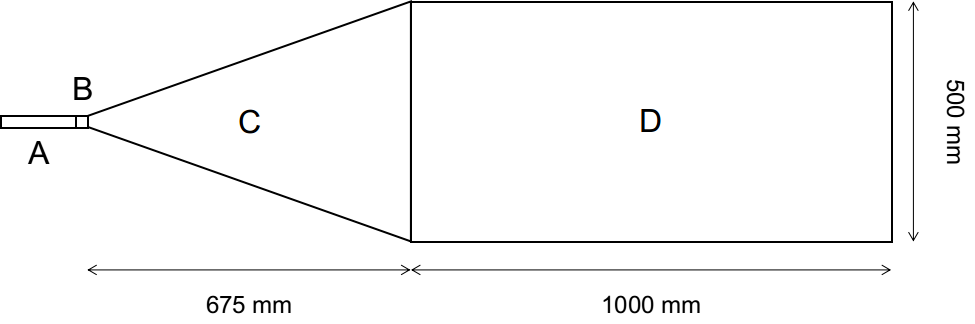
\includegraphics[width=0.75\columnwidth]{config.png}
	\caption{Schematic diagram of the HiSPARC scintillation detector. (A): PMT; (B): light-guide adaptor; (C): light-guide; (D): scintillator.}
	\label{fig:HS_scintillator}
\end{figure}

The scintillator is made of a material consisting of polyvinyltoluene as the base, with anthracene as the fluor, and the emission spectrum peaks at a wavelength of 425~nm \citep{fokkema_hisparc_2012, bartels_hisparc_2012}. The light-guide is made from \gls{pmma} and has a comparable refractive index to the scintillator (1.58 and 1.49, respectively), reducing refraction effects between the two materials \citep{van_dam_hisparc_2020}.

The \gls{pmt} used is an ETEnterprises 9125B \gls{pmt}, with a 25~mm aperture,  blue-green sensitive bialkali photocathode, and 11 high-gain dynodes \citep{bartels_hisparc_2012,et_enterprises_data_2020}. The quantum efficiency of the \gls{pmt} used in the HiSPARC detectors peaks at around 375 nm at 28\%, and at 425 nm the quantum efficiency is 25\% \citep{fokkema_hisparc_2012}. 

Each detector is wrapped in aluminium foil (thickness 30~$\mu$m) and a black, vinyl material (thickness 0.45~mm), which is usually used as a pond liner, to ensure light-tight detectors and to reduce the noise level from stray photons \citep{van_dam_hisparc_2020}. In addition, each detector is placed inside of its own a plastic roof box to again ensure that it is light-tight, and to also ensure that it is weather-proof, as the detectors are usually located on the roofs of schools, colleges, and universities.

A HiSPARC station combines either 2 or 4 detectors, to observe coincident muons (`events'), and typical configurations of each are shown in Figure~\ref{fig:HS_station_layouts}. The separation between detectors varies from station-to-station. In addition some stations have the capability to measure the local atmospheric properties, such as temperature, pressure, relative humidity etc. Moreover, some stations also record the `singles' rates, i.e. the frequency at which an individual detector is triggered, independently of the other detectors in the station. The singles rates are important when investigating non-\gls{eas} events.


\begin{figure}[ht!]
	\centering
	\subfloat[Two-detector station configuration]{
\includegraphics[width=0.6\columnwidth]{HS_2D2.png}} 
	\qquad
	\subfloat[Four-detector station configuration (triangle arrangement)]{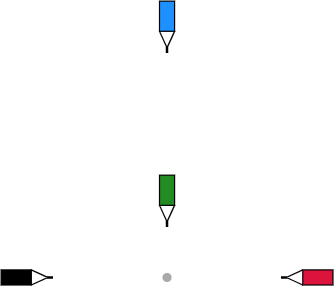
\includegraphics[width=0.6\columnwidth]{HS_4D_t2.png}}
	\qquad
	\subfloat[Four-detector station configuration (diamond arrangement)]{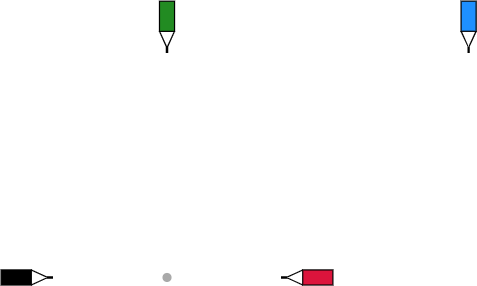
\includegraphics[width=0.6\columnwidth]{HS_4D_d2.png}}
	\caption{Typical formations of two-detector and four-detector stations. In each, the grey circle denotes a GPS antenna which is located in between the detectors to provide a precise timestamp for each signal.}
	\label{fig:HS_station_layouts}
\end{figure}


light pulse which is converted
into an electric pulse by the PMT. This pulse is
sampled and digitized at 400 MHz

The \glspl{pmt} of the detector in a station are connected to HiSPARC electronics boxes, which sample and digitise the signal at a rate of 400~MH, and each \glspl{pmt} is connected to the electronics box using cables of a standard length of 30~m, to minimise any timing offsets between detectors \citep{fokkema_hisparc_2012, van_dam_hisparc_2020}. The electronics boxes are capable of controlling and reading two \glspl{pmt}, therefore a four-detector station requires two electronics boxes: a master and a slave.

The HiSPARC experiment is set up in such a way as to ensure that each station across the HiSPARC network reads a similar count rate of muons, in order to aid the direct comparison between the different stations in the network. When configuring the station, a trigger threshold must be applied for the \gls{pmt} signals. This is standardised across the HiSPARC network and can be seen in relation to a detector trigger pulse in Figure~\ref{fig:HiSPARC_trace}. There are two thresholds, low: 30~mV, which represents 0.2 of a \gls{mip}; high: 70~mV, which represents 0.5 of a \gls{mip} \citep{fokkema_hisparc_2012, van_dam_hisparc_2020}. The thresholds were chosen to increase the sensitivity of the stations for observing gamma rays and low energy electrons, but this has the effect of making it more difficult to determine whether an individual detection is from a muon, or another \gls{mip}. This is why the HiSPARC network usually relies on detecting `events', from coincident muons.

Each detector in the network is set up such that the pulseheight spectrum peaks at a \gls{mpv} of $\sim 150$~mV (see Figure~\ref{fig:pulses}), and such that the high threshold allows a mean count rate on the order 100 counts per second and the low threshold allows a mean count rate of the order 400 counts per second; these can by tuned by adjusting the \gls{pmt} voltage. It could be argued that in setting up the detectors in this way, there is an immediate bias in the data to reject lower energy \glspl{cr}.

\begin{figure}[ht!]
	\centering
	\subfloat[Trigger pulse]{
		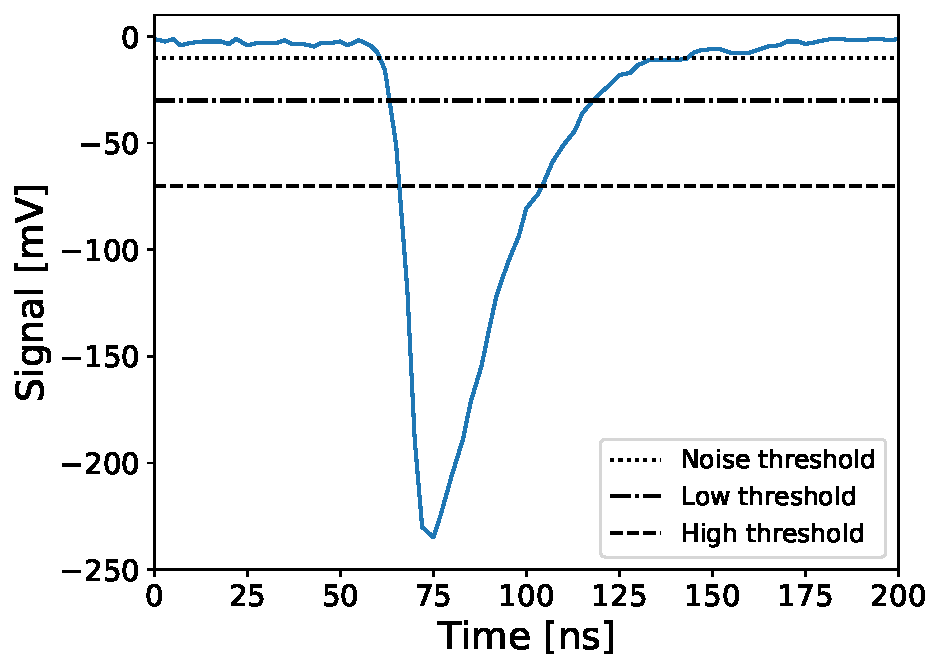
\includegraphics[width=0.48\columnwidth]{trace_plot.pdf}
		\label{fig:HiSPARC_trace}}
	%\qquad
	\subfloat[Pulseheight distribution]{
		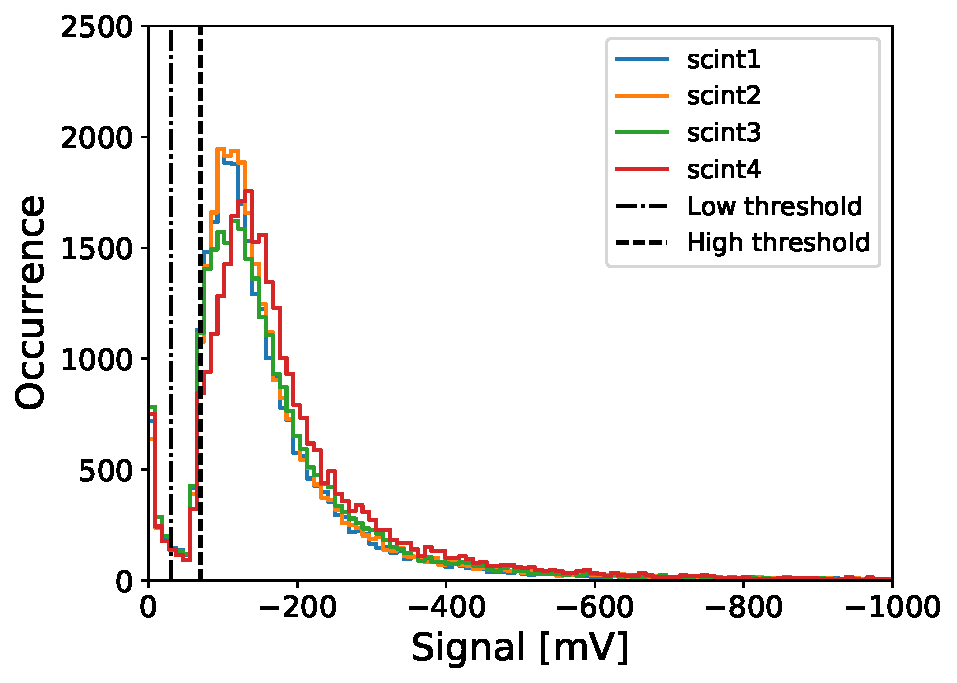
\includegraphics[width=0.48\columnwidth]{pulseheights.pdf}
		\label{fig:HiSPARC_pulseheight}}
	
	\caption{(a): An example PMT signal after digital conversion by the HiSPARC electronics box. The horizontal lines denote: the noise cut-off (dotted line), which is used for setting a limit when integrating the pulse height, to give the pulse integral; the low-voltage threshold (dash-dot); the high-voltage threshold (dashed). (b) The pulse height distribution over the course of a single day from HiSPARC station 501. The vertical lines show the low-voltage threshold (dash-dot) and the high-voltage threshold (dashed).}
	\label{fig:pulses}
\end{figure}

The pulse height spectrum (see Figure~\ref{fig:HiSPARC_pulseheight}) is composed of two main regions: the left side which falls off rather steeply and the main, asymmetric part of the spectrum which features a peak and a long tail. The left side of the spectrum is understood to be from high-energy photons (gamma rays) produced in air showers \citep{fokkema_hisparc_2012}. These high-energy photons may undergo pair production when interacting with the scintillator which may produce ionising electron and positron pairs. The trigger thresholds are placed to reject these noise signals from the data.

The main, asymmetric distribution which features a peak and a tail is from charged particles (muons and electrons) \citep{van_dam_hisparc_2020}. The mean energy loss of particles in a material is described by the Blethe-Bloch formula; however this does not account for fluctuations in energy loss \citep{fokkema_hisparc_2012}. A Landau distribution in fact describes the fluctuations in energy loss of particles. Due to the resolution of the HiSPARC detectors the distribution in Figure~\ref{fig:HiSPARC_pulseheight} is best described by the convolution of the Landau distribution with a normal distribution which describes the resolution of the detector \citep{fokkema_hisparc_2012}. The peak of the distribution, the most probable values (\gls{mpv}), is the most likely energy lost by a particle in the detector, i.e. the 3.51~MeV \gls{mip} \citep{van_dam_hisparc_2020}. It has been shown that the location of the \gls{mpv} can vary due to the effects of atmospheric temperature \citep{bartels_hisparc_2012, van_dam_hisparc_2020}.

The default trigger conditions for detecting an air shower event between multiple \glspl{pmt} within a station differ for a two/four-detector station. In a two-detector station, an event is recorded if the \gls{pmt} signals from both detectors exceed the low threshold within the coincidence time window ($1.5 \, \mu\mathrm{s}$). In a four-detector station, there are two conditions: (i) at least two detectors exceed the high threshold within the coincidence time window; (ii) at least three detectors exceed the low threshold within the coincidence time window. These are the default conditions, but there are other, user configurable ways of triggering the station.

The scientific goals that can be achieved also vary between the two/four-detector stations. When at least three detectors in a four-detector station observe particles of an \gls{eas}, the direction of the \gls{eas} (and thus the direction of the \gls{pcr}) can be acquired using triangulation calculations. When only two detectors in a station observe particles of an \gls{eas}, i.e. the limit for a two-detector station, it is only possible to reconstruct the arrival direction along the axis that connects the centres of those two detectors (thus it is not possible to reconstruct the direction of the \gls{pcr}).




%%%%%%%%%%%%%%%%%%%%%%%%%%%%%%%%%%%%%%%%%%%%%%%%%%%%%%%%%%%%%%%%%%%%%
%%%%%%%%%%%%%%%%%%%%%%%%%%%%%%%%%%%%%%%%%%%%%%%%%%%%%%%%%%%%%%%%%%%%%
\section{Aims}\label{sec:HS_aims}
The HiSPARC project was set up with the detection philosophy of observing \gls{eas}, which are typically associated with \gls{pcr}s with energy of $\sim10^{14}$~eV and above, that produce large footprints observable with many HiSPARC stations simultaneously. For \gls{pcr}s with energy below $\sim10^{14}$~eV the air shower is small, with almost no observable muon footprint, and for \gls{pcr}s with energy below $\sim10^{11}$~eV, there is typically fewer than one or two muons that reach the ground, making their observation difficult. Most muons produced by such low-energy \glspl{pcr} decay higher in the atmosphere and their energy is mostly transferred into the resultant electron \citep{van_dam_hisparc_2020}, which is observable by HiSPARC.

The HiSPARC detectors are capable of observing any muons that reach them, therefore the project was motivated by the existing network of \gls{md} which may have the capability of observing the \gls{cr}s associated with space weather events.

The principle aim of the project was to determine whether the existing HiSPARC network is capable of observing space weather events. To do this, we investigated the properties of the HiSPARC detectors, to learn about what typical \glspl{pcr} we observe. This was initially achieved by investigating the data during periods of space weather activity to search for the associated signatures. We searched through some of the most reliable HiSPARC stations to determine whether these events were observed in the data. This was done to determine whether, without much effort, we could get a binary answer on whether these events were observed by HiSPARC.

Following this, we performed simulations of air showers initiated by \glspl{cr} to understand the expected muon flux and dispersion at ground level. This helped us to understand how likely it is to observe the \glspl{pcr} associated with space weather with the HiSPARC detectors, observing muons.

Finally, ground-based observations of muons from air showers are susceptible to the conditions in the atmosphere; therefore, where possible, we corrected for atmospheric effects and again reviewed the corrected data to determine whether the space weather events were observed.

%%%%%%%%%%%%%%%%%%%%%%%%%%%%%%%%%%%%%%%%%%%%%%%%%%%%%%%%%%%%%%%%%%%%%
%%%%%%%%%%%%%%%%%%%%%%%%%%%%%%%%%%%%%%%%%%%%%%%%%%%%%%%%%%%%%%%%%%%%%
\section{HiSPARC Properties}\label{sec:HS_properties}

To understand the \gls{pcr} spectrum that the HiSPARC stations are capable of observing, \gls{pcr} transport simulations were performed using the PLANETOCOSMICS software. PLANETOCOSMICS performs Geant4 Monte Carlo simulations of charged particle transport through Earth's magnetosphere based on St\o rmers transport equation for charged particles \citep{desorgher_planetocosmics_2006}. PLANETOCOSMICS simulates backward trajectories of charged particles from a given location (latitude, longitude, and altitude) out to the magnetopause for a set of \gls{pcr} rigidities. 

For each trajectory there are two possible outcomes: (i) the particles trace out to the magnetopause where they escape Earth's magnetosphere, an allowed trajectory; (ii) the particles are sufficiently bent by the effect of the Earth's magnetosphere that they do not reach the magnetopause and cannot escape the Earth's magnetosphere, a forbidden trajectory \citep{desorgher_planetocosmics_2006}. The coordinates of the asymptotic direction at the magnetosphere are provided as an output to the simulations projected back down to the Earth's surface. In this work PLANETOCOSMICS was configured with the Tsyganenko-89 model for the external magnetospheric magnetic field and the \gls{igrf} internal field model.

For each rigidity simulated, whether it was an allowed or forbidden trajectory was stored, which was used to provide an insight into the rigidity spectrum for a given station. From the allowed trajectories the effective cut-off rigidity ($R_C$) for the stations was computed using equation~(\ref{eq:cut_off}), where $R_U$ is the upper rigidity (the last allowed trajectory before the first forbidden trajectory); $R_L$ is the lower rigidity (the last allowed trajectory before which all other trajectories with a lower rigidity are forbidden); $\Delta R$ is the rigidity step size in the simulation \citep{desorgher_planetocosmics_2006, herbst_influence_2013}.

\begin{equation}
\label{eq:cut_off}
R_C = R_U - \sum_{i = R_L}^{R_U} \Delta R_i
\end{equation}

The rigidity spectrum for each of the HiSPARC stations were investigated to determine $R_C$ for each station. The cut-off rigidity calculated for the six HiSPARC stations for a vertical incidence upon the atmosphere (i.e. $0^\circ$ zenith angle) are shown in Table~\ref{tab:HS_stns} which show that there is little variation in $R_C$ between the HiSPARC stations and that they observe protons with rigidities in excess of $\sim 3$~GV. This analysis was initially carried out for the vertical direction (i.e. azimuth = $0^\circ$, zenith = $0^\circ$); however further trajectories were simulated for different azimuth and zenith angles to determine the dependence of the rigidity spectrum on the detector acceptance angle. The analysis for the azimuthal dependence was carried out at a zenith angle of $20^\circ$ as this is around the most probably angle for HiSPARC events, and the analysis of the zenith dependence was carried out at an azimuth angle of $0^\circ$.


\begin{table}
	\begin{center}
		\caption{Properties of some of the HiSPARC stations: geographic longitude ($\lambda$), geographic latitude ($\phi$), altitude ($h$), and the geomagnetic vertical cut-off rigidity ($R_C$) calculated from the PLANETOCOSMICS simulations.}
		\label{tab:HS_stns}
		\begin{tabular}{l c c c c c}
			\hline
			& $R_C$  & $\lambda$ & $\phi$  & $h$  & No. Detectors\\
			Station Name/ID & [GV] & [deg] & [deg] & [m]  & \\
			\hline
			Nikhef/501 & 3.19 & 4.95 E & 52.36 N & 56.18 & 4 \\
			College Hageveld/203 & 3.18 & 4.63 E  & 52.35 N & 53.71  & 2 \\
			Leiden/3001 & 3.23 & 4.45 E & 52.17 N & 54.08 & 2 \\
			Eindhoven/8001  & 3.44 & 5.49 E & 51.45 N & 70.12 & 2 \\
			Birmingham University/14001  & 3.06 & 1.93 W & 52.45 N & 204.14 & 4  \\
			%20003 & 2.30 & 10.20 E & 56.17 N & 84.38 & 2 \\
			\hline
		\end{tabular}
	\end{center}
\end{table}

\begin{figure}[h]
	\centering
	\subfloat[Azimuth variation (fixed zenith = $20^\circ$)]{
		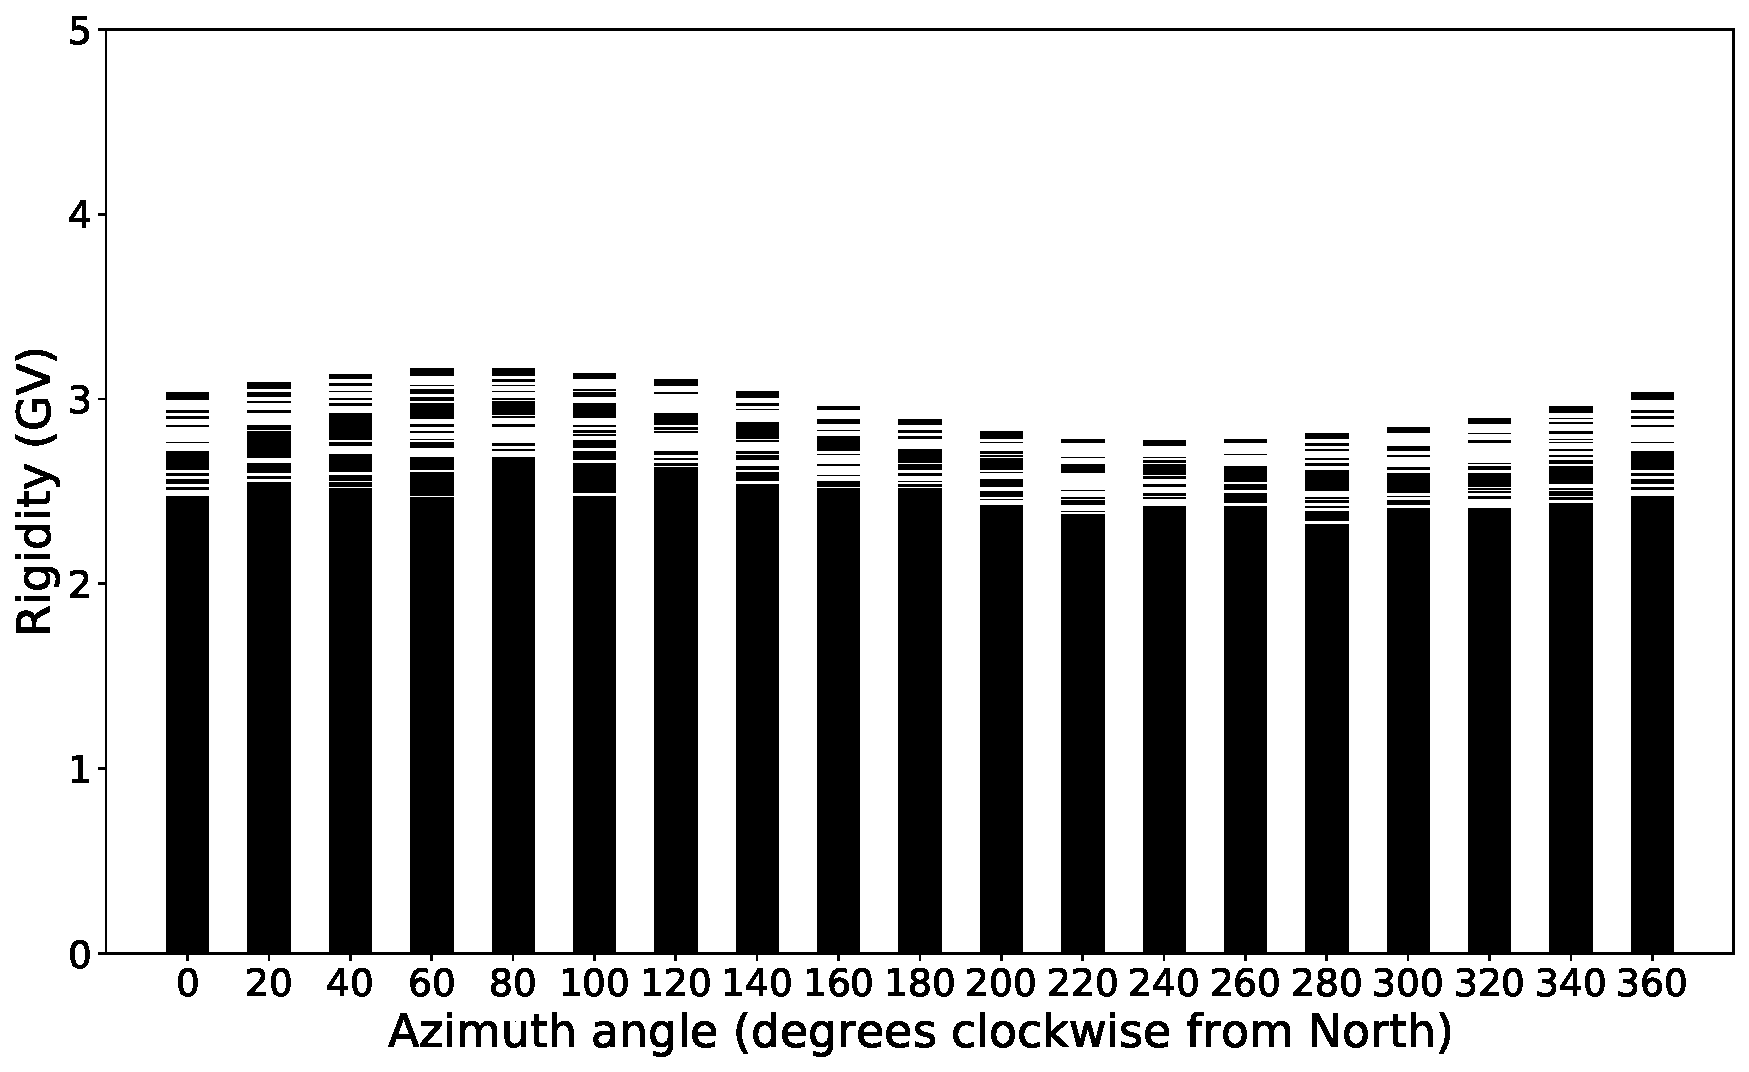
\includegraphics[width=0.48\columnwidth]{azm.pdf}
		\label{fig:azm1}}
	%\qquad
	\subfloat[Zenith variation (fixed azimuth = $0^\circ$)]{
		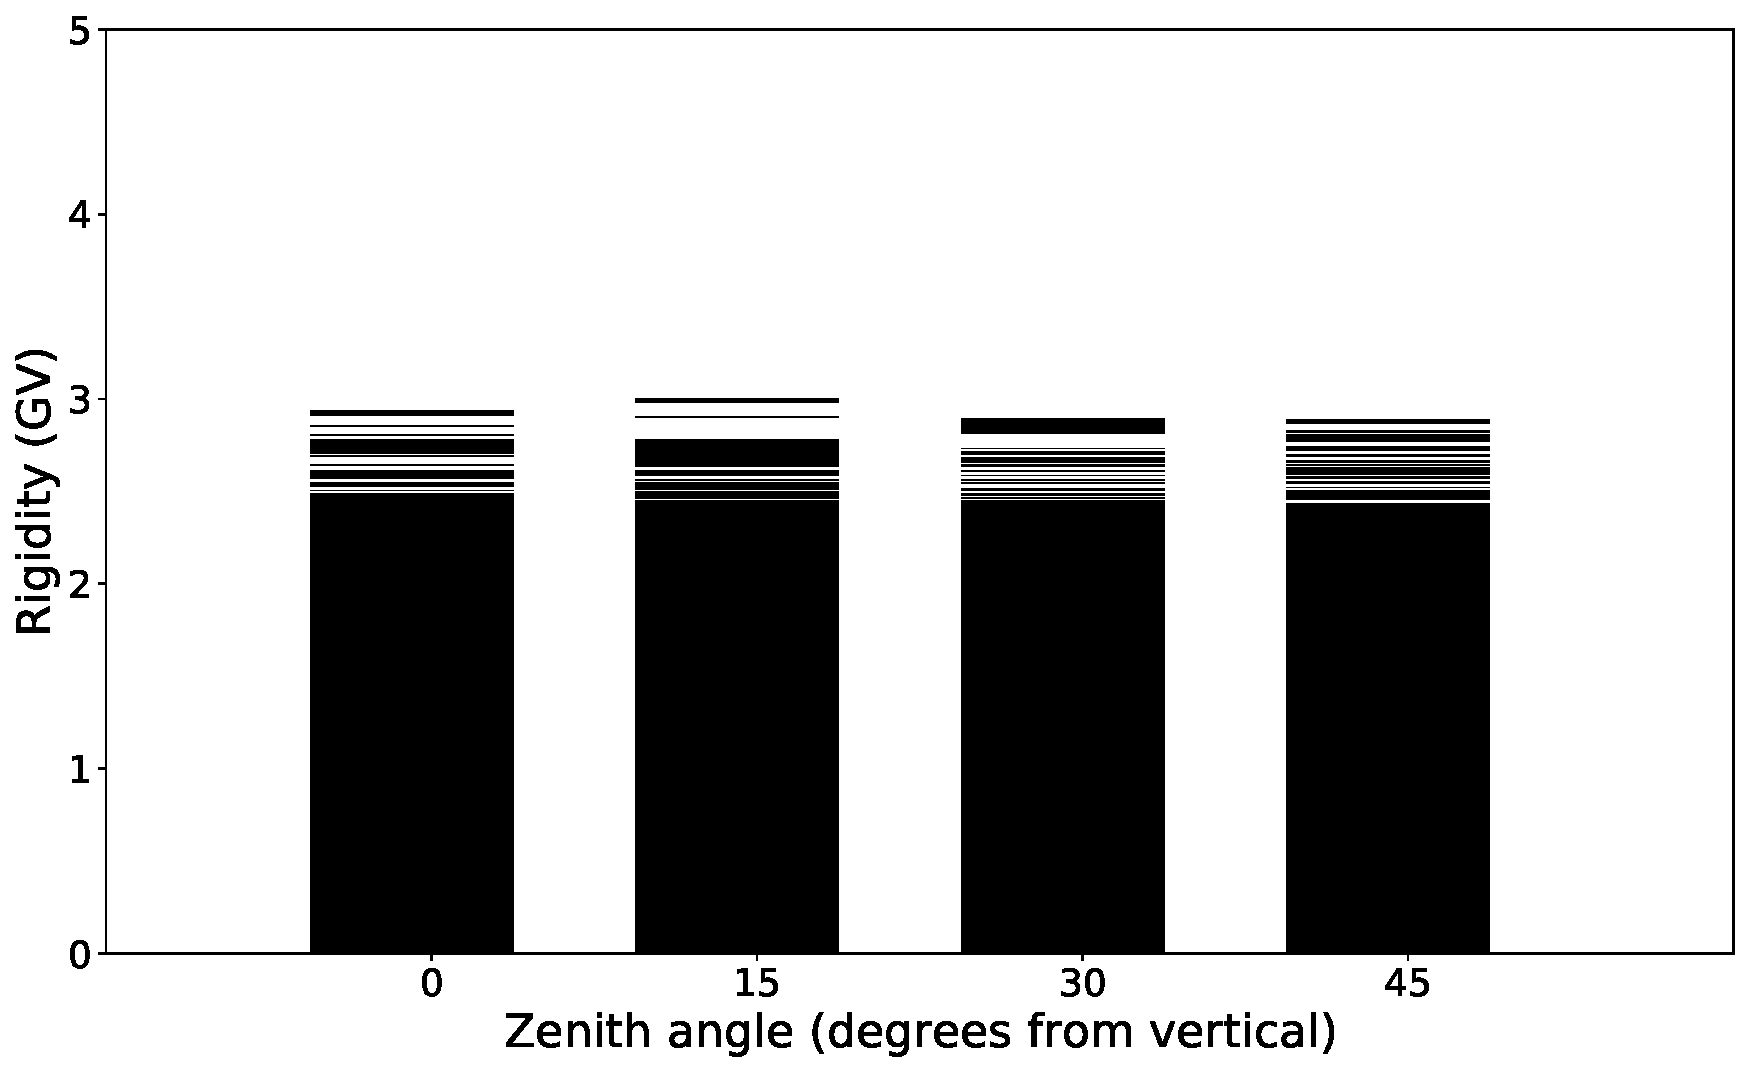
\includegraphics[width=0.48\columnwidth]{zen.pdf}
		\label{fig:zen1}}
	
	\caption{Azimuthal and zenith angle variations in the allowed and forbidden rigidity trajectories for HiSPARC station 501.}
	\label{fig:R_C2}
\end{figure}

The small variation between HiSPARC stations is due to their close proximity in geographic latitude and longitude. The values of $R_C$ calculated for the HiSPARC stations suggest that they should be able to observe higher energy \gls{scr}, but may not be as susceptible as the higher latitude \gls{nm} where the effects of \glspl{gle} are highly observable.

As a results of the PLANETOCOSMICS simulations it was possible to understand the trajectories of particles that enter the Earth's magnetosphere prior to arrival at the atmosphere. It can be seen from Figure~\ref{fig:HS_AVD} that the \glspl{avd} for each of the HiSPARC stations investigated are rather similar, and that they mostly straddle the equator for low rigidity \glspl{pcr}. 

\begin{figure}[ht!]
	\centering
	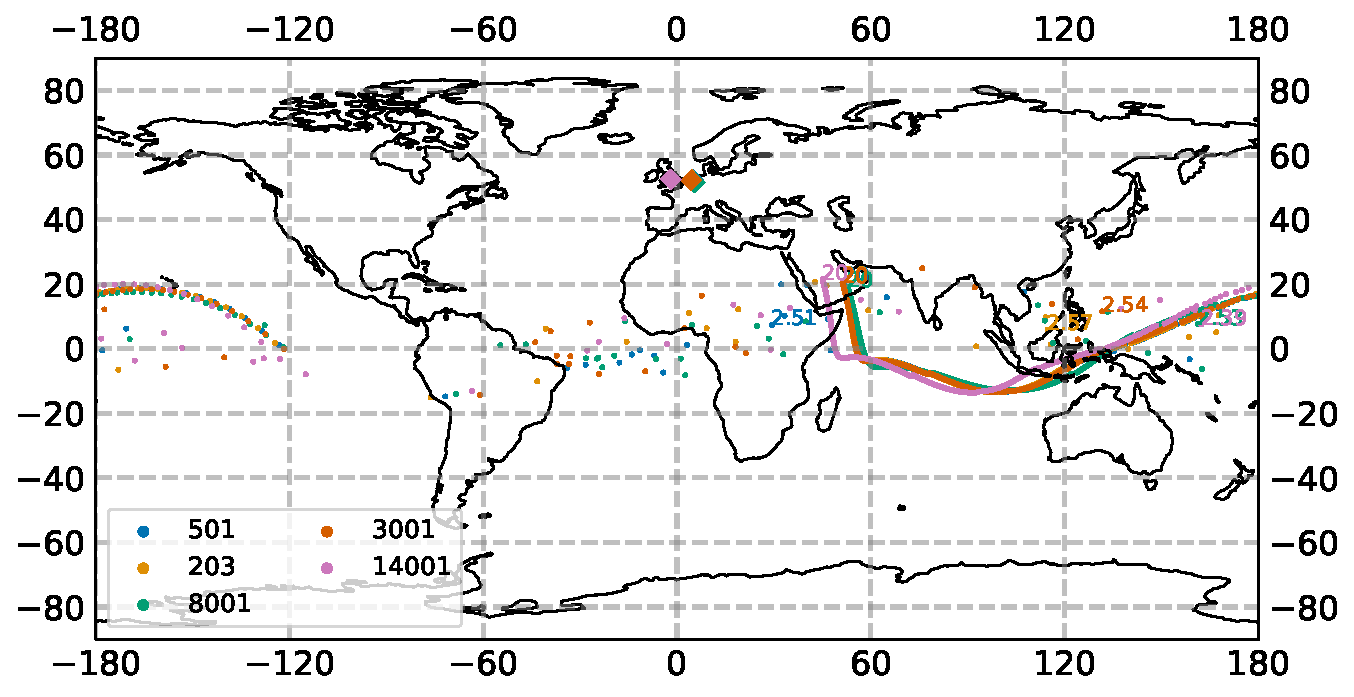
\includegraphics[scale=0.6]{HS_AVDs.pdf}
	\caption{The vertical asymptotic viewing directions of 5 HiSPARC stations. The rigidity range of the simulations were from $1.0$~GV $<$ R $<20.0$~GV, and the results are plotted in geographic coordinates on January 20th 2005. The diamonds correspond to the HS ground location and the circles correspond to the AVD for a specific rigidity value.}
	\label{fig:HS_AVD}
\end{figure}

The simulations were only performed up to a rigidity of 20~GV; however, at higher rigidities, we would see the \glspl{avd} spiral in towards the geographic location of the station, and the \gls{pcr} would enter the magnetosphere and atmosphere almost vertically above the detector. This map of the \glspl{avd} also informs us that we should expect to be able to observe some lower energy \glspl{pcr} when the zenith of the detector is not facing the asymptotic direction of the \gls{pcr}.

%%%%%%%%%%%%%%%%%%%%%%%%%%%%%%%%%%%%%%%%%%%%%%%%%%%%%%%%%%%%%%%%%%%%%
%%%%%%%%%%%%%%%%%%%%%%%%%%%%%%%%%%%%%%%%%%%%%%%%%%%%%%%%%%%%%%%%%%%%%
\section{HiSPARC Observations}\label{sec:HS_obs}


[...!!...end with discussion on unknown \glspl{pcr} observable and the effect of atmospheric weather conditions that need to be accounted for...]

The effects of space weather on \glspl{cr} has been outlined in [REF intro]. It was highlighted during private communication with the UK Met Office that observations of \glspl{gle} are of more interest and importance to space weather forecasts and nowcasts. \glspl{fd} are of lower interest and importance, we still searched for \glspl{fd} within the HiSPARC data. Table~\ref{tab:space_weather_events} outlines the specific space weather driven \glspl{gle} and \glspl{fd} that we searched for within the HiSPARC data.

%\begin{table}
%	\begin{center}
%		\caption{Space weather events investigated within the HiSPARC data. The percentage change column provides a reference of how much the CR counts observed by the NM station at Oulu (R$_c$=0.81~GV) increased of decreased by, due to the space weather event. More precise times for the event onset can be found at \citet{nmdb_nmdb_nodate} (for GLEs) and \citet{lingri_forbush_2016} (for FDs).}
%		\label{tab:space_weather_events}
%		\begin{tabular}{c c c | c c}
%		\hline
%		{\bf GLE Onset} & {\bf GLE} & {\bf \% Change (Oulu)} & {\bf FD Onset} & {\bf \% Change (Oulu)}\\
%		\hline
%		{13/12/2006} & {70} & {$\sim 90\%$} & {08/03/2012} & {$\sim 10\%$}  \\
%		{17/05/2012} & {71} & {$\sim 15\%$} & {12/03/2012} & {$\sim 3-5\%$} \\
%		{10/09/2017} & {72} & {$\sim 5\%$} & {14/07/2012} & {$\sim 3\%$} \\
%		{} & {} & {} & {21/12/2014} & {$\sim 5\%$} \\
%		{} & {} & {} & {06/09/2017} & {$\sim 2\%$} \\
%		{} & {} & {} & {07/09/2017} & {$\sim 8\%$} \\
%		\hline
%		\end{tabular}
%	\end{center}
%\end{table}

\begin{table}
	\begin{center}
		\caption{Space weather events investigated within the HiSPARC data. The percentage change column provides a reference of how much the CR counts observed by the NM station at Oulu (R$_c$=0.81~GV) and Irktutsk (R$_c$=3.64~GV) increased of decreased by, due to the space weather event. More precise times for the event onset can be found at \citet{nmdb_nmdb_nodate} (for GLEs) and \citet{lingri_forbush_2016} (for FDs).}
		\label{tab:space_weather_events}
		\begin{tabular}{c c c c | c c c}
			\hline
			{\bf GLE Onset} & {\bf GLE} & \multicolumn{2}{c |}{\bf \% Change} & {\bf FD Onset} & \multicolumn{2}{c}{\bf \% Change}\\
			{} & {} & {\bf Oulu} & {\bf Irktutsk} & {} & {\bf Oulu} & {\bf Irktutsk}\\			
			
			\hline
			{13/12/2006} & {70} & {$\sim 90\%$} & {$\sim 5\%$} & {08/03/2012} & {$\sim 10\%$}  & {$\sim 10\%$} \\
			{17/05/2012} & {71} & {$\sim 15\%$} & {$\sim 1\%$} & {12/03/2012} & {$\sim 3-5\%$} & {$\sim 3-5\%$} \\
			{10/09/2017} & {72} & {$\sim 5\%$} & {$\sim 2\%$} & {14/07/2012} & {$\sim 3-5\%$} & {$\sim 3-5\%$} \\
			{} & {} & {} & {} & {21/12/2014} & {$\sim 5-10\%$} & {$\sim 5-10\%$} \\
			{} & {} & {} & {} & {06/09/2017} & {$\sim 1-2\%$} & {$\sim 1-2\%$} \\
			{} & {} & {} & {} & {07/09/2017} & {$\sim 6\%$} & {$\sim 7\%$} \\
			\hline
		\end{tabular}
	\end{center}
\end{table}

The specific events in Table~\ref{tab:space_weather_events} were selected as: (i) for the \glspl{gle}, they are the only three that fall in the HiSPARC operational period; (ii) for the \glspl{fd}, they are the only individual, or set of, \glspl{fd} that result in a count variation in excess of $\sim 5\%$ and the largest \glspl{fd} are likely to be the most promising candidates for observation with HiSPARC.

For comparison with the HiSPARC results shown below, we show the \glspl{gle}, as observed by the Oulu \gls{nm} station, in Figure~\ref{fig:oulu_gles}. It is clear from Figure~\ref{fig:oulu_gles} that the relative increase of the \glspl{gle} was large for \gls{gle} 70 and 71, but much more subtle for \glspl{gle} 72. We expect that if we are to observe any of the GLEs, we shall have the best chance of observing \glspl{gle} 70. 

\begin{figure}[ht!]
	\centering
	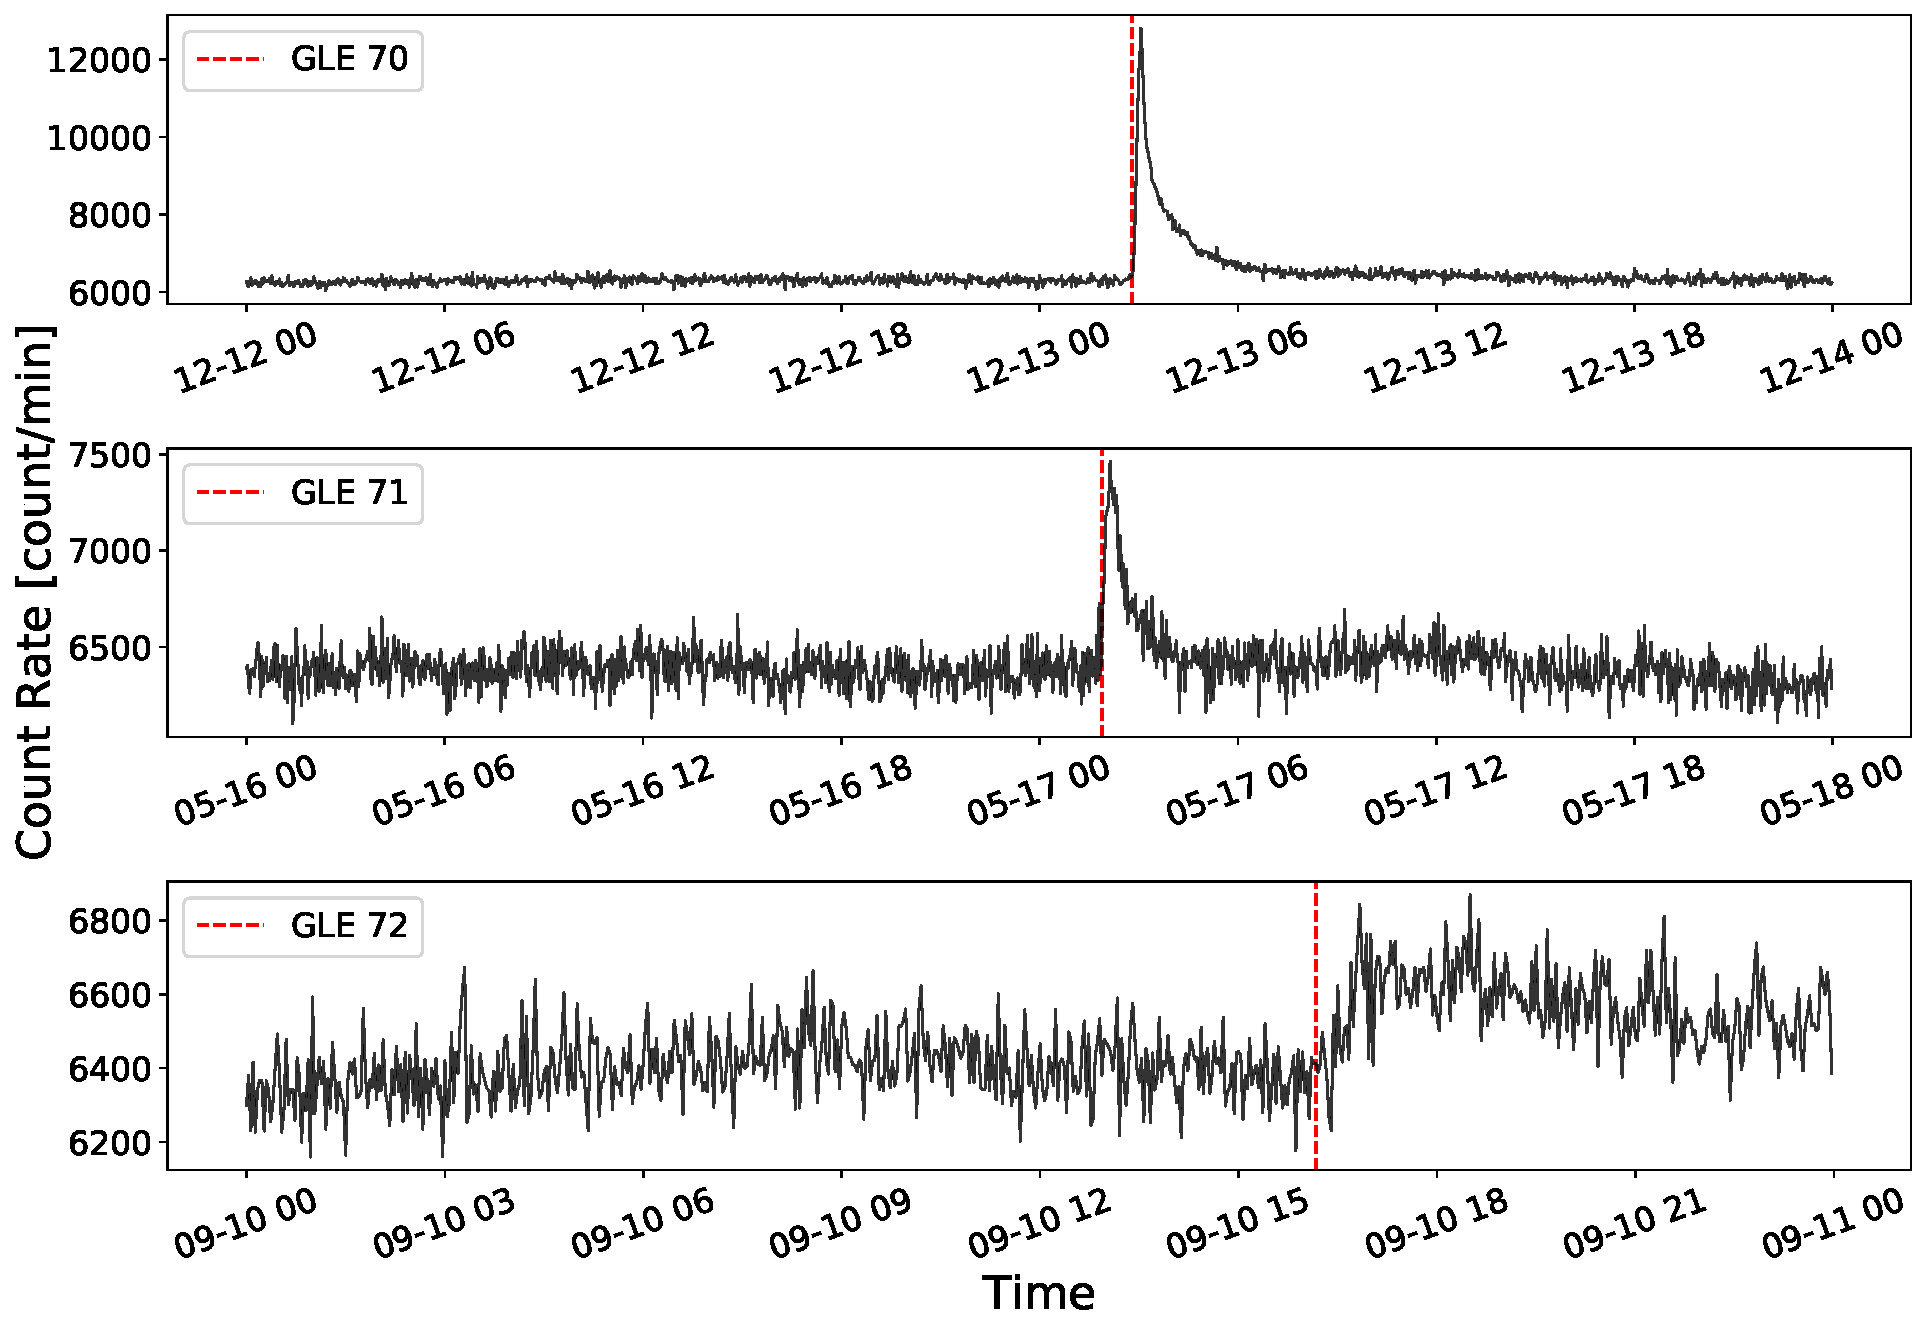
\includegraphics[width=0.75\columnwidth]{GLEs_OULU.pdf}
	\caption{GLEs observed by the NM stations based at Oulu. Top panel: GLE 70; middle panel: GLE 71, bottom panel: GLE 72. The solid-black line shows the 2-minute-averaged, pressure corrected data and the vertical, dashed-red lines show the epochs of each GLE onset. The units of time on the x-axis are, MM-DD HH.}
	\label{fig:oulu_gles}
\end{figure}

Similarly, we show a comparison plot for the \glspl{fd}, as observed by the Oulu \gls{nm} station, in Figure~\ref{fig:oulu_fds}.

\begin{figure}[ht!]
	\centering
	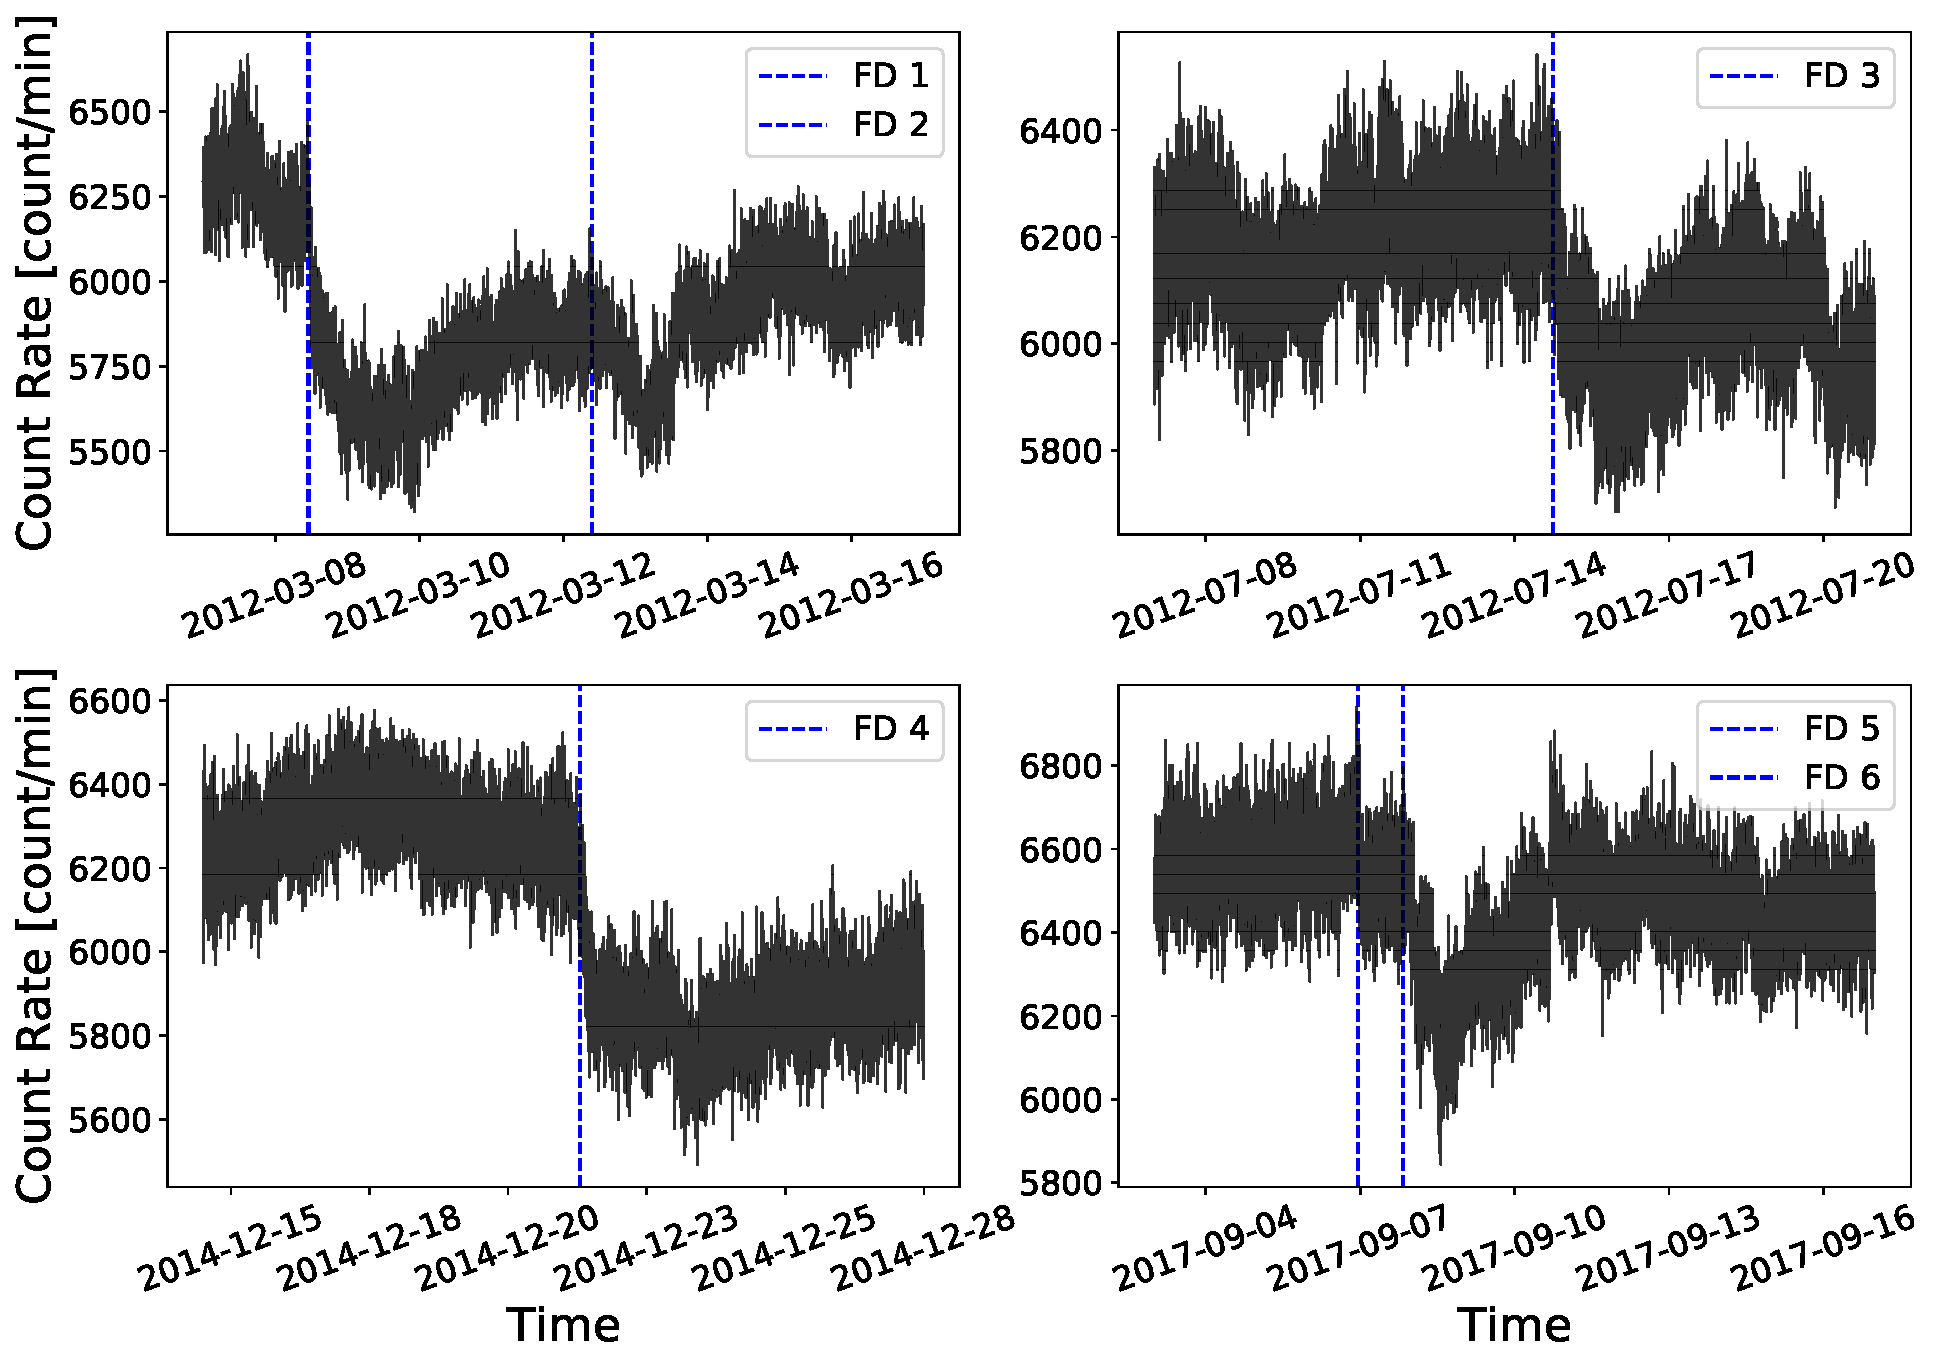
\includegraphics[width=0.75\columnwidth]{FDs_OULU.pdf}
	\caption{FDs observed by the NM stations based at Oulu. Top left panel: FDs during March 2012; top right panel: FD during July 2012, bottom left panel: FD during December 2014; bottom right panel: FD during September 2017. The solid-black line shows the 2-minute-averaged, pressure corrected data and the vertical, dashed-blue lines show the epochs of each FD onset. The units of time on the x-axis are, YYYY-MM-DD.}
	\label{fig:oulu_fds}
\end{figure}

As there are only a few space weather events that we were particularly interested in, and only a few HiSPARC stations that we felt were reliable for our investigation, we conducted the search for these \glspl{gle} and \glspl{fd} by-eye in the data
.

%%%%%%%%%%%%%%%%%%%%%%%%%%%%%%%%%%%%%%%%%%%%%%%%%%%%%%%%%%%%%%%%%%%%%
\subsection{HiSPARC Observations of Ground Level Enhancements}

The search for evidence of \glspl{gle} within the HiSPARC data was conducted for \gls{gle} 70, 71, and 72, as they are the only \glspl{gle} that span the operational epoch of the HiSPARC network. Figure~\ref{fig:GLE_70}, Figure~\ref{fig:GLE_71}, and Figure~\ref{fig:GLE_72} shows the HiSPARC observations around the epochs of \gls{gle} 70, 71, and 72, respectively.

Most of the observations show only the HiSPARC events data (i.e. coincidences between the detectors of a station); however, where possible, we also show the singles rates from each of the individual detectors in a station when the singles rate data is available.

\begin{figure}[ht!]
	\centering
	\subfloat[HS 501 (Nikhef)]{
		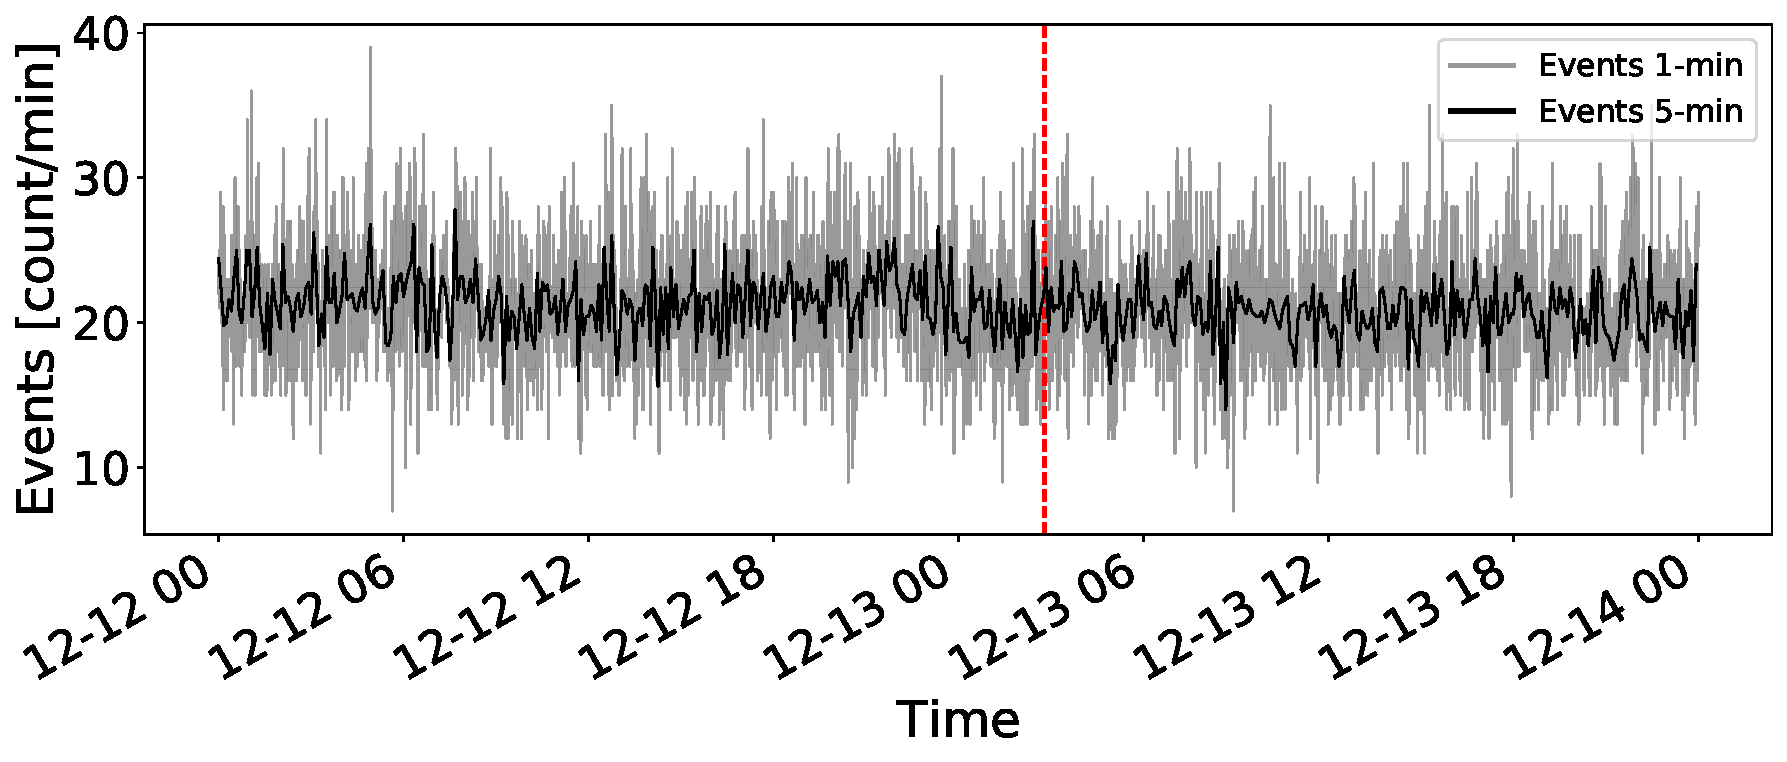
\includegraphics[width=0.48\columnwidth]{GLE70_501.pdf}
		\label{fig:GLE70_501}}
	%\qquad
	\subfloat[HS 3001 (Universiteit Leiden)]{
		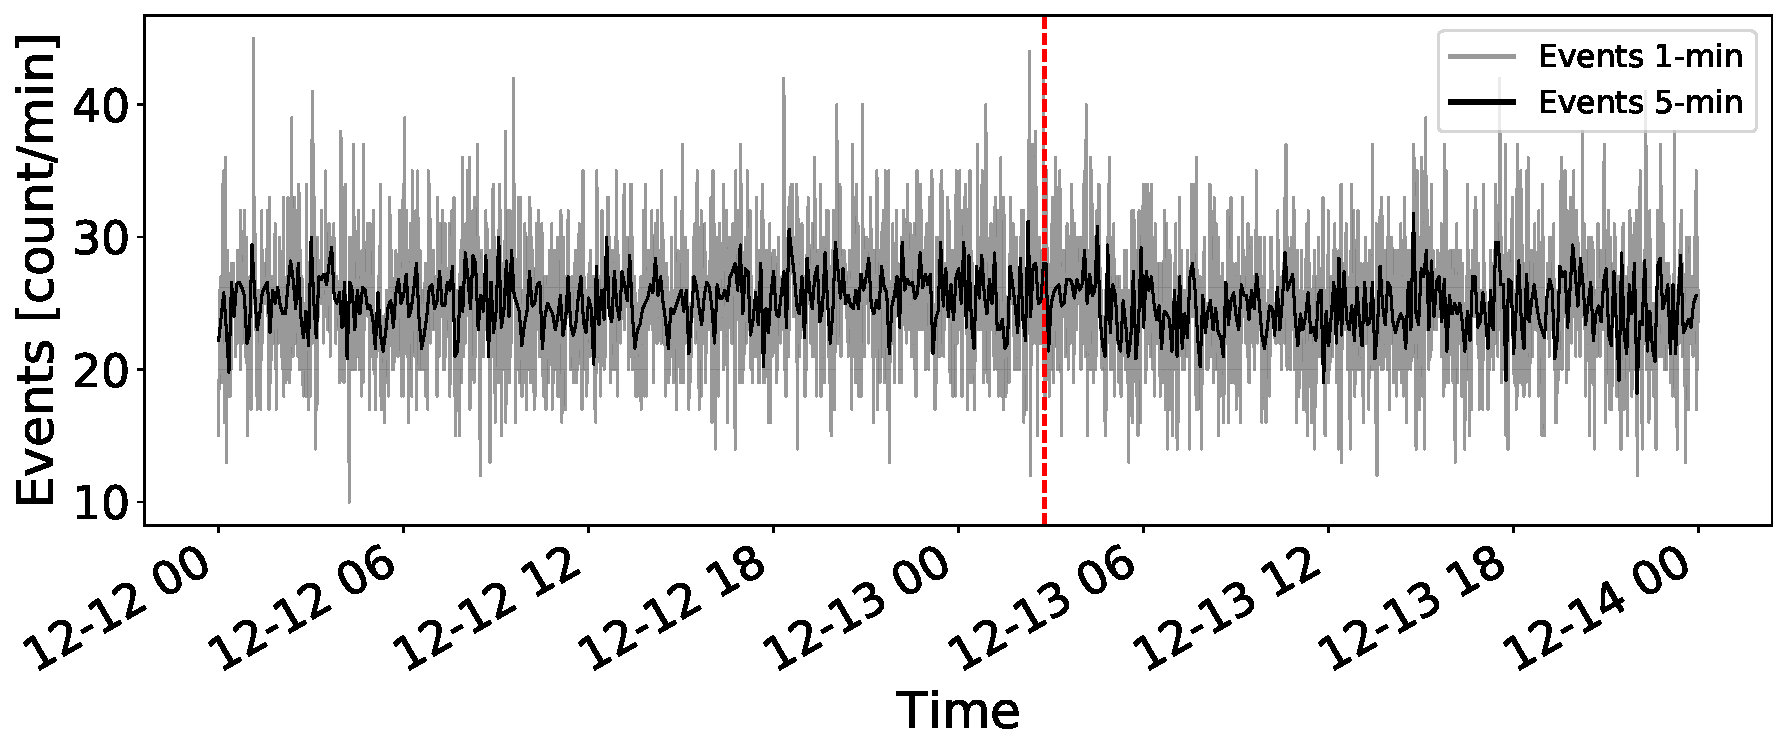
\includegraphics[width=0.48\columnwidth]{GLE70_3001.pdf}
		\label{fig:GLE70_3001}}
	
	\caption{HiSPARC data for stations 501 and 3001 around the epoch of GLE 70. The plot shows the minute-averaged and 5-minute-averaged trigger events between detectors within the station. The vertical red, dashed line depicts the approximate onset time of the GLE. The units of time on the x-axis are, MM-DD HH.}
	\label{fig:GLE_70}
\end{figure}

\begin{figure}[ht!]
	\centering
	\subfloat[HS 8001 (Eindhoven)]{
		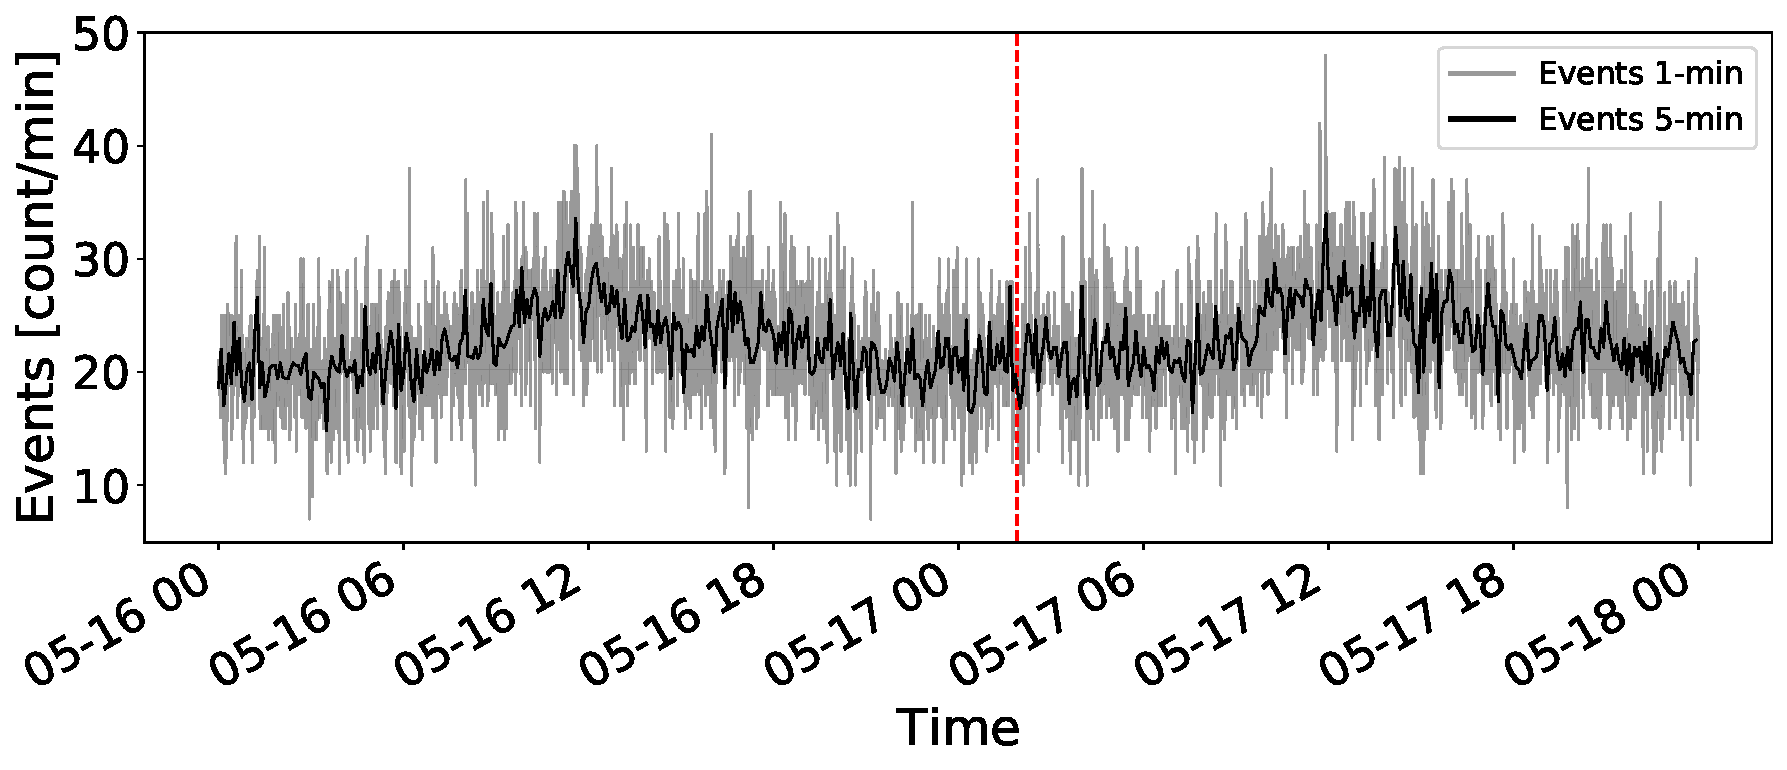
\includegraphics[width=0.48\columnwidth]{GLE71_8001.pdf}
		\label{fig:GLE71_8001}}
	%\qquad
	\subfloat[HS 3001 (Universiteit Leiden)]{
		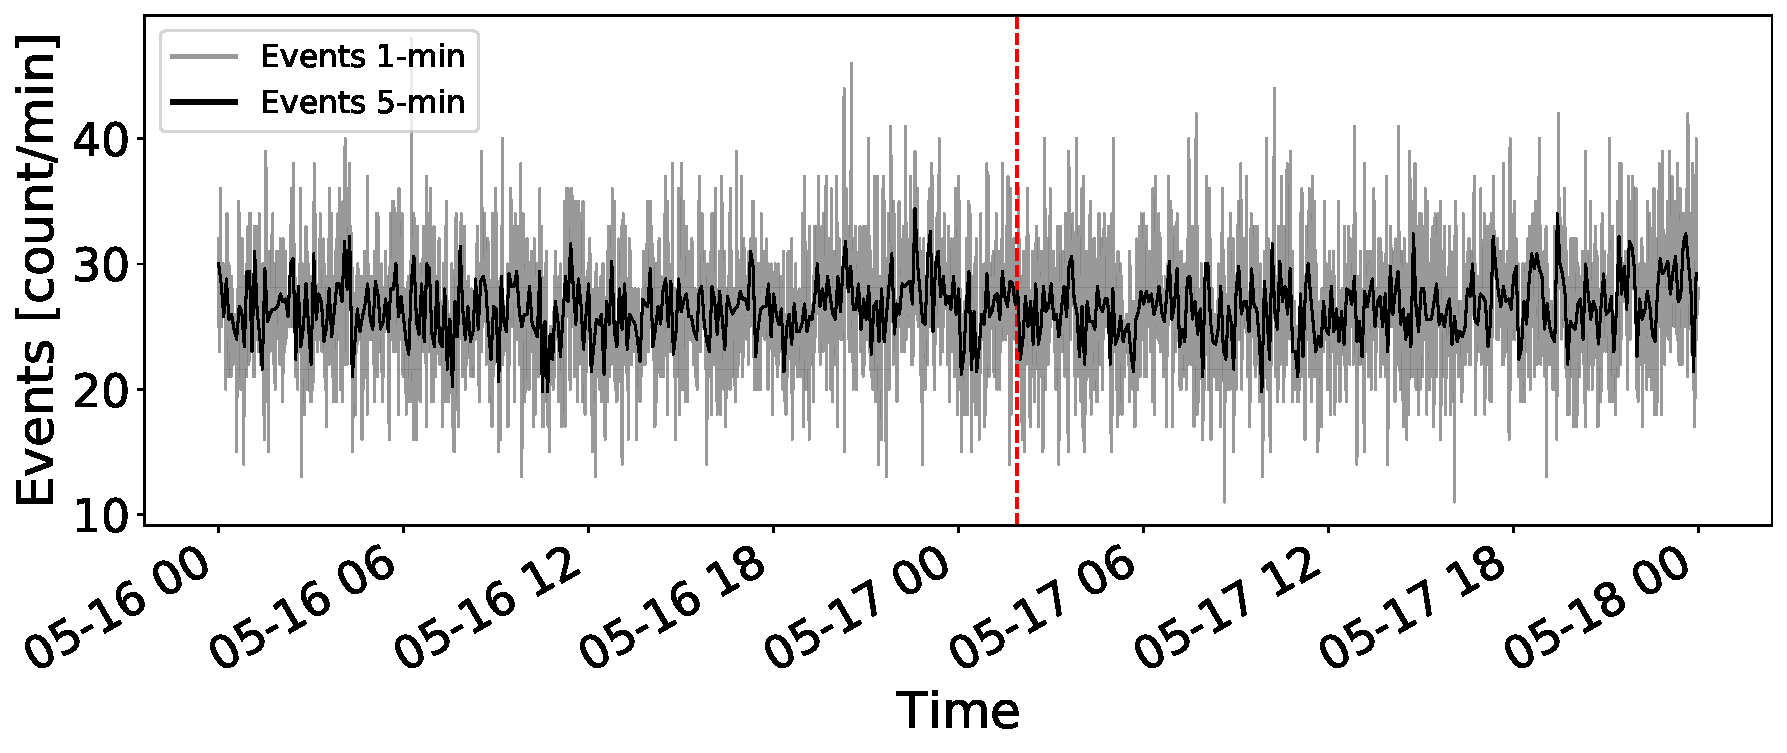
\includegraphics[width=0.48\columnwidth]{GLE71_3001.pdf}
		\label{fig:GLE71_3001}}
	
	\caption{HiSPARC data for stations 8001 and 3001 around the epoch of GLE 71. The plot shows the minute-averaged and 5-minute-averaged trigger events between detectors within the station. The vertical red, dashed line depicts the approximate onset time of the GLE. The units of time on the x-axis are, MM-DD HH.}
	\label{fig:GLE_71}
\end{figure}

\begin{figure}[ht!]
	\centering
	\subfloat[HS 501 (Nikhef)]{
		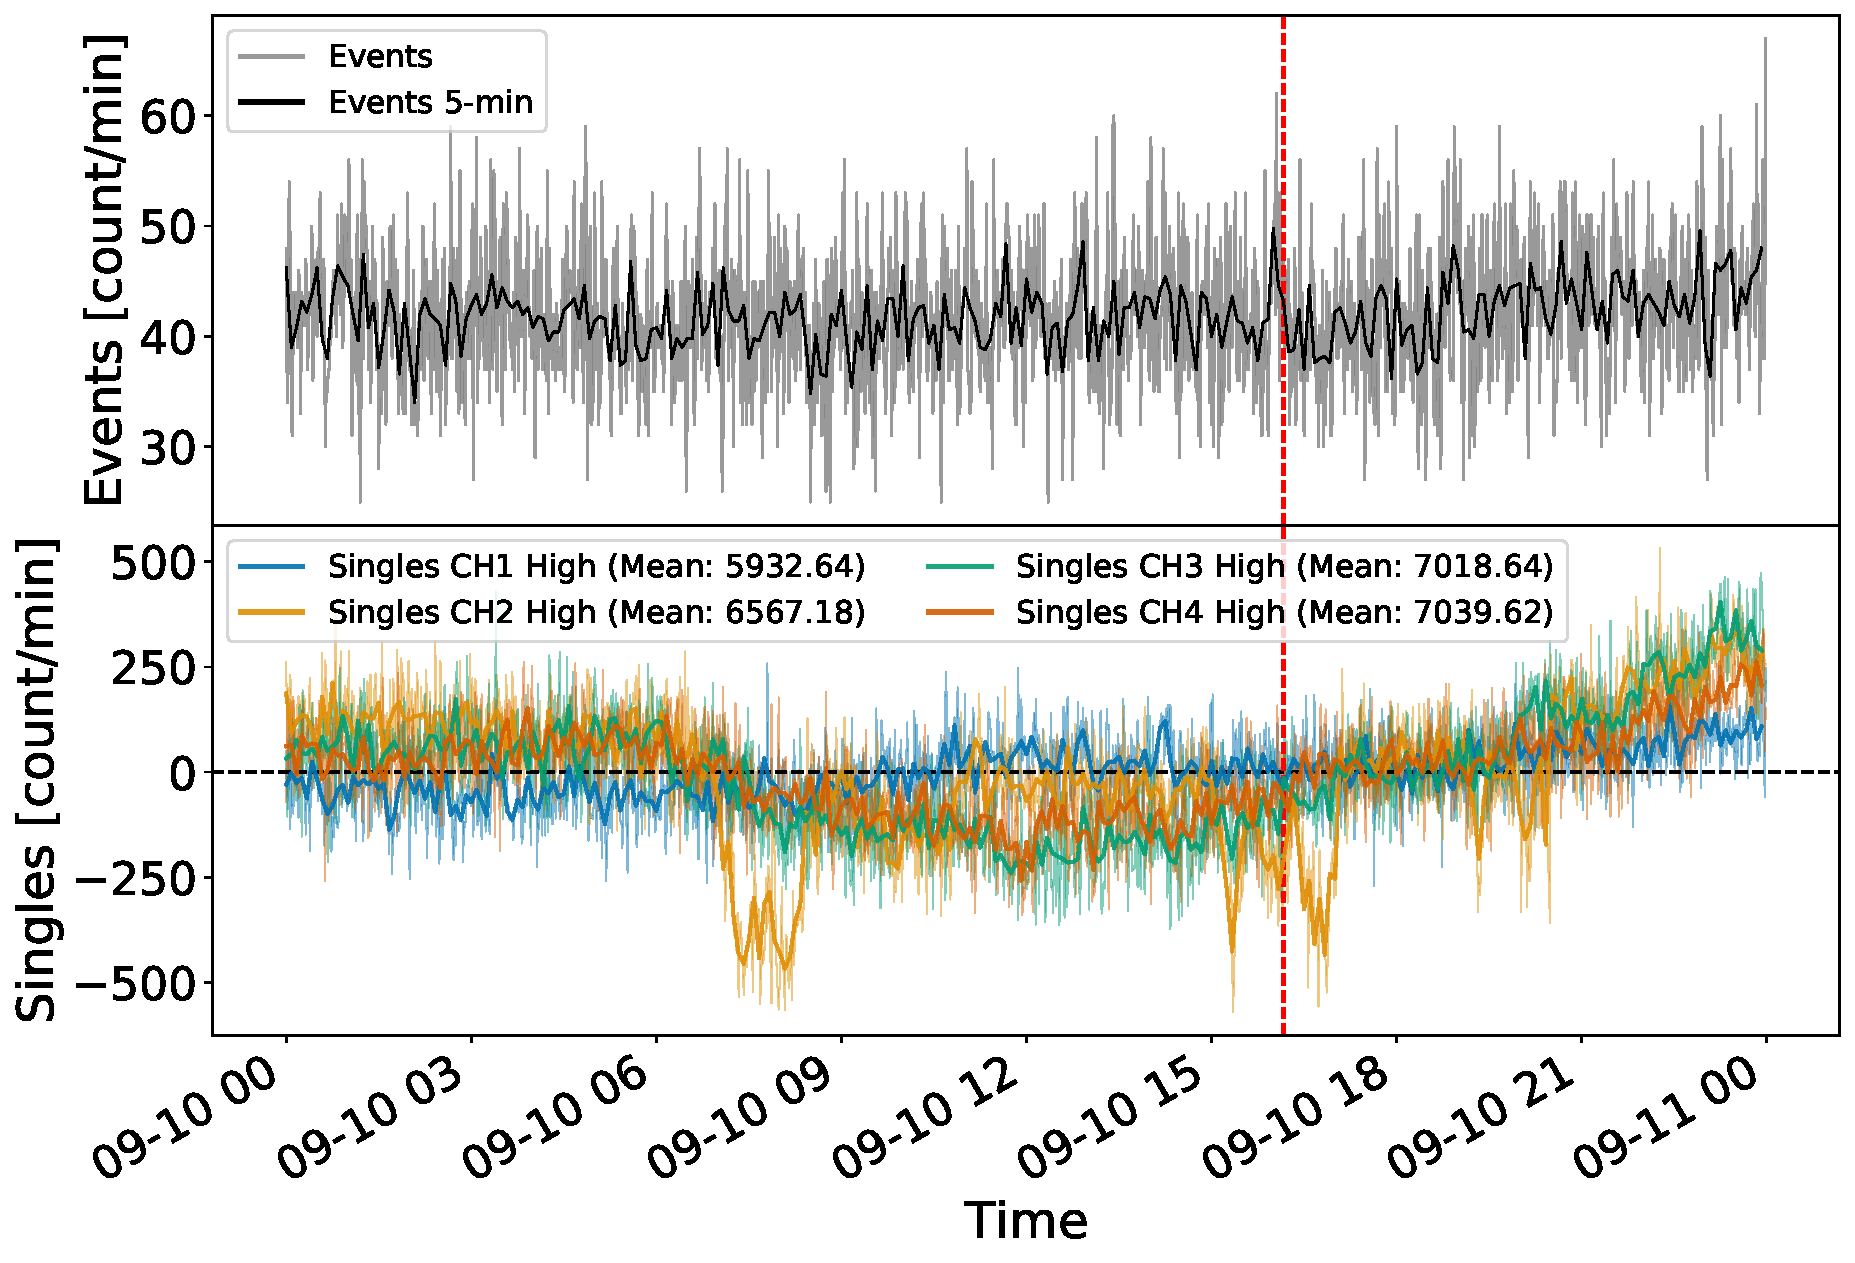
\includegraphics[width=0.48\columnwidth]{GLE72_501.pdf}
		\label{fig:GLE72_501}}
	%\qquad
	\subfloat[HS 203 (College Hageveld)]{
		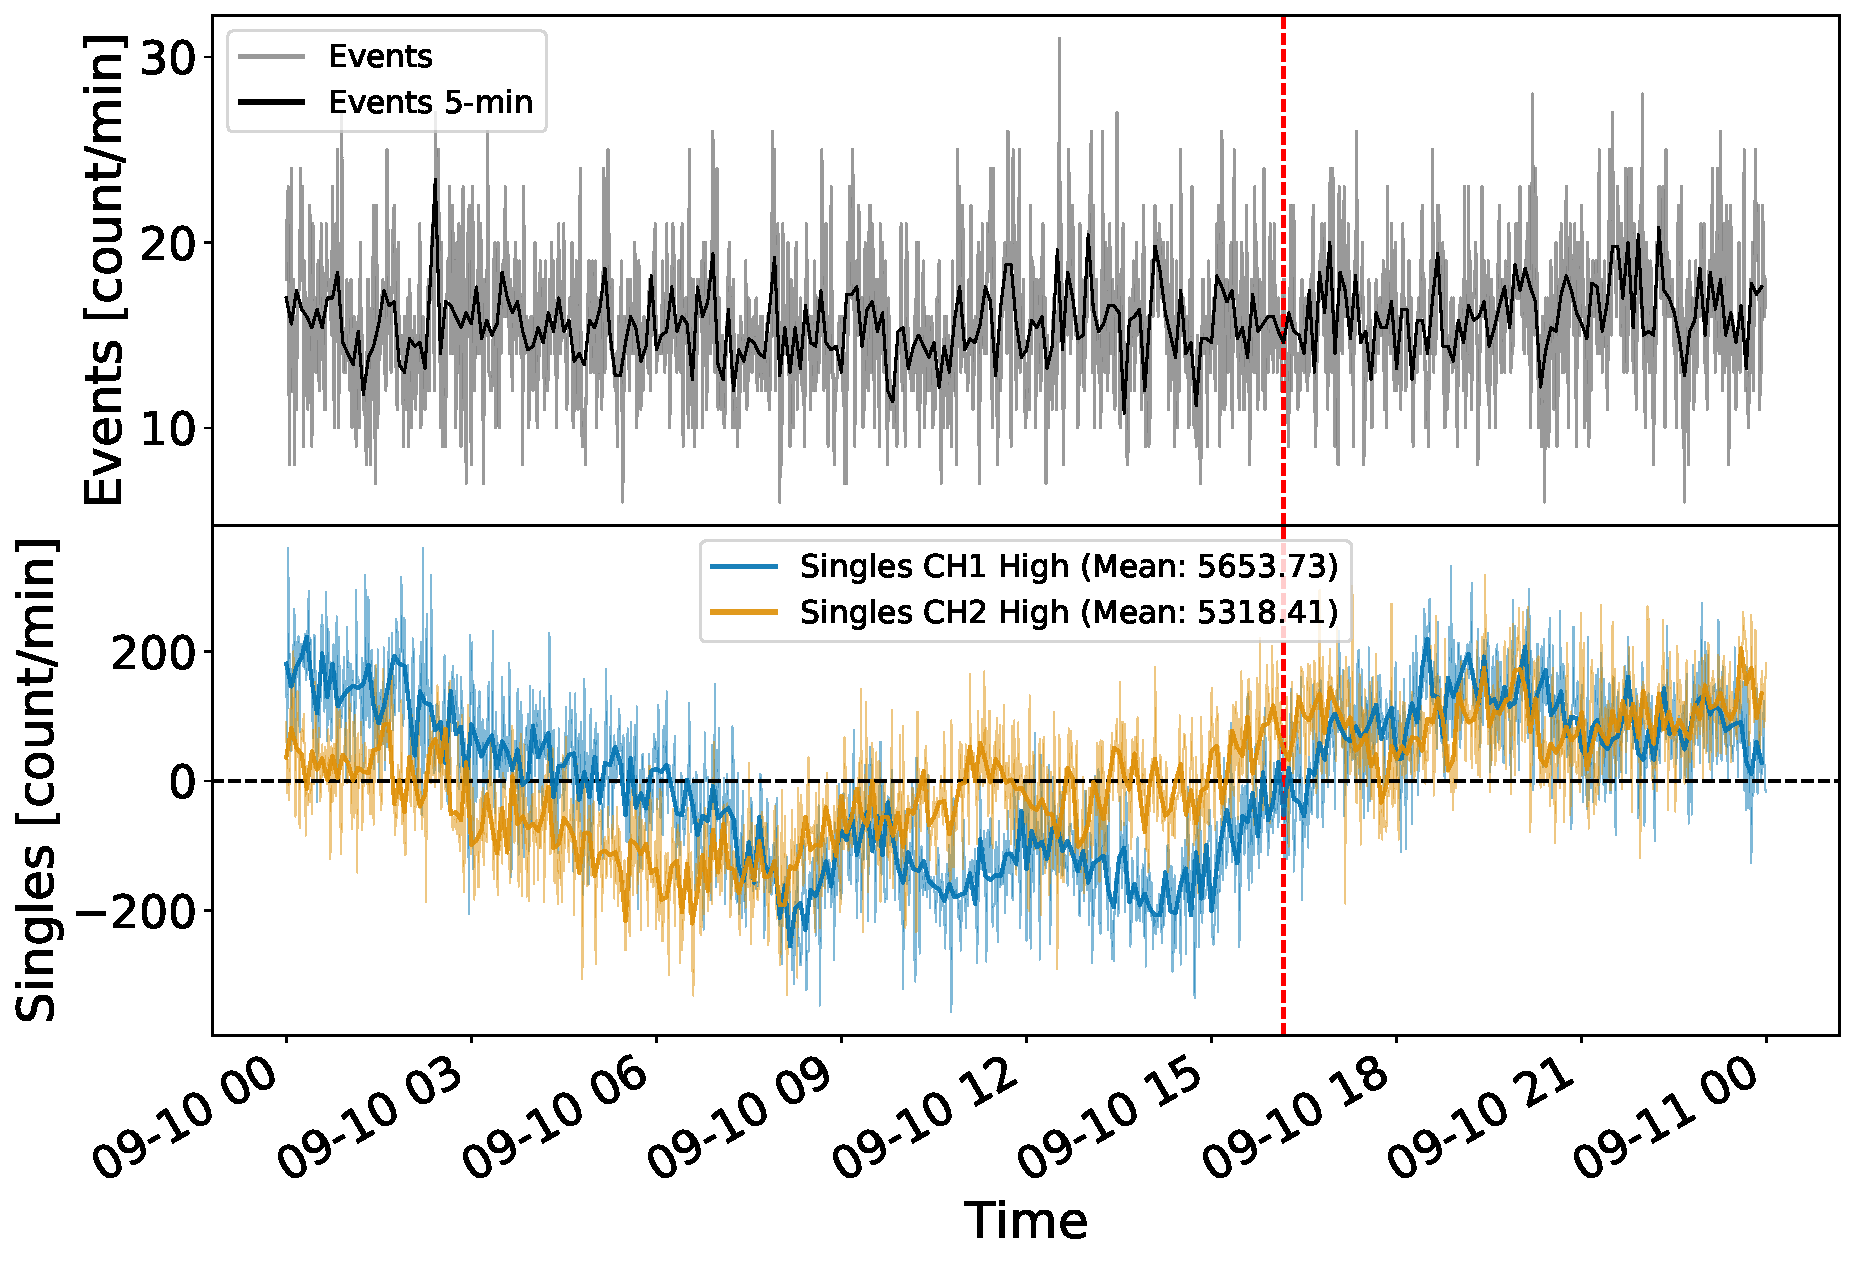
\includegraphics[width=0.48\columnwidth]{GLE72_203.pdf}
		\label{fig:GLE72_203}} \\
	
	\qquad
	
	\subfloat[HS 8001 (Eindhoven)]{
		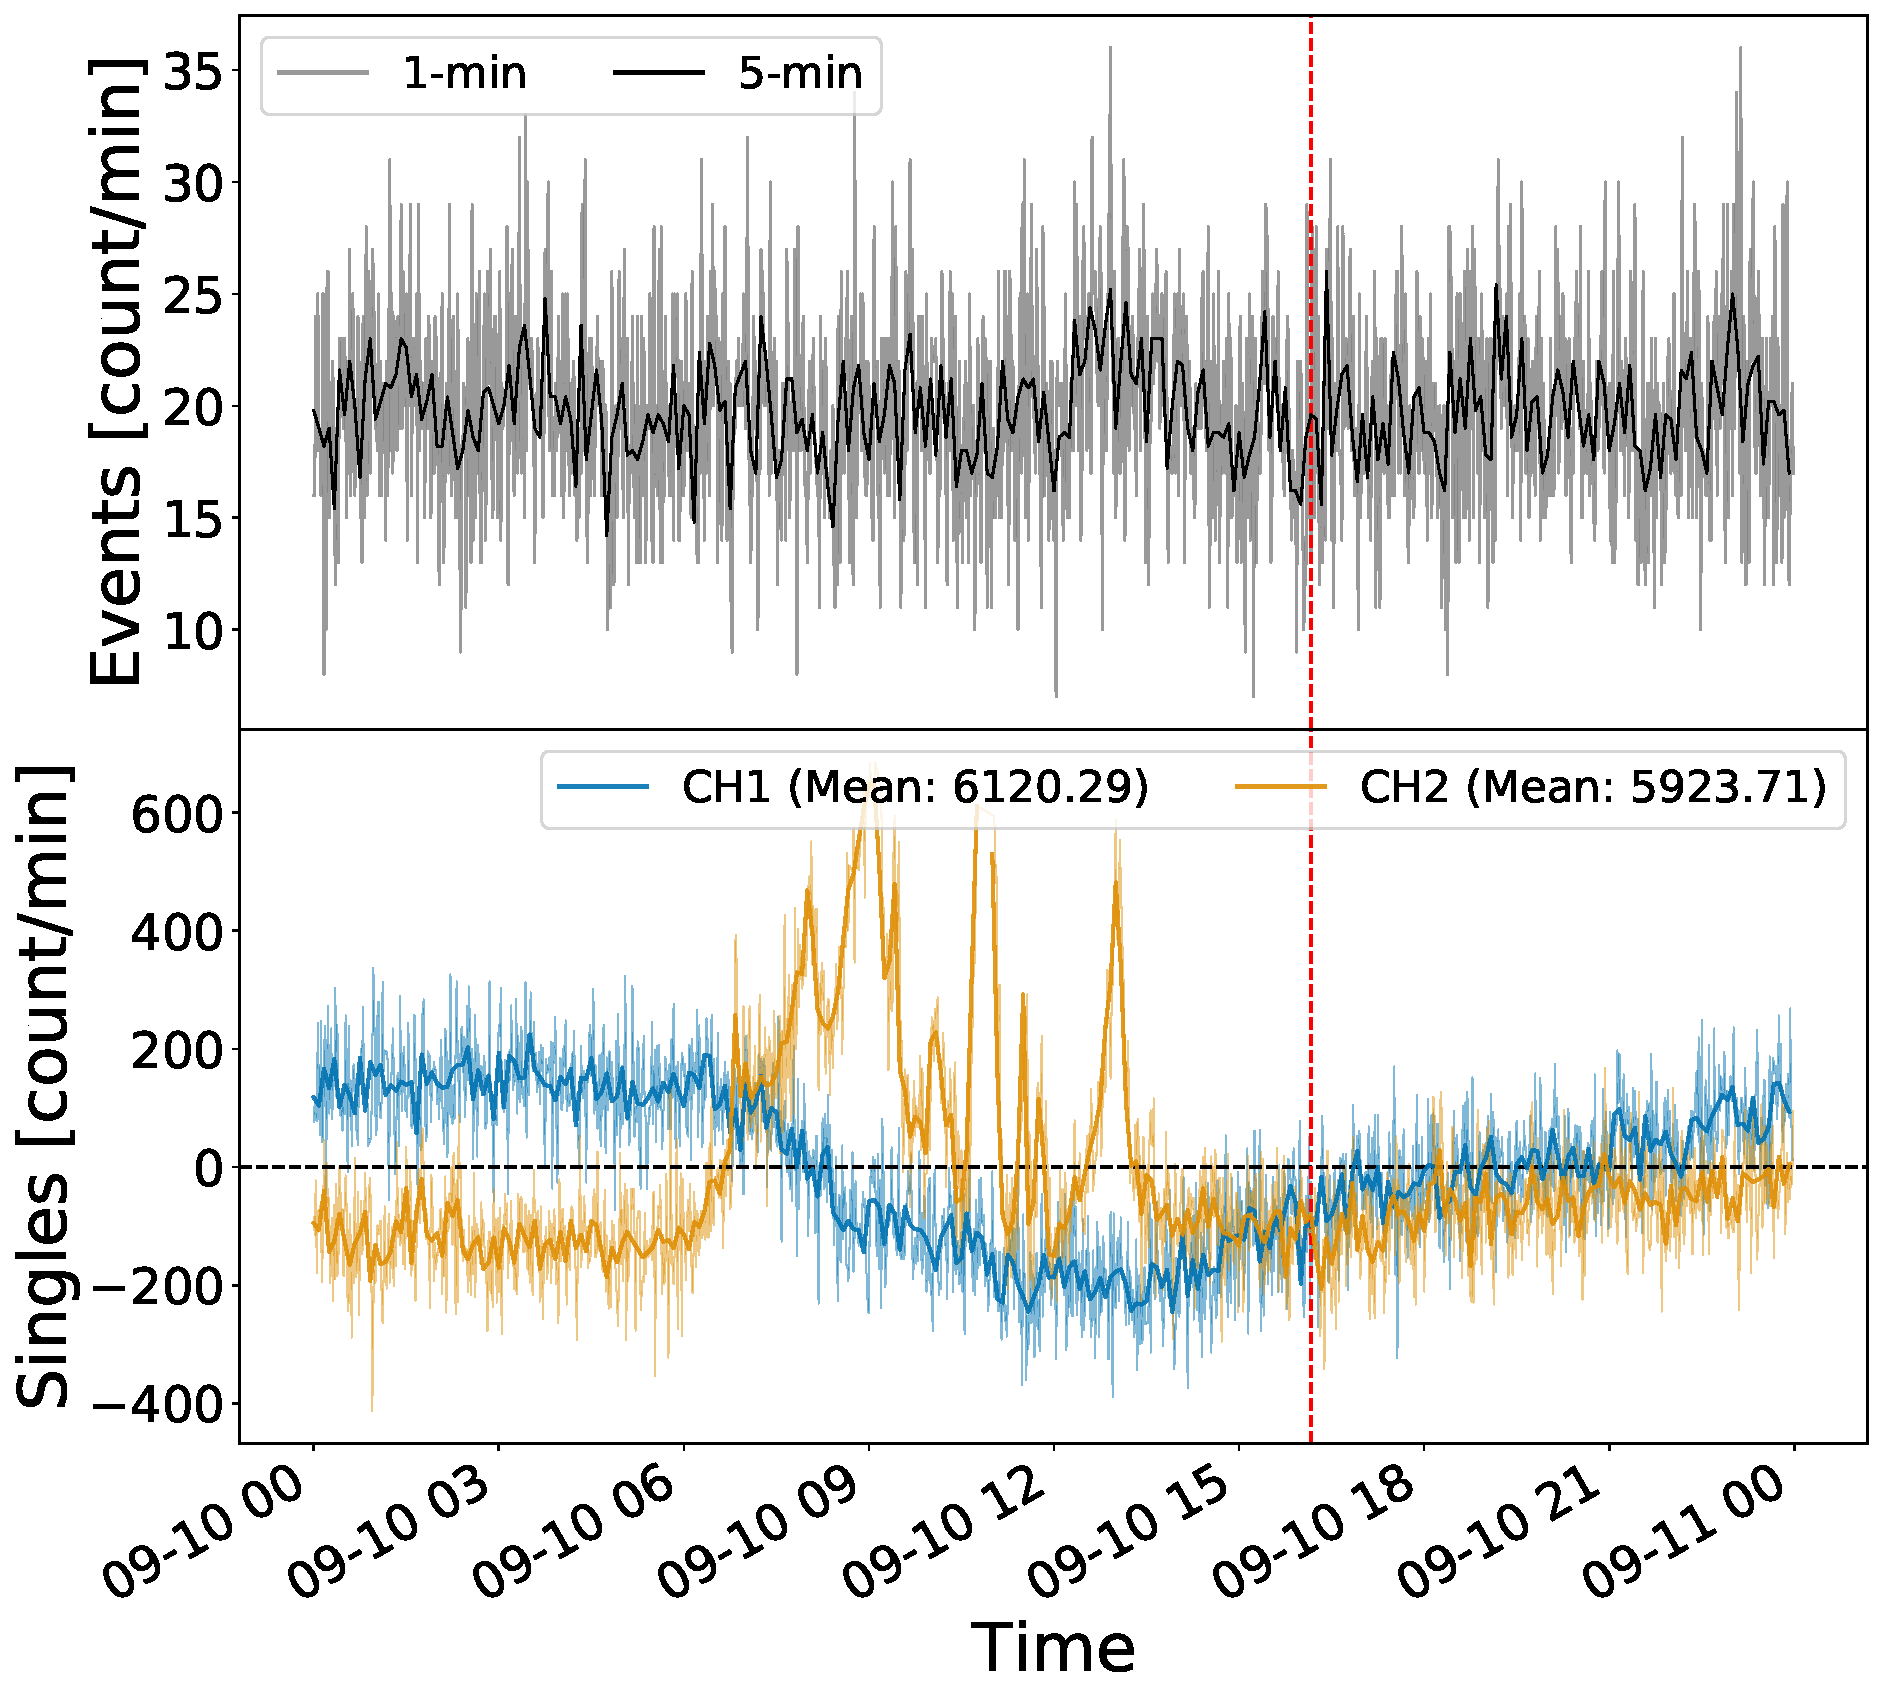
\includegraphics[width=0.48\columnwidth]{GLE72_8001.pdf}
		\label{fig:GLE72_8001}}
	%\qquad
	\subfloat[HS 14001 (Birmingham University)]{
		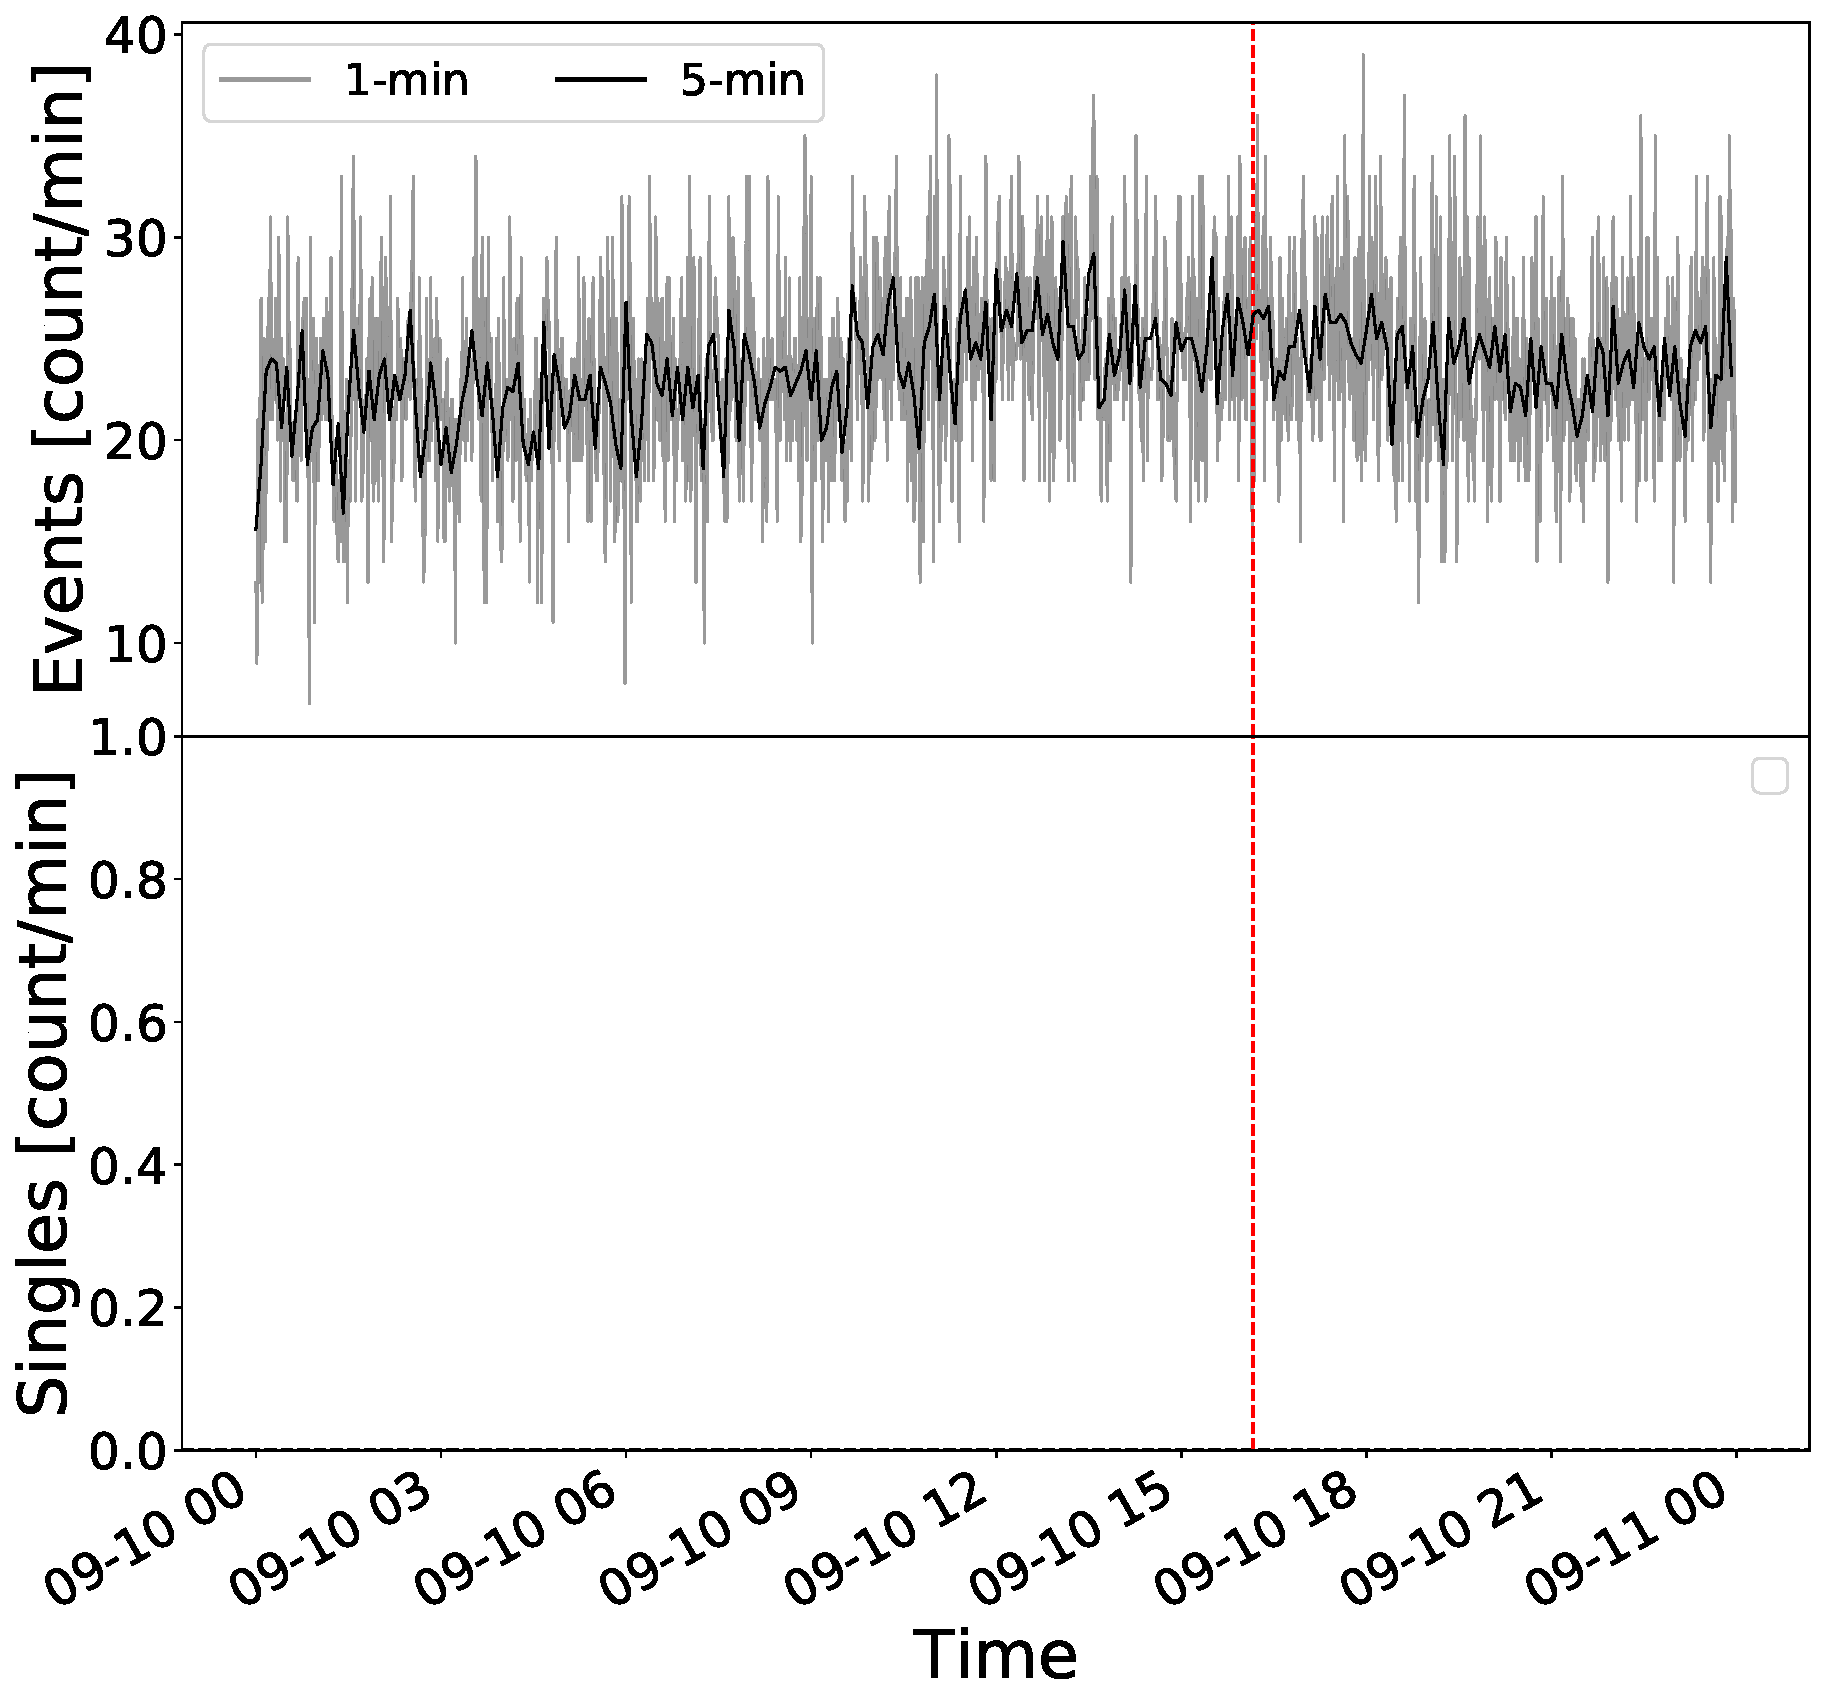
\includegraphics[width=0.48\columnwidth]{GLE72_14001.pdf}
		\label{fig:GLE72_14001}}
	
	\caption{HiSPARC data for 4 stations around the epoch of GLE 72. The top panel of each subplot shows the minute-averaged trigger events between detectors within the station, while the bottom panel shows the mean-shifted, minute-averaged counts by each individual detector in the station. The vertical red, dashed line depicts the approximate onset time of the GLE. The units of time on the x-axis are, MM-DD HH.}
	\label{fig:GLE_72}
\end{figure}


We can see from Figures~\ref{fig:GLE_70},~\ref{fig:GLE_71}, and~\ref{fig:GLE_72} that there are no clear and obvious signs of the \gls{gle} signals in the HiSPARC observations. This is the case for both the events data and the singles data.

There are some excursions from the mean count rate, this is significantly more prominent in the singles rates which are shown in the \gls{gle} 72 plots for stations 501, 203, and 8001. It is believed that these excursions are the effect of atmospheric pressure on the muon count rates; in Section~\ref{sec:HS_standardisation} this is discussed further and is accounted for.

No clear \glspl{gle} have been observed in the HiSPARC data. We believe this is due to the rigidity cut-off of the HiSPARC stations, as \glspl{gle} are caused by \glspl{sep} with a lower energy. Typically \glspl{gle} are observed by \glspl{nm}, and only the most energetic have been observed by \glspl{md} [...(...(...cite to https://doi.org/10.1088/0004-637X/761/2/101 and maybe also to https://doi.org/10.1093/pasj/psv111...)...)...]. In Section~\ref{HS_standardisation} we investigated the \gls{cr} spectrum to infer our ability to measure \glspl{gle} with the HiSPARC stations. We do also note that the atmospheric effects in the raw do not help our ability to observe the space weather and these effects were later removed (see Section~\ref{sec:HS_P_corr}).


%%%%%%%%%%%%%%%%%%%%%%%%%%%%%%%%%%%%%%%%%%%%%%%%%%%%%%%%%%%%%%%%%%%%%
\subsection{HiSPARC Observations of Forbush Decreases}

%From \citet{lingri_forbush_2016}: "The majority of \gls{fd}s are produced by CMEs with velocities from 400 to 1200 km/sec and at the same time the velocity of the solar wind fluctuates from 400 to 740 km/sec"

The search for evidence of FDs within the HiSPARC data was conducted for the \glspl{fd} highlighted in Table~\ref{tab:space_weather_events}. Figure~\ref{fig:FD_201203}, Figure~\ref{fig:FD_201207}, and Figure~\ref{fig:FD_201412} show the HiSPARC observations around the epochs of the first four \glspl{fd} listed in Table~\ref{tab:space_weather_events}. Each of the plots shows only  observations using the HiSPARC events data (i.e. coincidences between the detectors of a station).

\begin{figure}[ht]
	\centering
	\subfloat[HS 501 (Nikhef)]{
		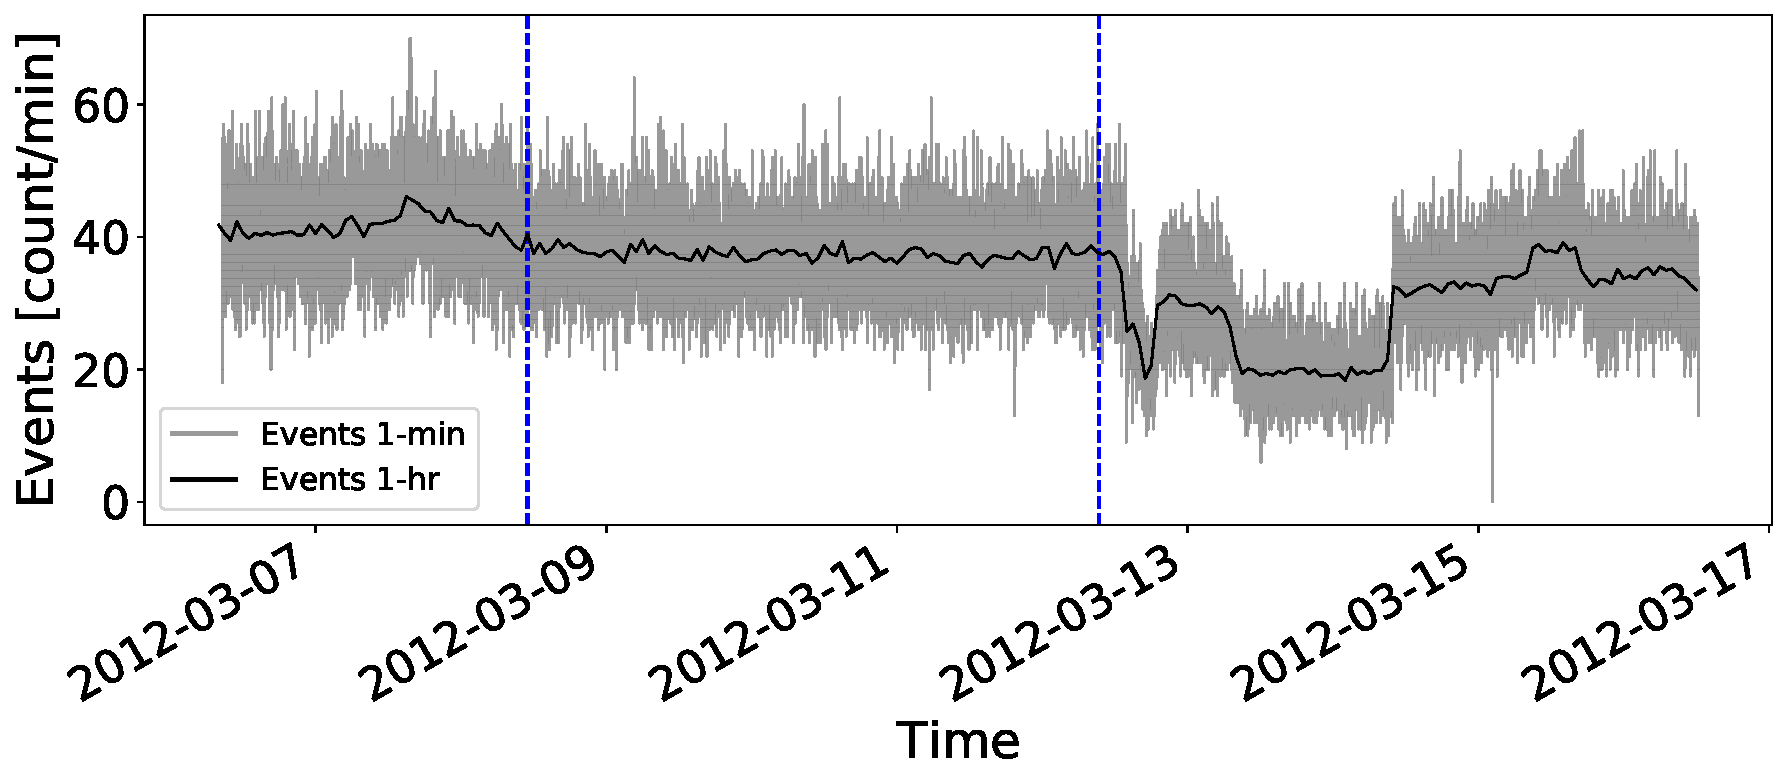
\includegraphics[width=0.48\columnwidth]{FD_201203_501.pdf}
		\label{fig:FD_201203_501}}
	%\qquad
	\subfloat[HS 8001 (Eindhoven)]{
		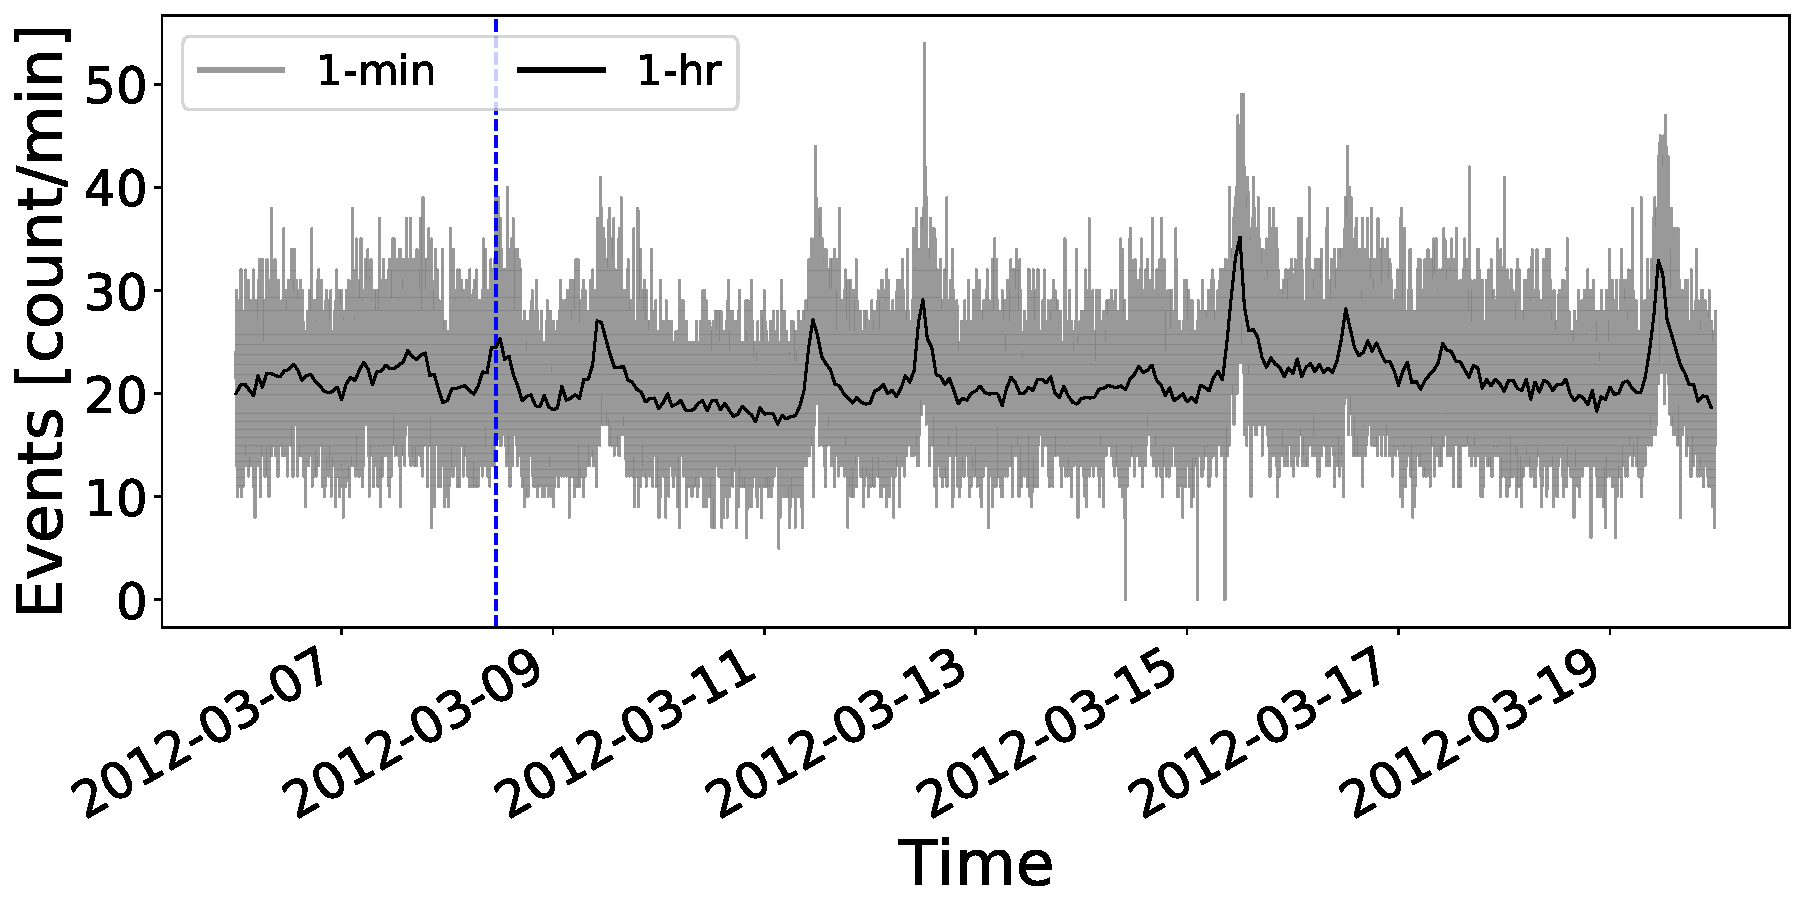
\includegraphics[width=0.48\columnwidth]{FD_201203_8001.pdf}
		\label{fig:FD_201203_8001}}
	
	\caption{HiSPARC data for stations 501 and 8001 around the epoch of the FDs in March 2012. The plot shows the minute-averaged and hourly-averaged trigger events between detectors within the station. The vertical blue-dashed lines show the approximate onset-time of the FDs. The units of time on the x-axis are, YYYY-MM-DD.}
	\label{fig:FD_201203}
\end{figure}

\begin{figure}[ht]
	\centering
	\subfloat[HS 501 (Nikhef)]{
		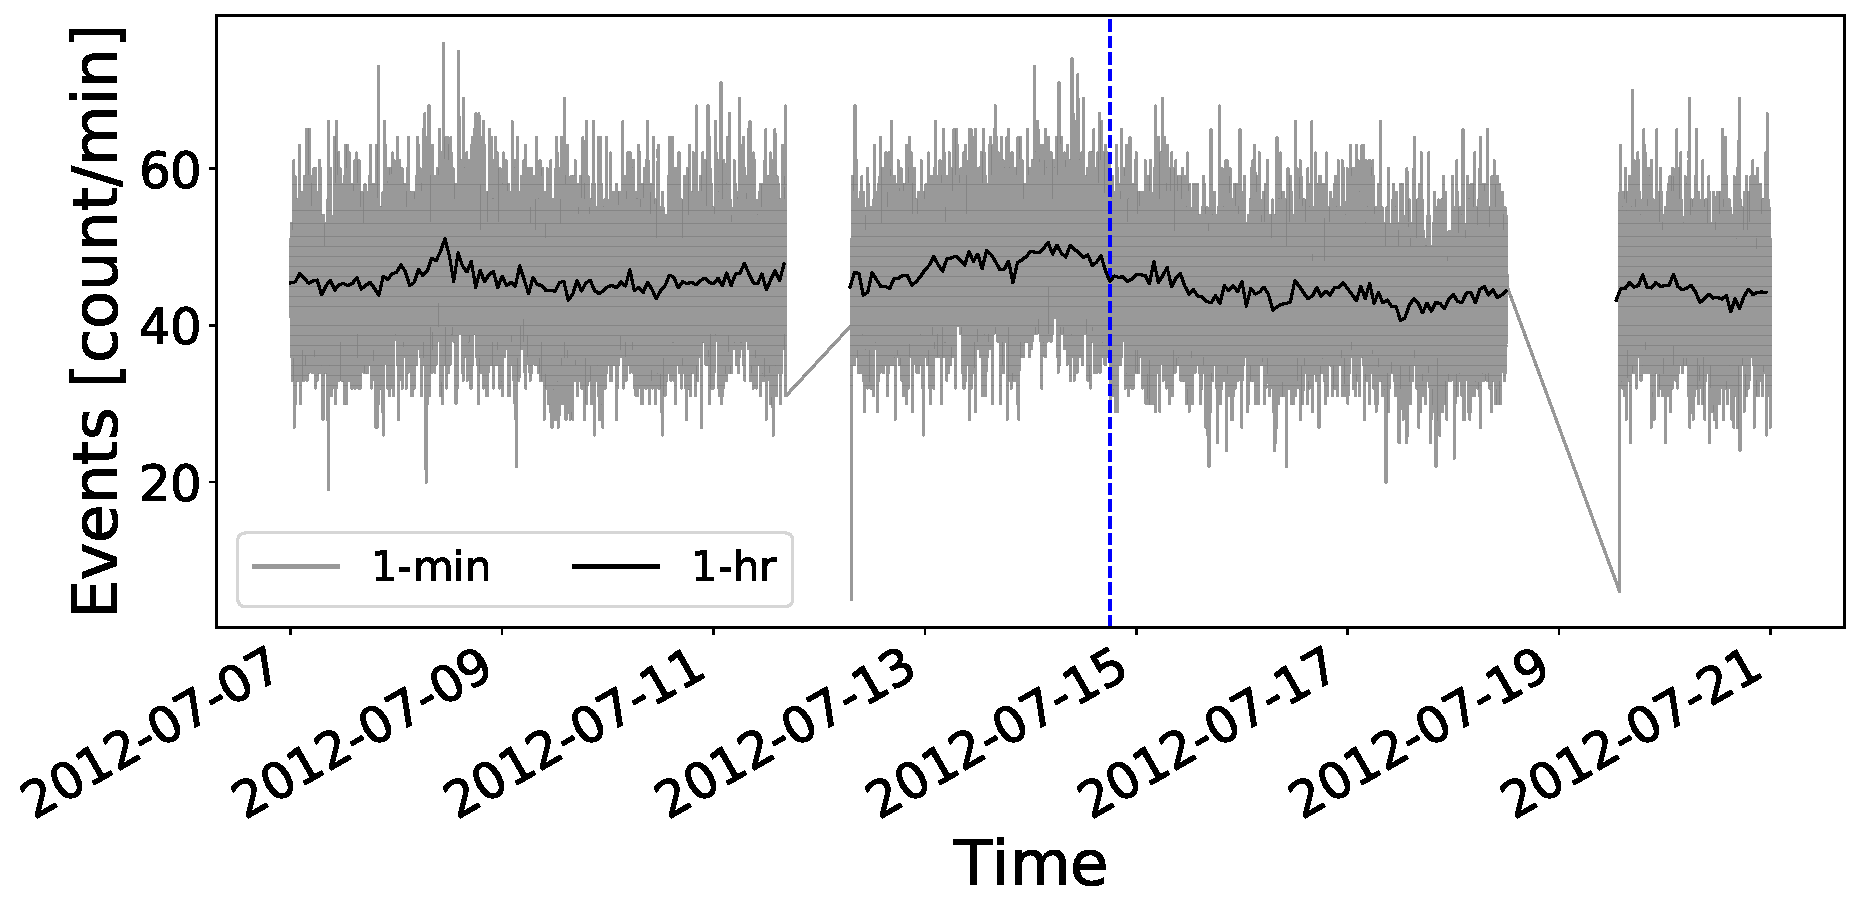
\includegraphics[width=0.48\columnwidth]{FD_201207_501.pdf}
		\label{fig:FD_201207_501}}
	%\qquad
	\subfloat[HS 8001 (Eindhoven)]{
		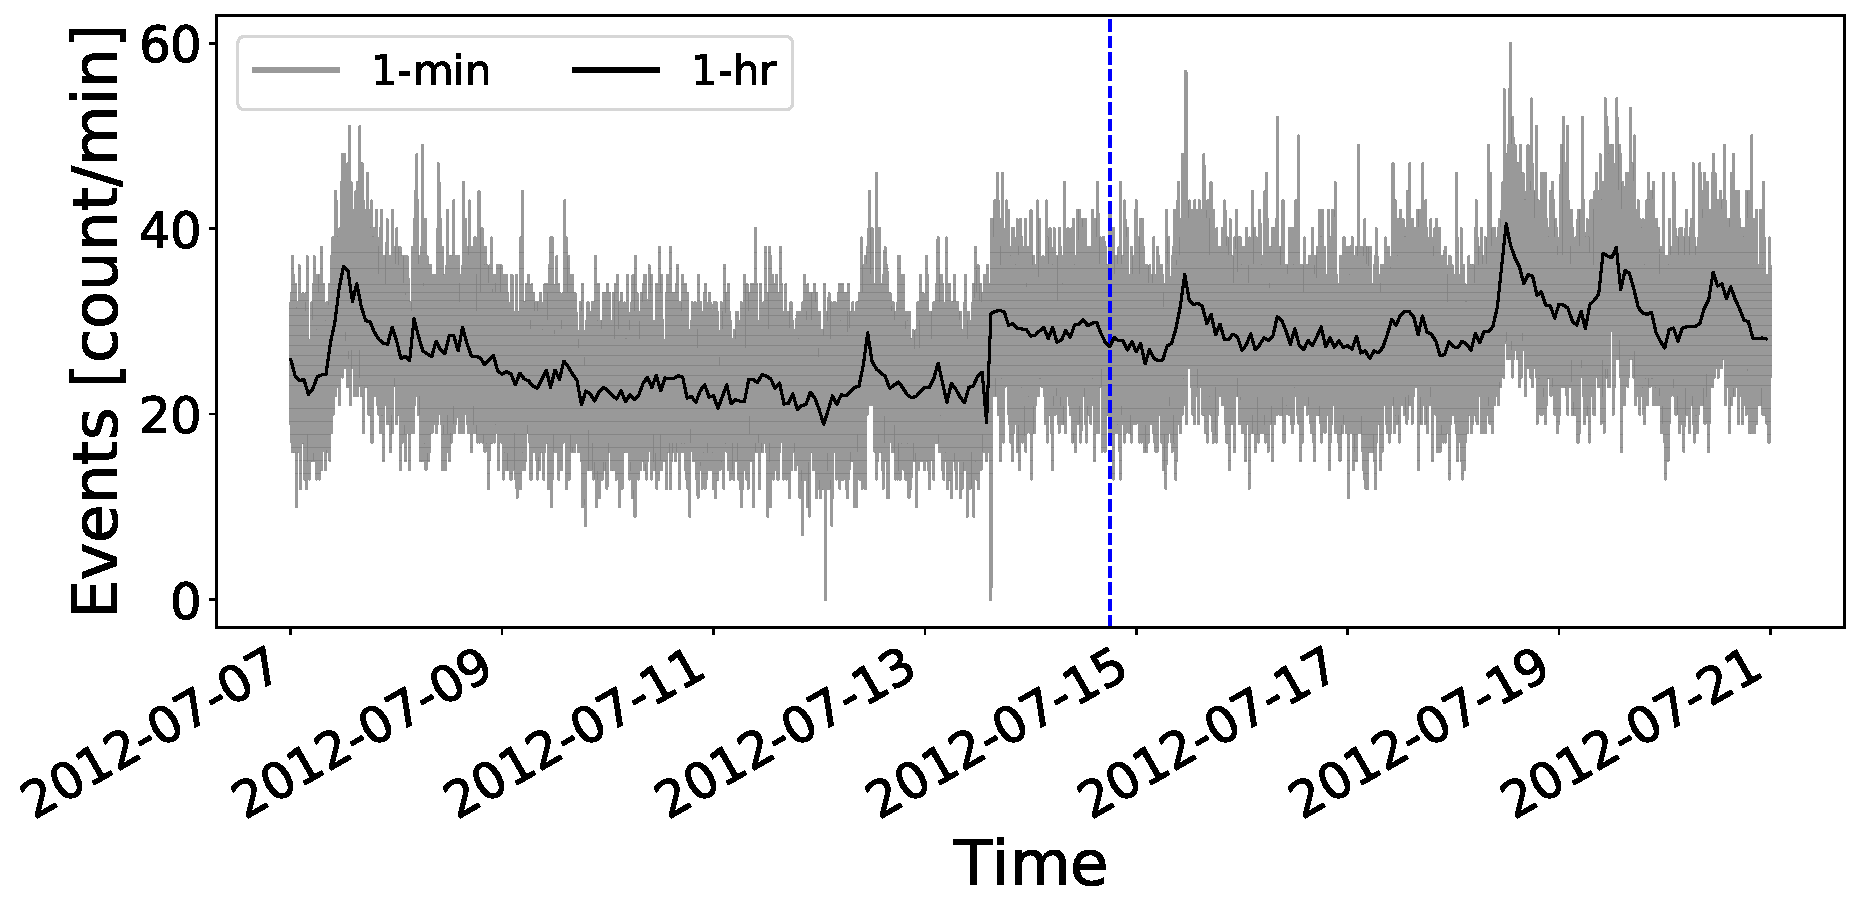
\includegraphics[width=0.48\columnwidth]{FD_201207_8001.pdf}
		\label{fig:FD_201207_8001}}
	
	\caption{HiSPARC data for stations 501 and 8001 around the epoch of the FD in July 2012. The plot shows the minute-averaged and hourly-averaged trigger events between detectors within the station. The vertical blue-dashed line shows the approximate onset-time of the FD. The units of time on the x-axis are, YYYY-MM-DD.}
	\label{fig:FD_201207}
\end{figure}

\begin{figure}[ht]
	\centering
	\subfloat[HS 501 (Nikhef)]{
		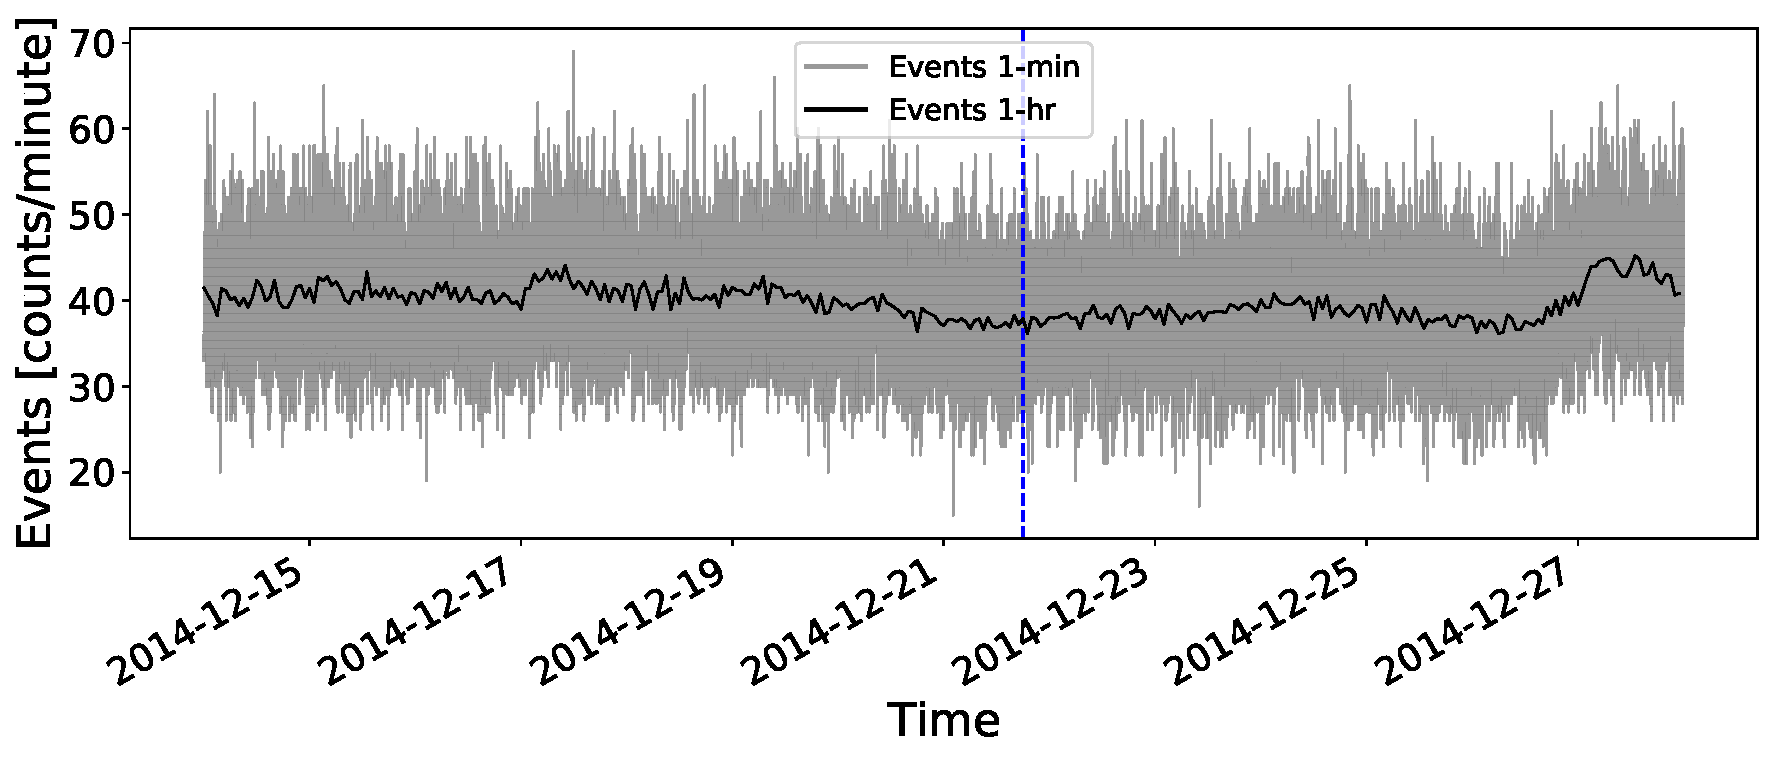
\includegraphics[width=0.48\columnwidth]{FD_201412_501.pdf}
		\label{fig:FD_201412_501}}
	%\qquad
	\subfloat[HS 203 (College Hageveld)]{
		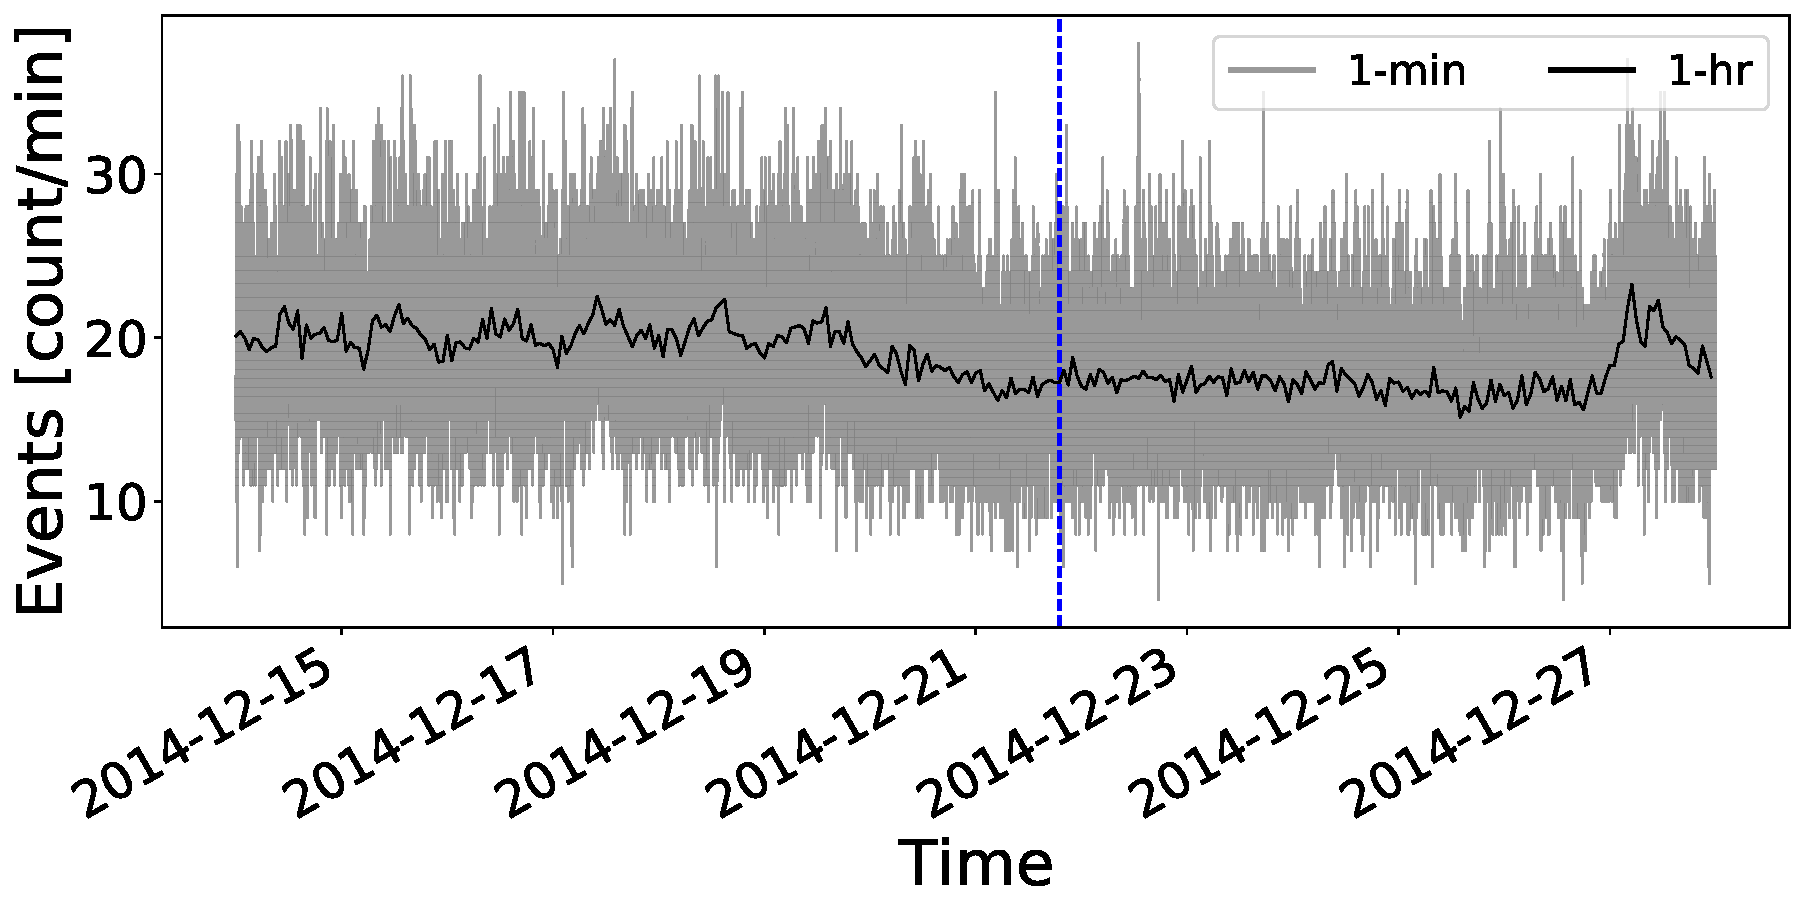
\includegraphics[width=0.48\columnwidth]{FD_201412_203.pdf}
		\label{fig:FD_201412_203}} \\
	
	\qquad
	
	\subfloat[HS 3001 (Leiden)]{
		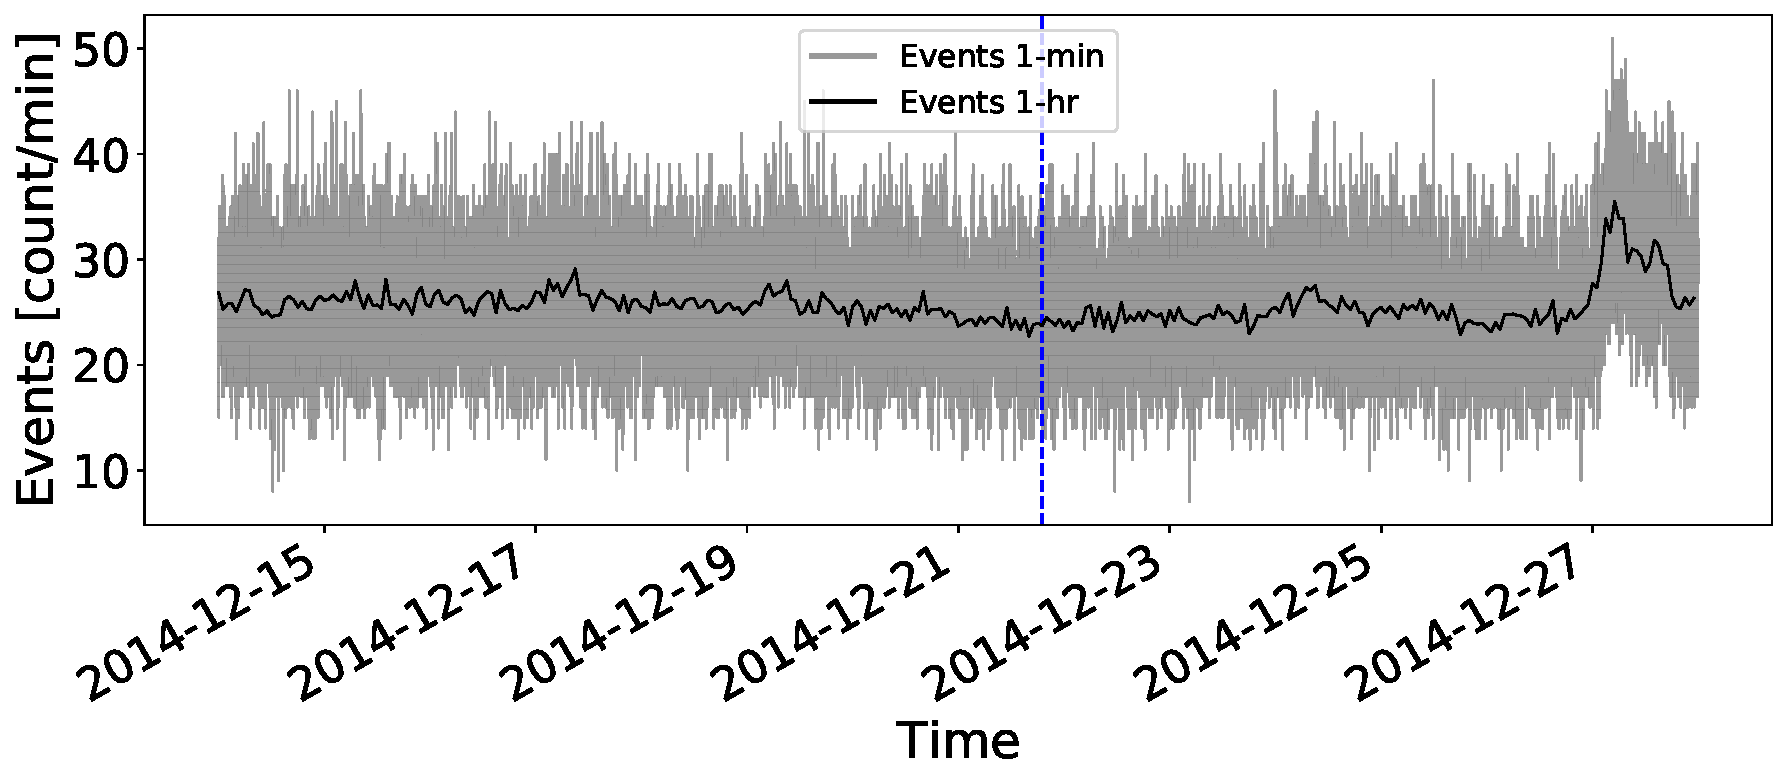
\includegraphics[width=0.48\columnwidth]{FD_201412_3001.pdf}
		\label{fig:FD_201412_3001}}
	%\qquad
	\subfloat[HS 14001 (Birmingham University)]{
		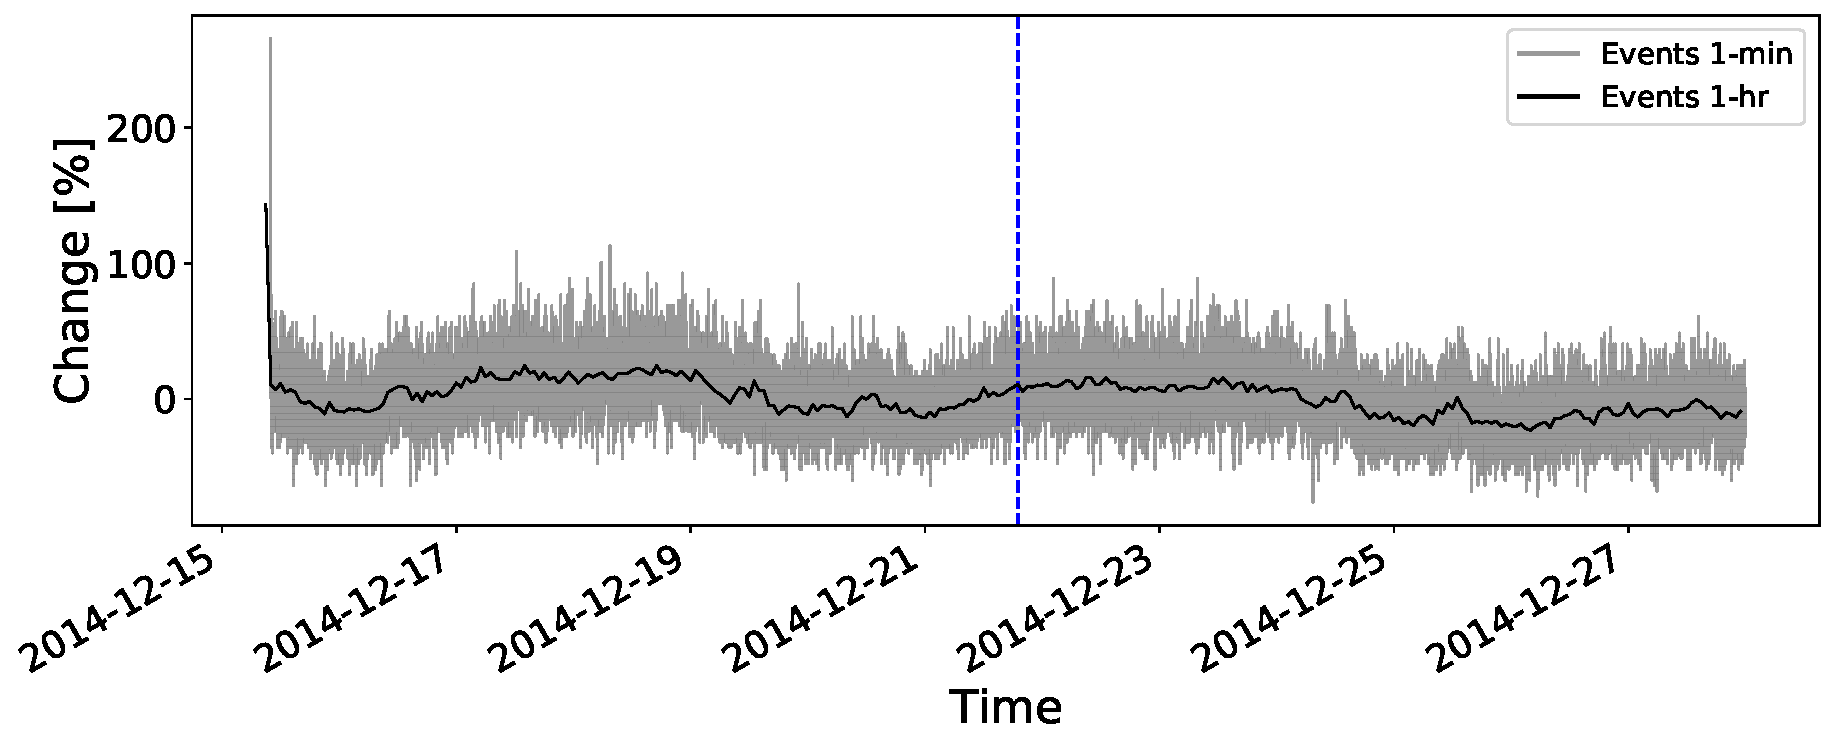
\includegraphics[width=0.48\columnwidth]{FD_201412_14001.pdf}
		\label{fig:FD_201412_14001}}
	
	\caption{HiSPARC data for four stations around the epoch of the FD in December 2014. The plot shows the minute-averaged and hourly-averaged trigger events between detectors within the station. The vertical blue-dashed line shows the approximate onset-time of the FD. The units of time on the x-axis are, YYYY-MM-DD.}
	\label{fig:FD_201412}
\end{figure}


We can see from the plots that there are no clear signs of the anticipated \gls{fd} signals in the HiSPARC observations. We observed a set of significant decreases in the muon count rate in station 501 after the second \gls{fd} in March 2012 (see Figure~\ref{fig:FD_201203_501}); however, it is unclear whether this is a consequence of the \gls{fd} or other, hardware reasons, as the \gls{fd} was not observed in the other HiSPARC station. The shape of the \gls{fd} in the \gls{nm} data shows a sudden decrease and a smooth recovery within two days, but the shape of the HiSPARC data shows a more complicated effect, which suggests that the cause is not the \gls{fd}, but rather a result of hardware.

In the other station we also observe some variations in the count rate which vary over longer time scales, but this is due to variations in the atmospheric pressure. Note that this needs accounting for and comes later...

It is quite clear from Figure~\ref{fig:FD_201203_8001} and Figure~\ref{fig:FD_201207_8001} that stations 8001 (Eindhoven) displays a semi-persistent diurnal variation in the count rate...

For the final two \glspl{fd} listed in Table~\ref{tab:space_weather_events}, the plot of the HiSPARC observations is shown in Figure~\ref{fig:FD_GLE72}. Plotted are the HiSPARC events data, and where possible, we also show the singles rates from each of the individual detectors in a station when the singles rate data is available. Furthermore, as these \glspl{fd} were precursory to \gls{gle}72, we also marked on the epoch of the \gls{gle} for completeness.

\begin{figure}[ht]
	\centering
	\subfloat[HS 501 (Nikhef)]{
		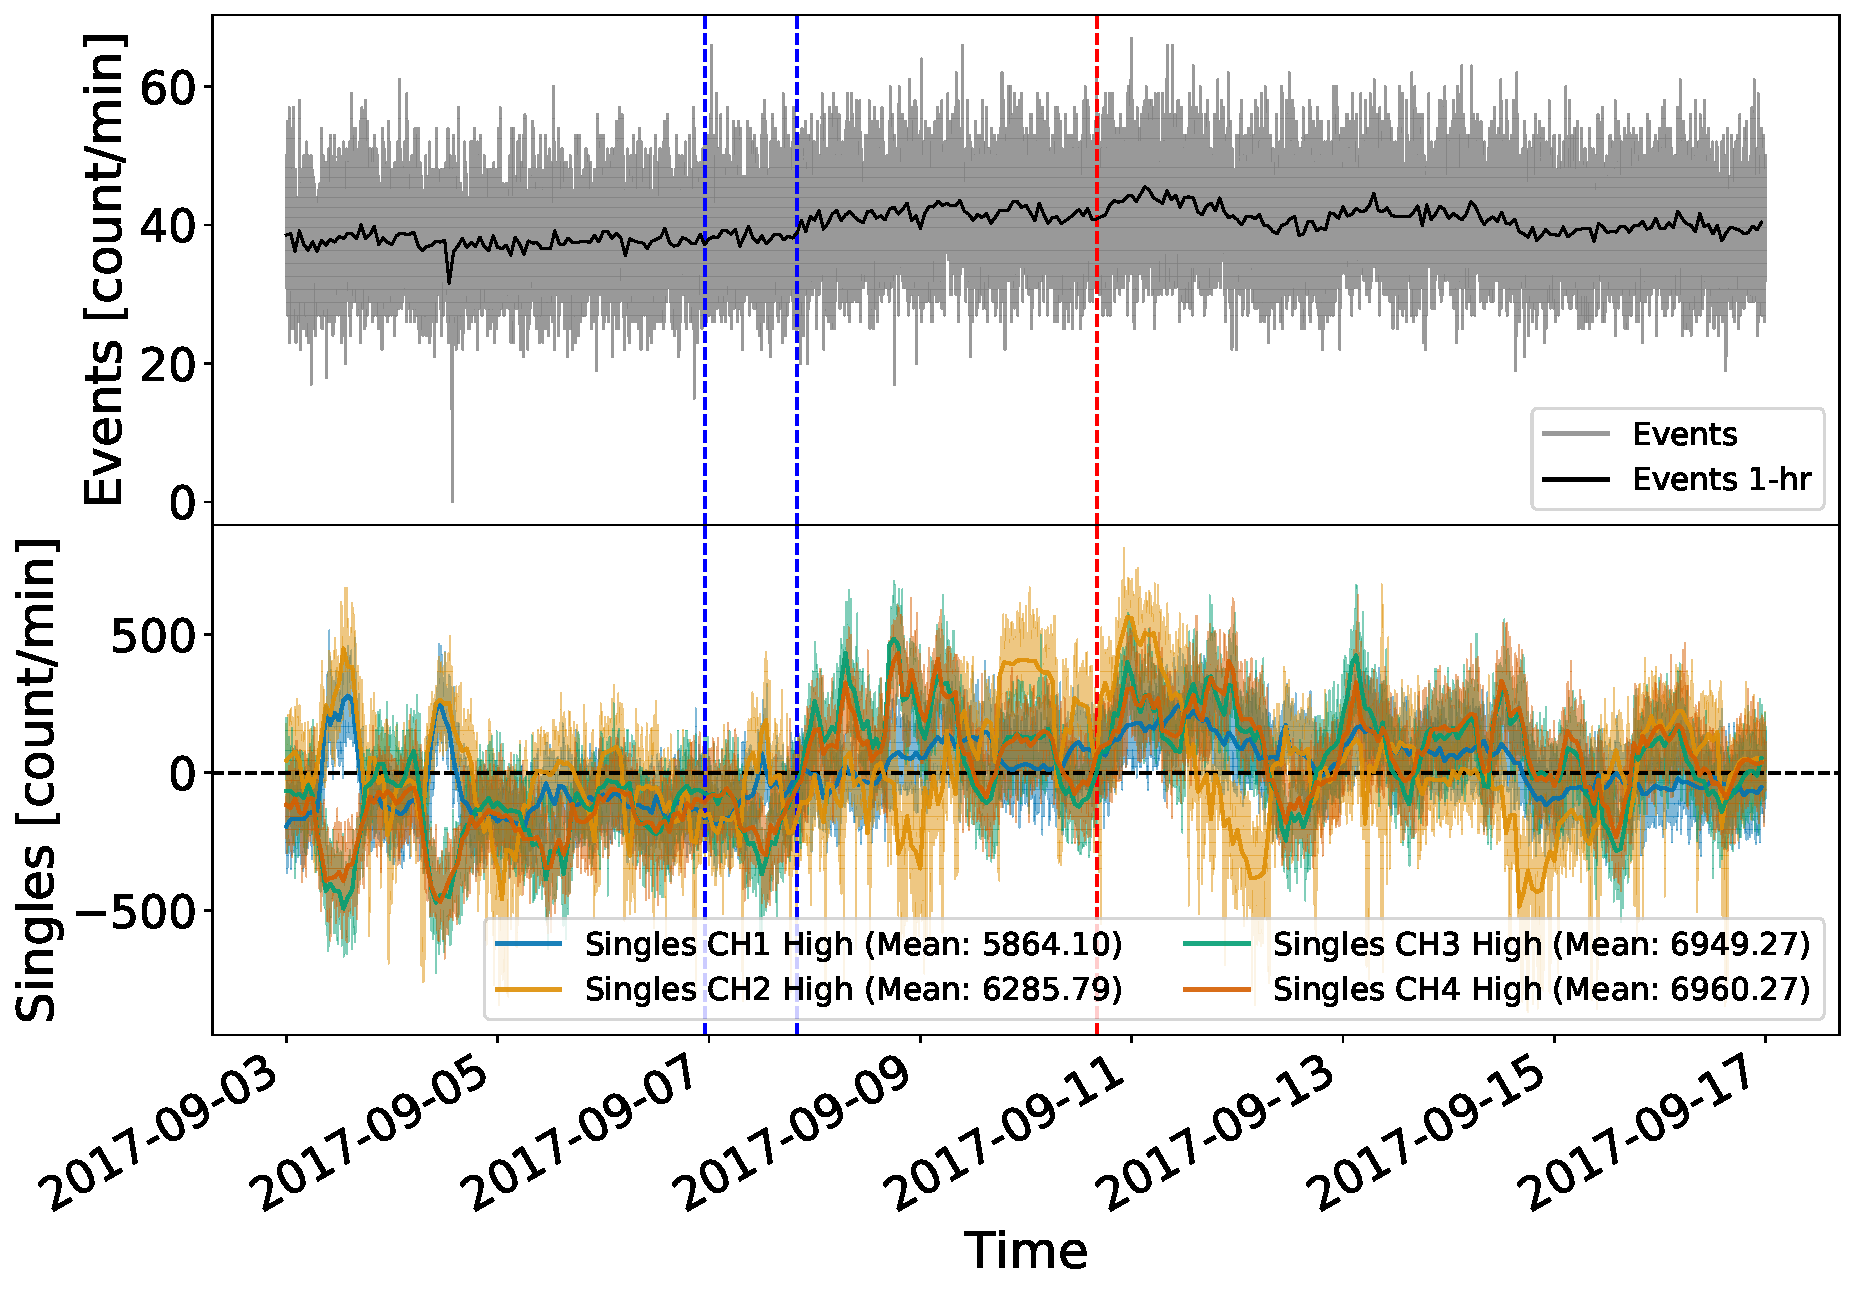
\includegraphics[width=0.48\columnwidth]{FD_GLE72_501.pdf}
		\label{fig:FD_GLE72_501}}
	%\qquad
	\subfloat[HS 203 (College Hageveld)]{
		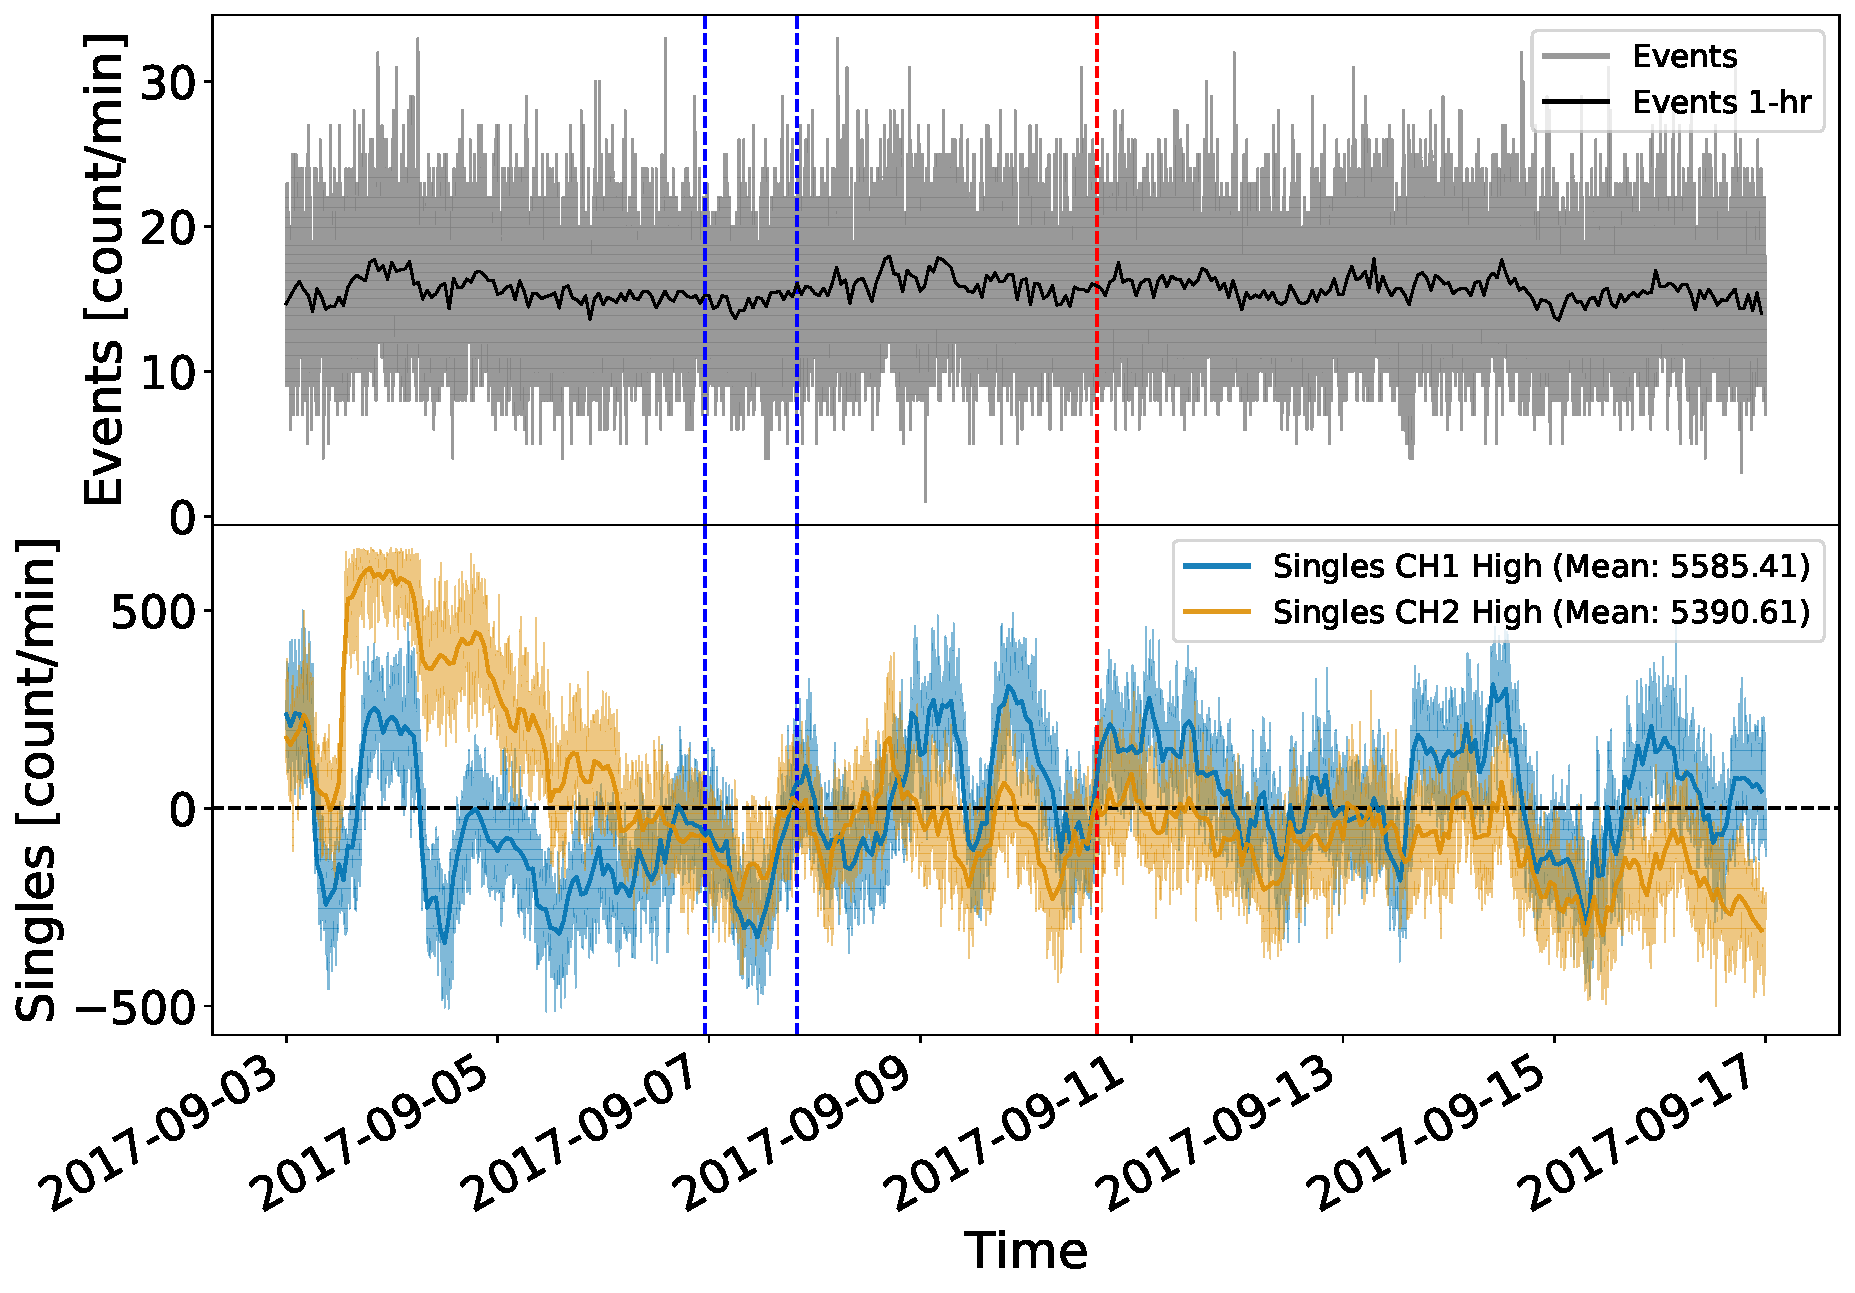
\includegraphics[width=0.48\columnwidth]{FD_GLE72_203.pdf}
		\label{fig:FD_GLE72_203}} \\
	
	\qquad
	
	\subfloat[HS 8001 (Eindhoven)]{
		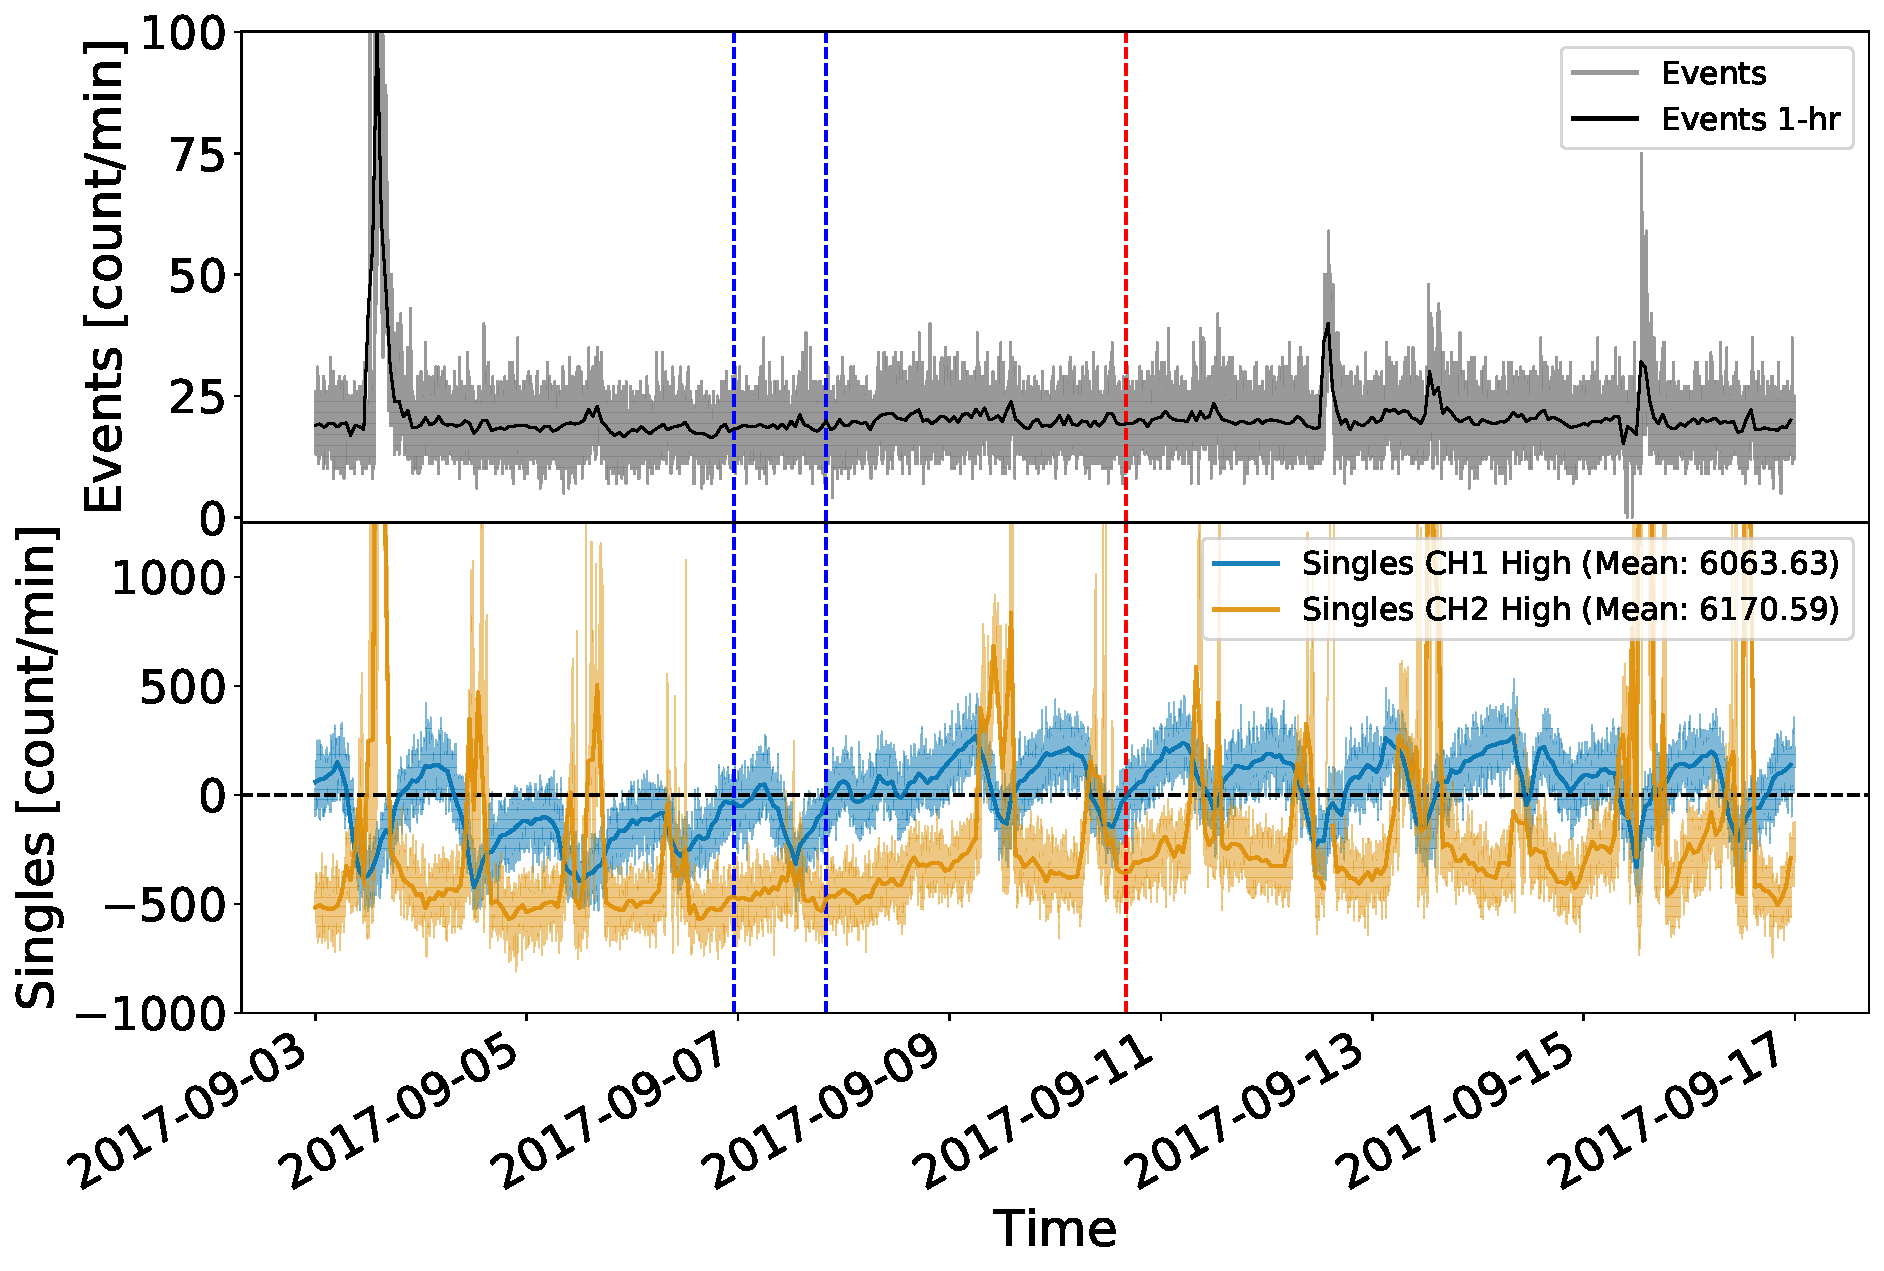
\includegraphics[width=0.48\columnwidth]{FD_GLE72_8001.pdf}
		\label{fig:FD_GLE72_8001}}
	%\qquad
	\subfloat[HS 14001 (Birmingham University)]{
		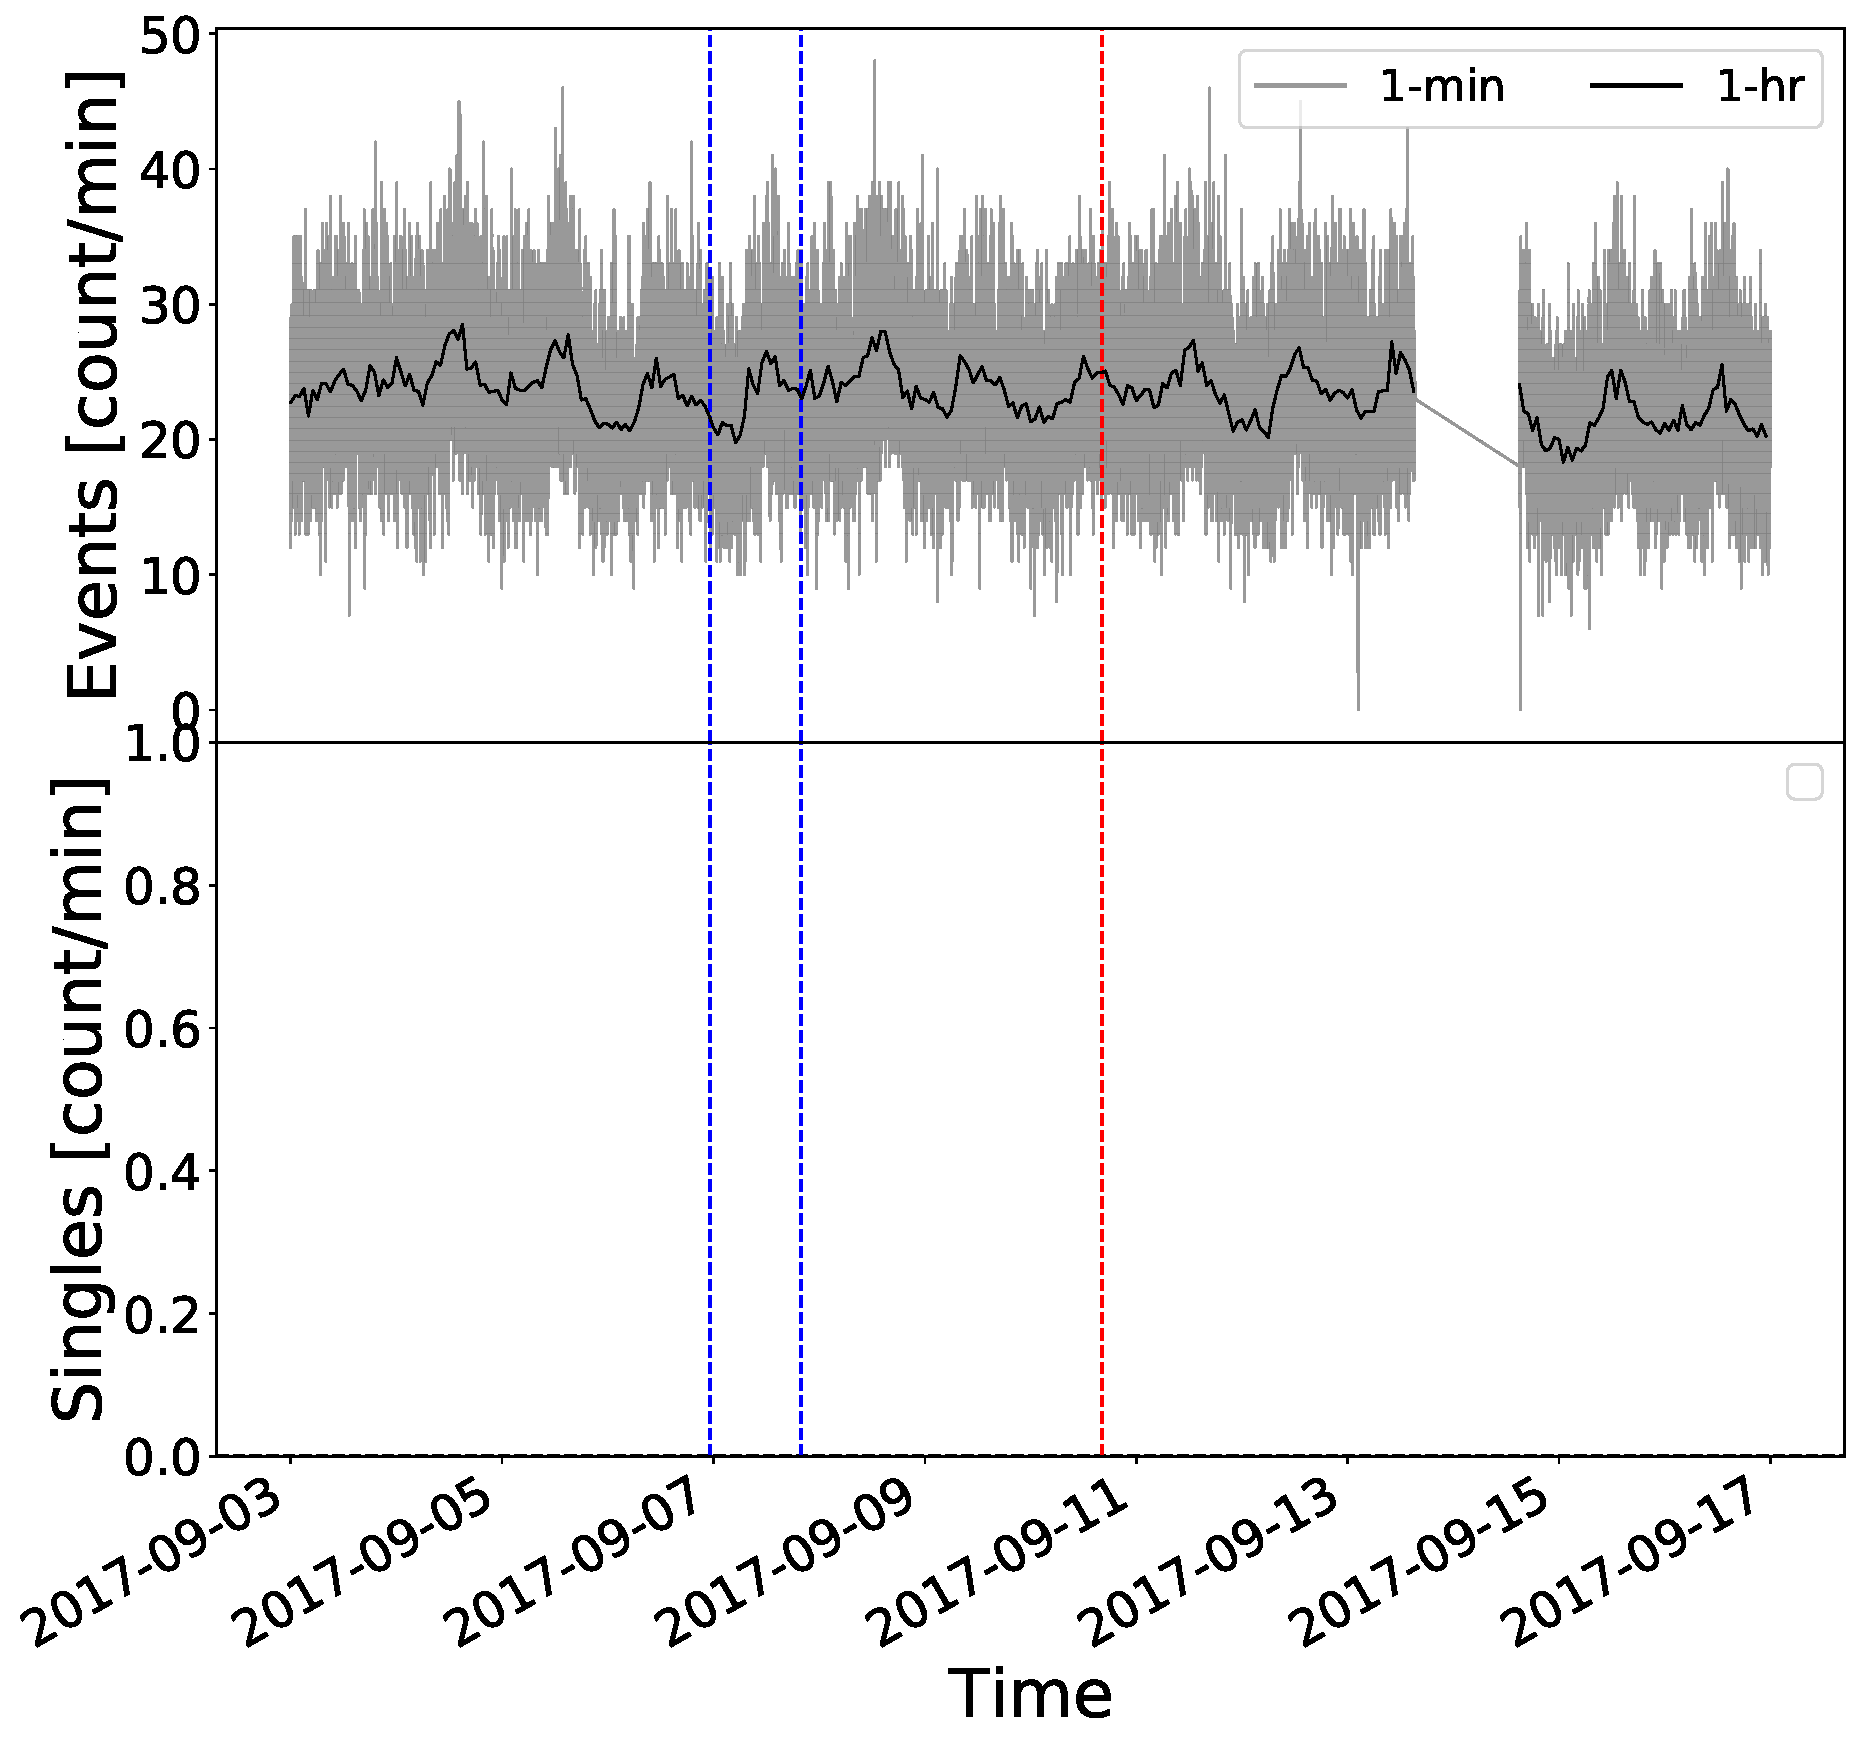
\includegraphics[width=0.48\columnwidth]{FD_GLE72_14001.pdf}
		\label{fig:FD_GLE72_14001}}
	
	\caption{HiSPARC data for four stations around the epoch in which there were several FDs close to the onset of GLE 72. The top panel of each subplot shows the minute-averaged trigger events between detectors within the station, while the bottom panel shows the mean-shifted, minute-averaged counts by each individual detector in the station. The vertical blue-dashed lines show the approximate onset-times of the two FDs observed around this epoch and the red-dashed line depicts the approximate onset time of the GLE. The units of time on the x-axis are, YYYY-MM-DD.}
	\label{fig:FD_GLE72}
\end{figure}

As with the other \gls{fd} epochs, we again do not observe any clear signs of the \gls{fd} signals in either the events or singles data. In each of the three stations for which there was singles data, we observed the semi-persistent diurnal signal, and again in the events for stations 14001. Furthermore, we also observed a similar slower variation in the count rate which is due to atmospheric pressure and needs to be accounted for.

No clear signal of \glspl{fd} has been observed in the raw HiSPARC data. We again believe this could be due to the rigidity cut-off of the HiSPARC stations. We also note that the atmospheric effects in the raw do not help our ability to observe the space weather and these effects were later removed (see Section~\ref{sec:HS_P_corr}). 



%%%%%%%%%%%%%%%%%%%%%%%%%%%%%%%%%%%%%%%%%%%%%%%%%%%%%%%%%%%%%%%%%%%%%
%%%%%%%%%%%%%%%%%%%%%%%%%%%%%%%%%%%%%%%%%%%%%%%%%%%%%%%%%%%%%%%%%%%%%
\section{Air Shower Simulations}\label{sec:CORSIKA}

In order to understand the muon abundance and the scale of the footprints of air showers produced by \glspl{pcr}, simulations of air shower developments were performed for a range of \glspl{pcr} energies for both primary protons and $\alpha$-particles.

To simulate the \gls{cr} air shower development, the \gls{corsika} software was employed: a Monte Carlo programme providing detailed simulations of the evolution of air showers initiated by \glspl{pcr} through the atmosphere \citep{heck_extensive_2017}. The particles in the \gls{corsika} simulations are tracked through the atmosphere until they undergo interactions with atmospheric nuclei, decay due to their instability, or reach the ground level defined as the simulation terminator.

Proton and $\alpha$-particle initiated air showers were generated with energies ranging from $10^{9}$ to $10^{20}$~eV, and $4\times10^{9}$ to $10^{20}$~eV, respectively. In total $\sim 2\times10^5$ proton-initiated showers were simulated and $\sim 2\times10^5$ $\alpha$-particle-initiated air showers were simulated. The lists detailing the breakdown of \gls{pcr} energies and number of simulations is provided in Appendix~\ref{app:CORSIKA_sims}, along with a brief discussion of the settings chosen within the simulations.


%%%%%%%%%%%%%%%%%%%%%%%%%%%%%%%%%%%%%%%%%%%%%%%%%%%%%%%%%%%%%%%%%%%%%
\subsection{Air Shower Footprints}\label{sec:CORSIKA_footprint}

The average footprint of muons at ground level was acquired from the output \gls{corsika} simulations by taking the distribution of the muons at ground level at the end of the simulation as a function of their distance from the shower core. This was achieved for each individual simulation realisation, and for a given \gls{pcr} energy, the average footprint distribution was calculated by combining all of the individual simulation realisations. Figure~\ref{fig:shower_footprints} shows the distributions for air showers induced by vertically incident protons and $\alpha$-particles.

We also repeated the simulations for air showers randomly selected from a uniform distribution of incident angles between 0$^\circ$ (vertical) and 70$^\circ$, to provide a more representative simulation. Similar plots were produced to those in Figure~\ref{fig:shower_footprints}, but they are not shown here, as the difference is not drastically different by-eye.

%[Discuss how distance between the HiSPARC station 2d/4d detectors will impact the ability to view certain PCR energies, and sets an lower limit on the energies observable in the standard trigger mode]

\begin{figure}[ht!]
	\centering
	\subfloat[Proton initiated air shower. \label{fig:p_footprint}]{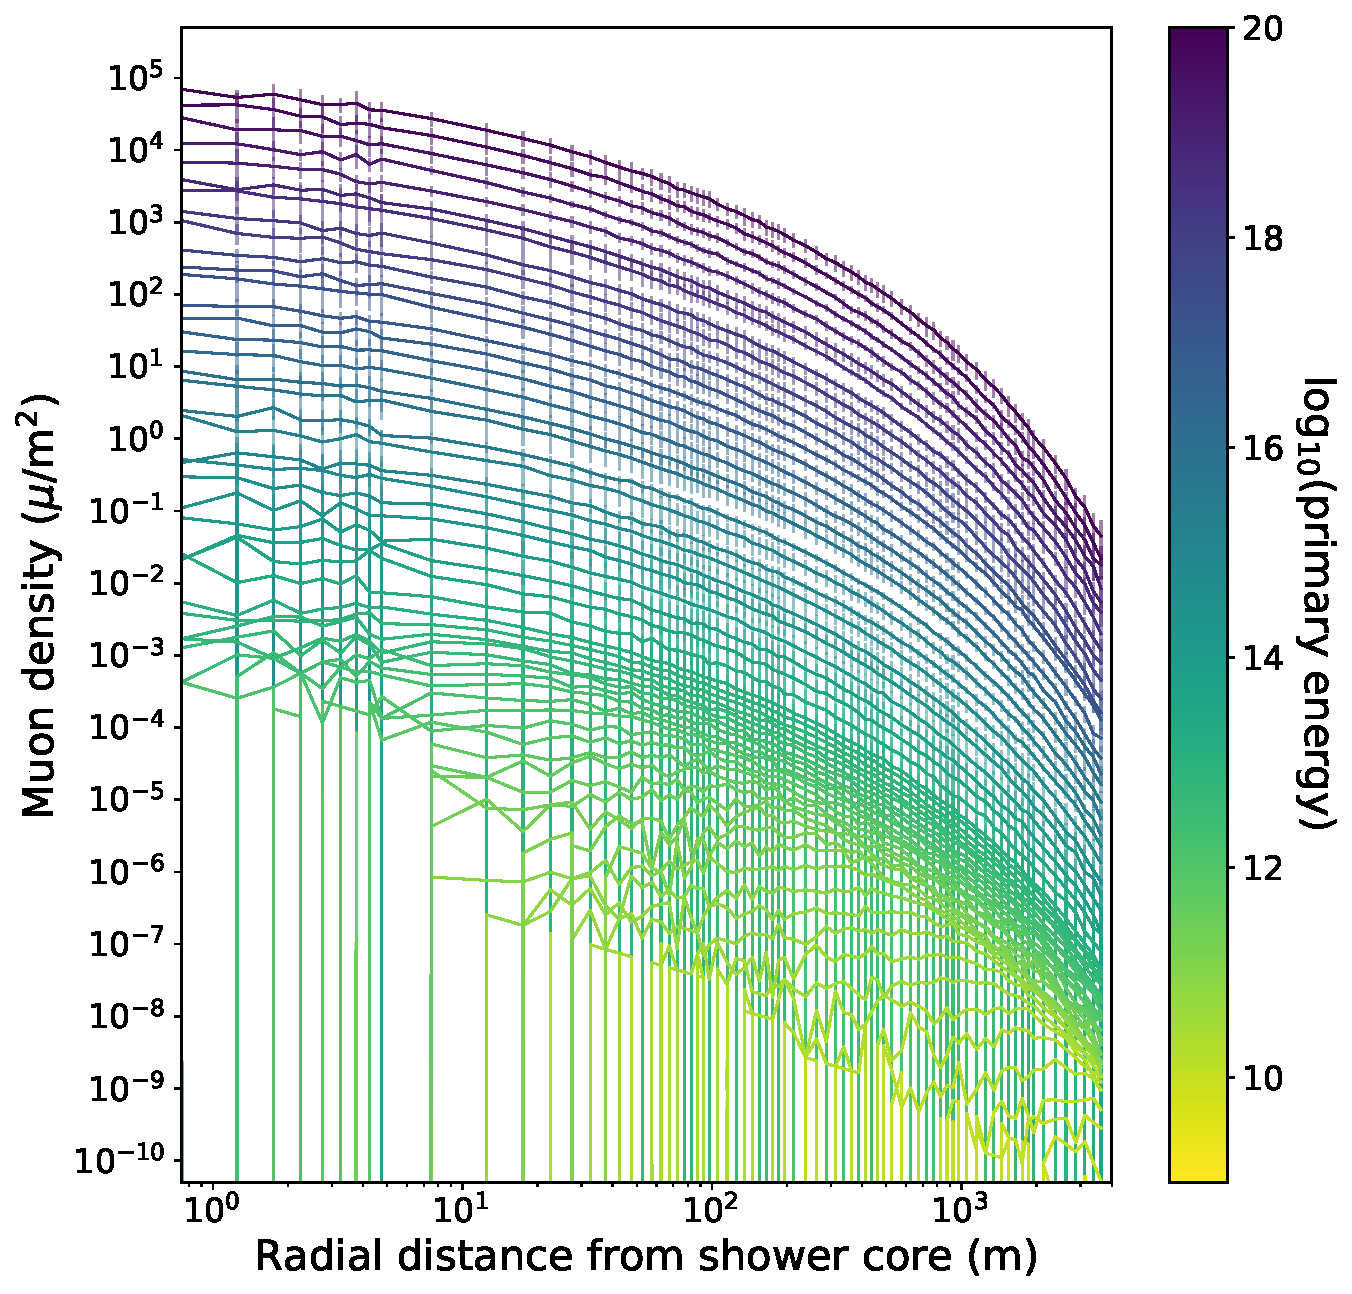
\includegraphics[width=0.47\columnwidth]{proton_footprint.pdf}} 
	\qquad
	\subfloat[$\alpha$-particle initiated air shower. \label{fig:a_footprint}]{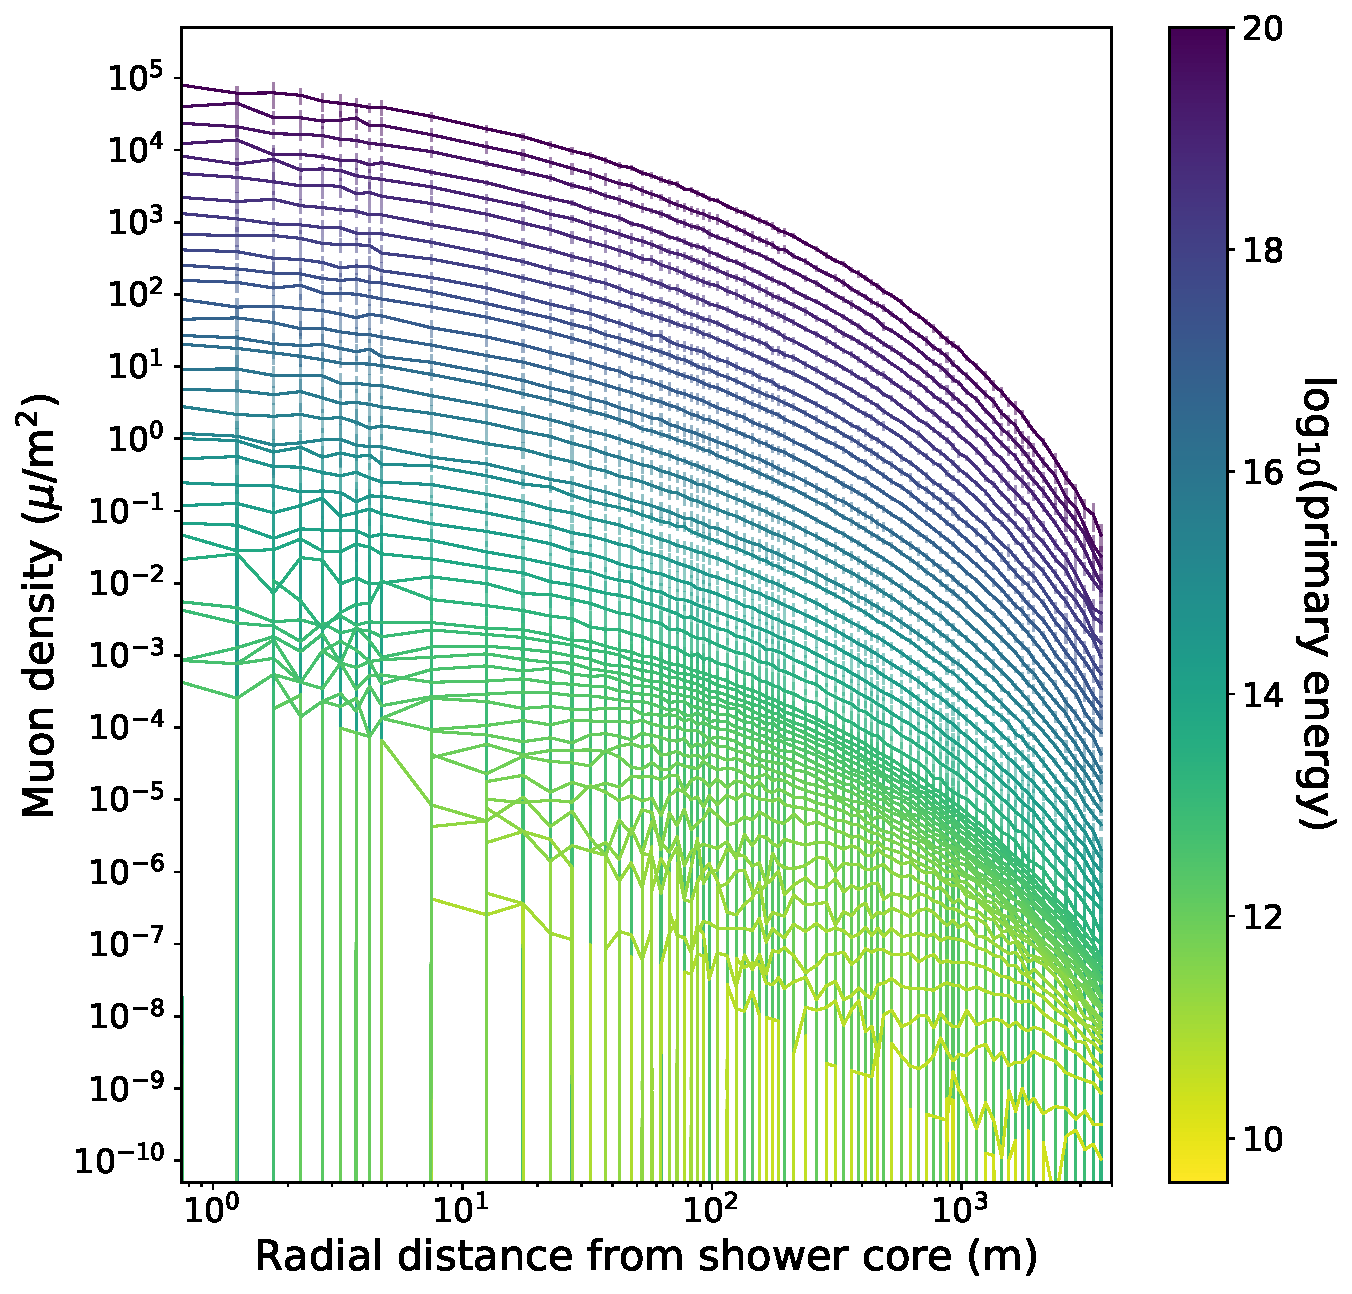
\includegraphics[width=0.47\columnwidth]{alpha_footprint.pdf}}
	\caption{Mean muon density footprints for (a) proton-initiated air showers and (b) $\alpha$-particle-initiated air showers with initial PCR trajectories with zenith angles $\theta=0^{\circ}$ and various PCR energies. The error bars given represent 1$\sigma$.} \label{fig:shower_footprints}
\end{figure}

The interpretation of Figure~\ref{fig:shower_footprints} provides an understanding of the minimum energy \glspl{pcr} observable by the different stations within the HiSPARC network. The typical separation between the detectors in a HiSPARC station is $\sim 10$~m; however, the separation between detectors varies from station-to-station and can be up to as much as some 20~m or as low as just a couple of metres. From the simulations we inferred that the variation in \gls{pcr} energy sampled varies marginally over this range of detector separations and suggests that HiSPARC stations will typically observe \glspl{pcr} with an energy on the order of $\sim 10^{14}-10^{15}$~eV and above, as they produce a sufficient density of muons to meet the required trigger conditions. 

This helps explain why the \glspl{gle} and \glspl{fd} were not observed in the HiSPARC events data. The effects of \glspl{gle} and \glspl{fd} are more prominent at lower \gls{pcr} rigidities and the air showers induced by the lower rigidity \gls{pcr} are not sufficient to induce an air shower that will trigger multiple detectors in a station. It was more likely that we may have observed the \glspl{gle} or \glspl{fd} in the singles data, as this only records the count rate of an individual detector, but again they were not observed, which may be explained looking at the flux of the muons at ground level.

%\begin{table}
%	\begin{center}
%		\caption{HS station minimum observable PCR energy}
%		\label{tab:footprints}
%		\begin{tabular}{l c c c}
%		\hline
%		{Station ID} & {Average separation (m)} & {Proton E$_{\mathrm{min}}$} & {$\alpha$-particle E$_{\mathrm{min}}$} \\
%		\hline
%		{501} & {11.2} & {} & {} \\
%		{14001} & {9.1} & {} & {} \\
%		{} & {} & {} & {} \\
%		\hline
%\end{tabular}
%\end{center}
%\end{table}


\subsection{Muon Flux}\label{sec:CORSIKA_flux}

From the air shower simulations it was also possible to gain an estimate of how many muons are produced per \gls{pcr}. Figure~\ref{fig:shower_muons} shows the energy distribution of muons produced per primary \gls{pcr}, for air showers induced by vertically incident protons and $\alpha$-particles.

\begin{figure}[ht!]
	\centering
	\subfloat[Proton initiated air shower. \label{fig:p_muons}]{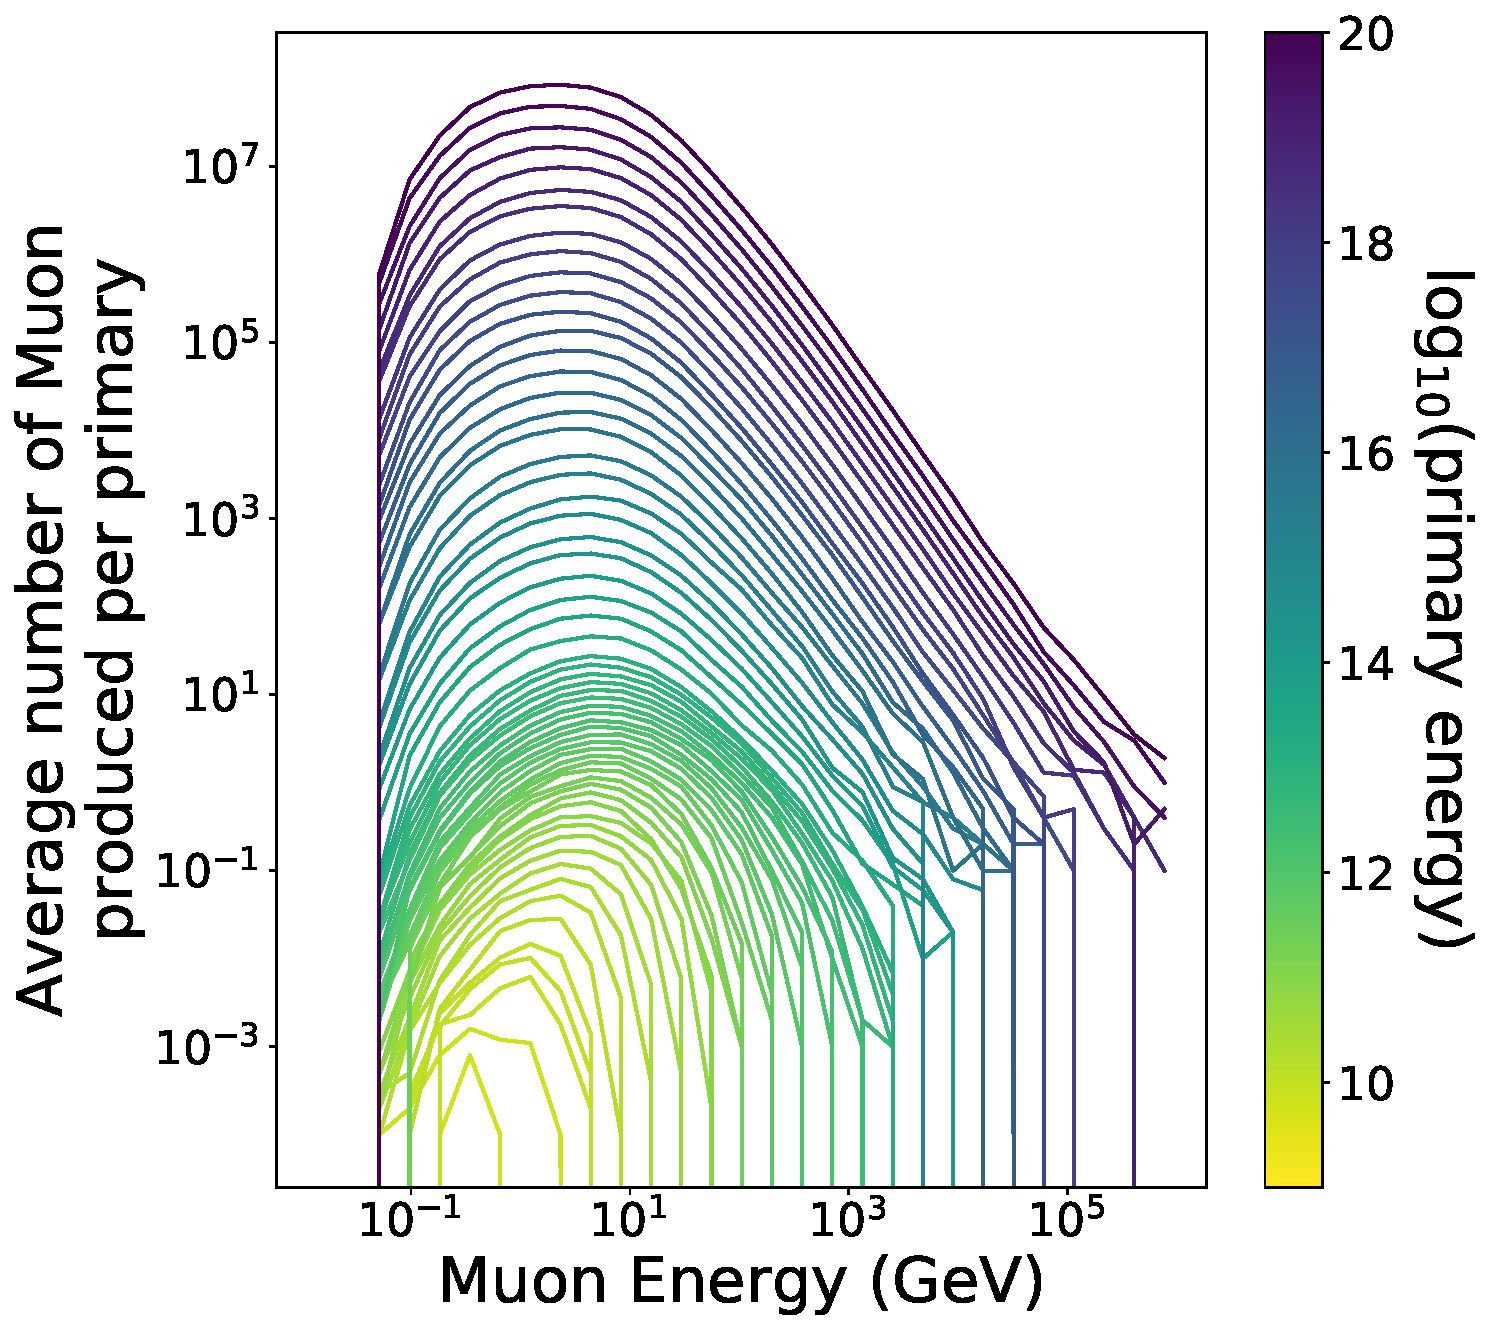
\includegraphics[width=0.47\columnwidth]{proton_muon_number.pdf}} 
	\qquad
	\subfloat[$\alpha$-particle initiated air shower. \label{fig:a_muons}]{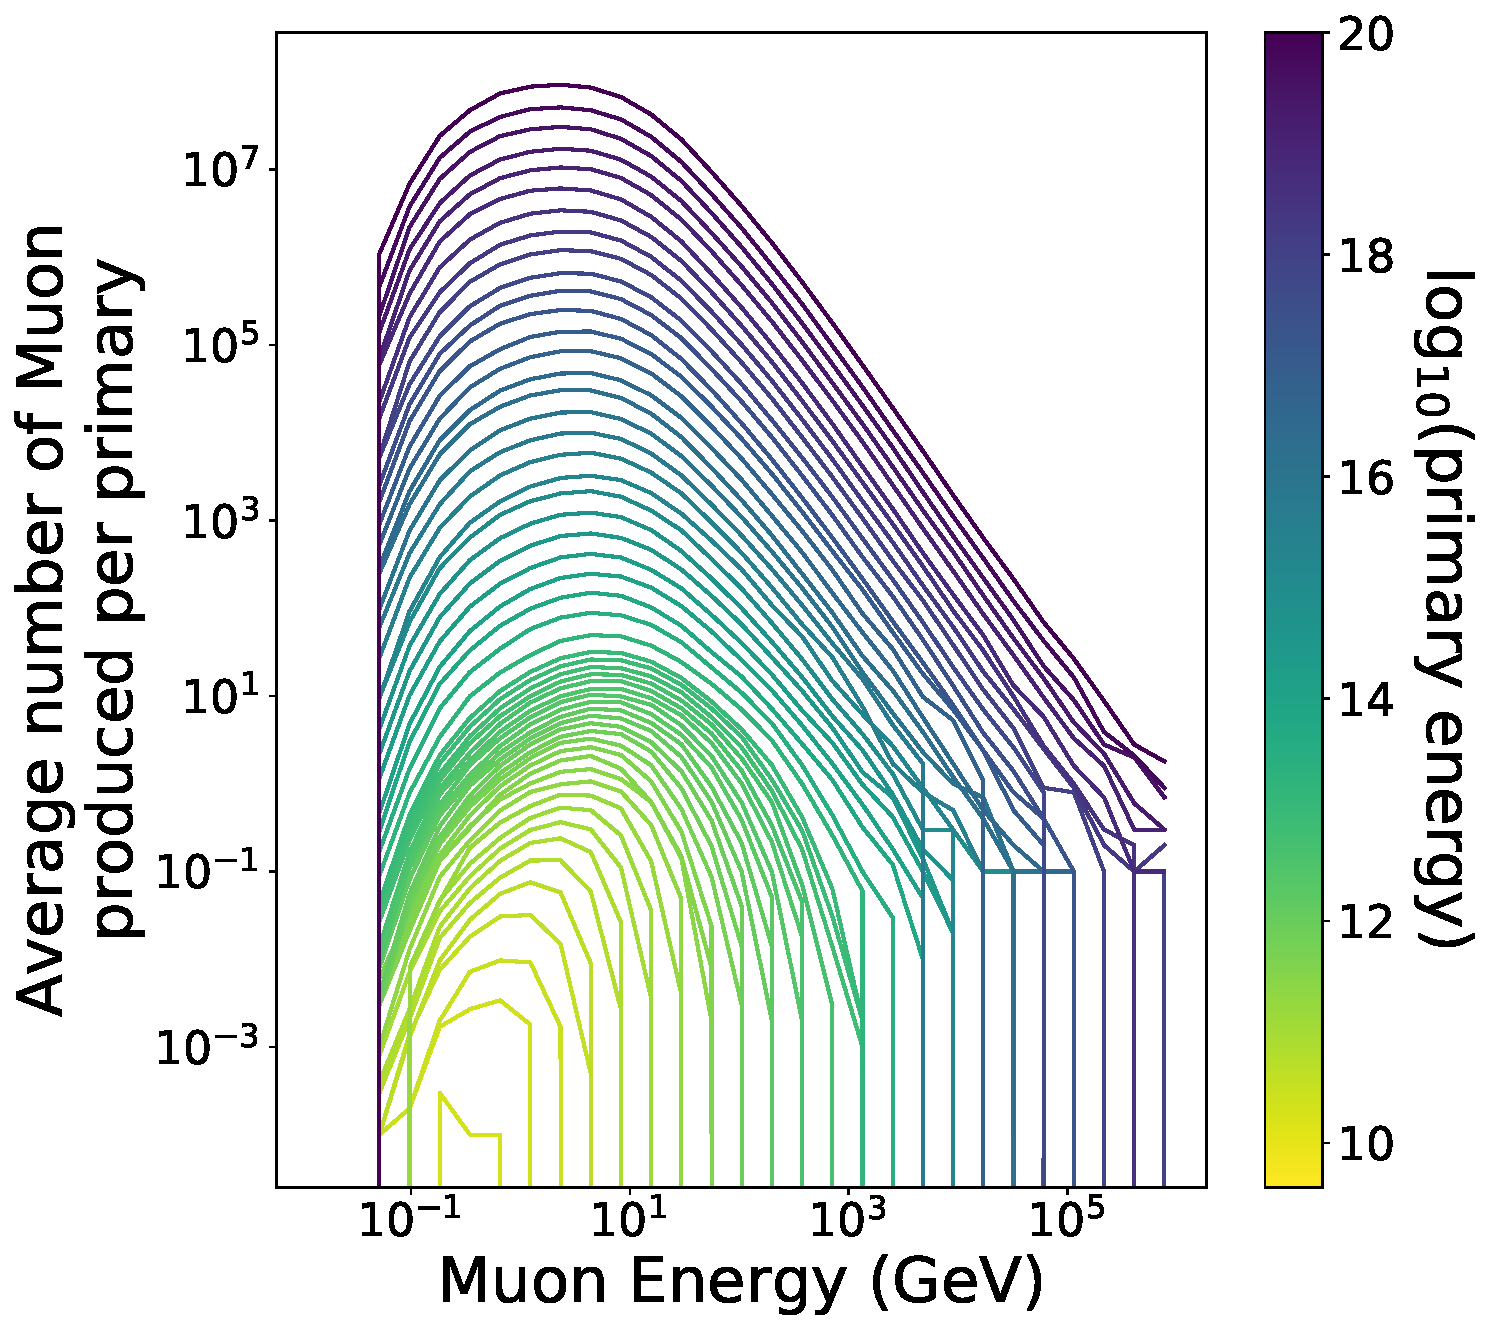
\includegraphics[width=0.47\columnwidth]{alpha_muon_number.pdf}}
	\caption{Mean number of muons produced at ground level by the PCR for (a) proton-initiated air showers and (b) $\alpha$-particle-initiated air showers, for various PCR energy.}
	\label{fig:shower_muons}
\end{figure}

The vertically incident air showers provides an upper boundary on the muon flux, but we also repeated the simulations for air showers randomly selected from a uniform distribution of incident angles between 0$^\circ$ (vertical) and 70$^\circ$, to provide a more representative flux. Similar plots were produced to those in Figure~\ref{fig:shower_muons}, but they are not shown here, as the difference is not drastically different by-eye. We see from this analysis that \glspl{pcr} with an energy less than $\sim 10^{11}-10^{12}$~eV produce only one or two muons that reach ground level, and below this \glspl{pcr} energy, it is rare that any muons are produced.

This helps explain why the \glspl{gle} and \glspl{fd} were not observed in the HiSPARC events data. The effects of \glspl{gle} and \glspl{fd} are more prominent at lower \gls{pcr} rigidities, i.e. energies <$10^9$~eV. The air showers induced by the lower rigidity \glspl{pcr} are not sufficient to produce significant increases in the flux of the muons at ground level.

We also used the data from the simulations to estimate the total muon flux at ground level, based on the \gls{pcr} flux at the top of the atmosphere. We used a model for the \gls{cr} flux, taken from \citet{corti_numerical_2019}, which utilised measurements from the \gls{ams} on-board the \gls{iss}. Figure~\ref{fig:CORSIKA_muon_spectra} shows the computed differential flux of muons at ground level, based on the simulations of vertically incident \glspl{pcr} and those randomly simulated within a 70$^\circ$ acceptance cone.

% (do this by integrating under curve, using 70-degre half-angle cone for solid angle, and area of 0.5m2)
% i.e. in python doing doing:
% where df contains the alpha and proton diff fluxes
% v = scipy.integrate.simps(df_a_v[1]+df_p_v[1], df_a_v.index.values)
% sr = 4*np.pi*(np.sin(np.deg2rad(70/2)))**2
% area = 0.5
% rate_v = v*sr*area

%\begin{figure}[ht!]
%	\centering
%	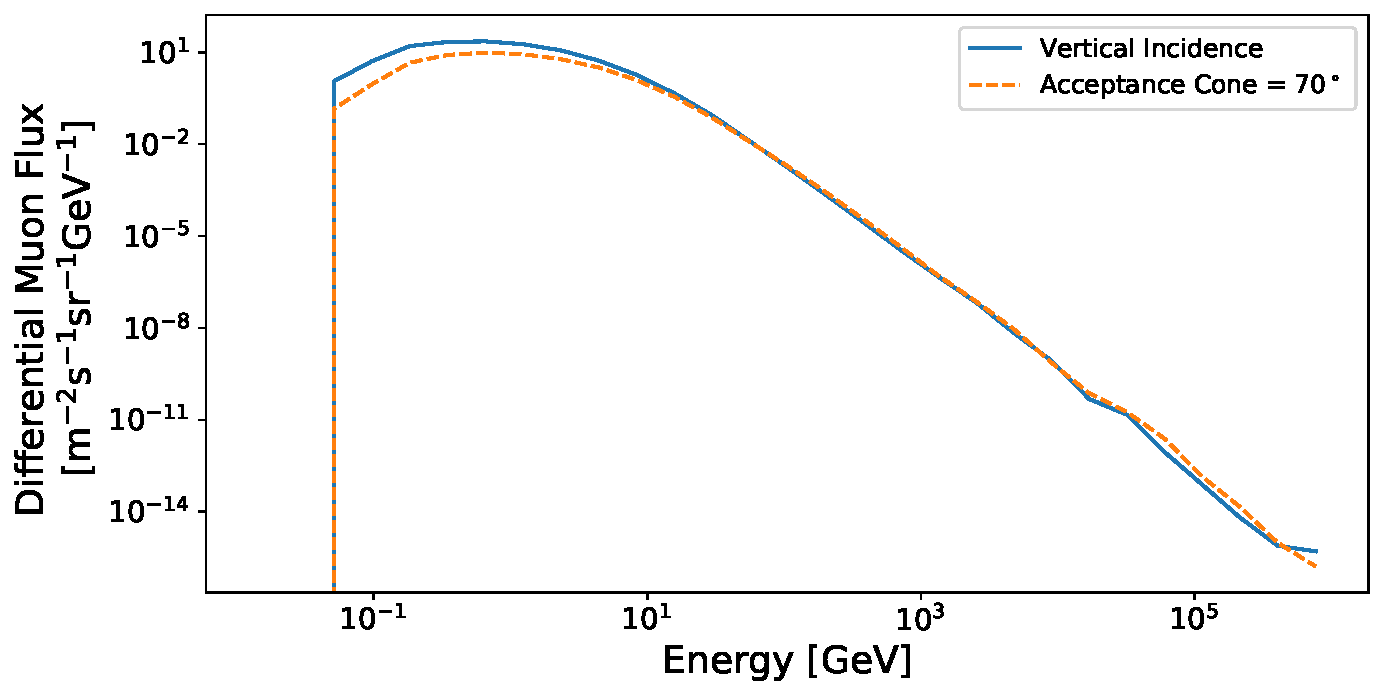
\includegraphics[width=\columnwidth]{CORSIKA_Muon_Diff_Flux_Comparison.pdf}
%	\caption{Muon differential flux computed using CORSIKA for vertically incident PCRs (solid, blue line) and for PCRs incident within an acceptance cone of $70^\circ$ (dashed, orange line).}
%	\label{fig:CORSIKA_muon_spectra}
%\end{figure}
\begin{figure}[ht!]
	\centering
	\subfloat[...]{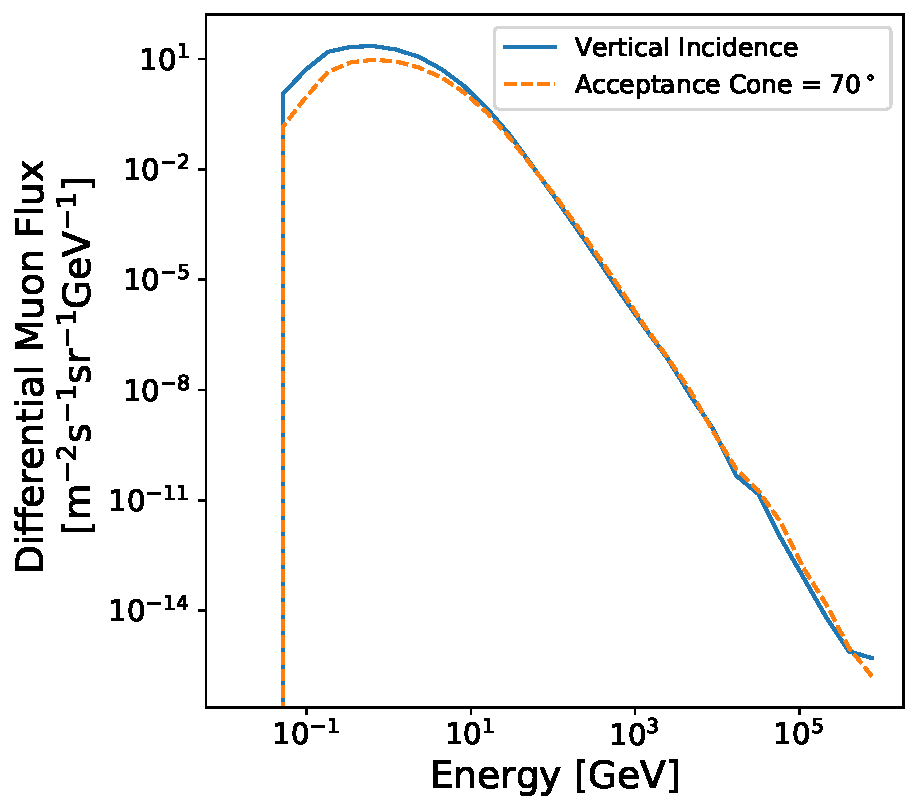
\includegraphics[width=0.47\columnwidth]{Total_Muon_Diff_Flux_Comparison.pdf}} 
	\qquad
	\subfloat[...]{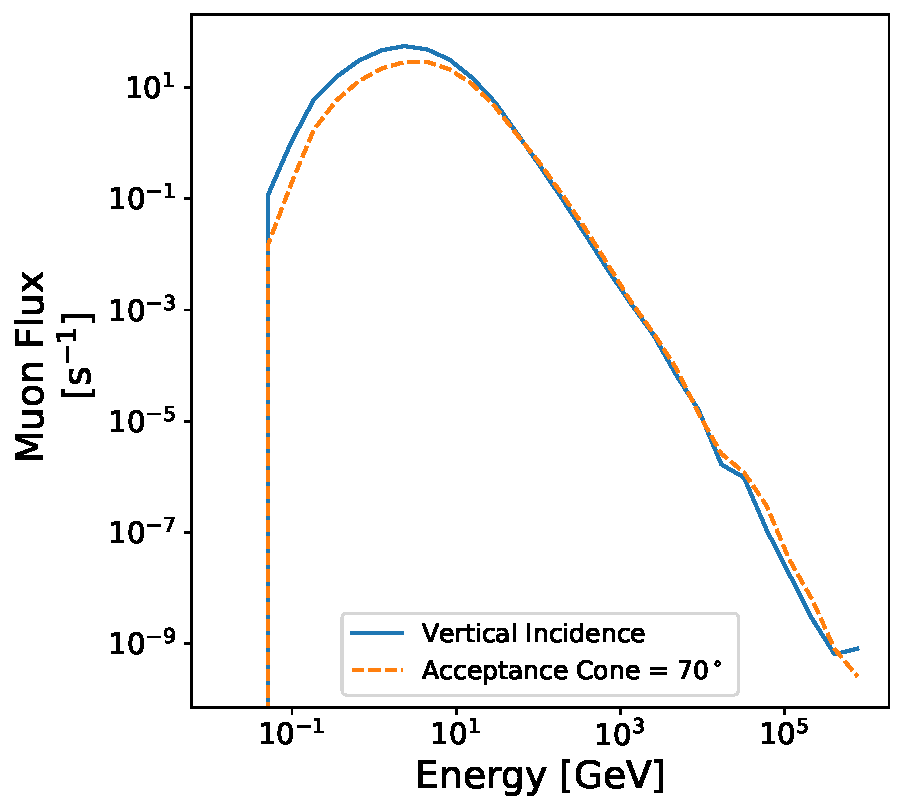
\includegraphics[width=0.47\columnwidth]{Total_Muon_Flux_Comparison.pdf}}
	\caption{...}
	\label{fig:CORSIKA_muon_spectra}
\end{figure}


From Figure~\ref{fig:CORSIKA_muon_spectra}, we see that the ground-based flux is similar for both types of simulation performed. In both, the low-energy muon flux dominates, and peak at a muon energy of $\sim 1$~GeV.

Finally, we used these calculated spectra to determine the expected rate of muons passing through a single HiSPARC detector. We computed the rates as: $85.365 \, \mu/\mathrm{s}$ (for non-vertical, i.e. $70^\circ$ acceptance cone simulations), and $156.924 \, \mu/\mathrm{s}$ (for vertical simulations). These rates are comparable to the generally accepted, average ground level muon flux of $\sim 1$ per cm$^2$ per second [cite to Autran: (https://doi.org/10.1016/j.nima.2018.06.038)].




\subsection{Muon Flux From MAIRE}\label{sec:MAIRE_flux}

As a further comparison, we used the online \gls{maire} tool to compute the muon spectrum in the atmosphere. \gls{maire} allows the computation of the secondary particle spectra in the atmosphere, caused by \glspl{sep}. \gls{maire} has a the advantage of also having the \gls{pcr} spectra for a number of \glspl{gle} built in, and therefore we obtained the muon spectra from these a few of the strongest \glspl{gle} at the Nikhef HiSPARC station (501). Figure~\ref{fig:MAIRE_muon_spectra} shows the muon spectra for a `typical' \gls{gcr} spectrum, and the additional muon spectrum for seven of the largest \glspl{gle} to date (which is additive to the \gls{gcr} spectrum).


%\begin{figure}[ht!]
%	\centering
%	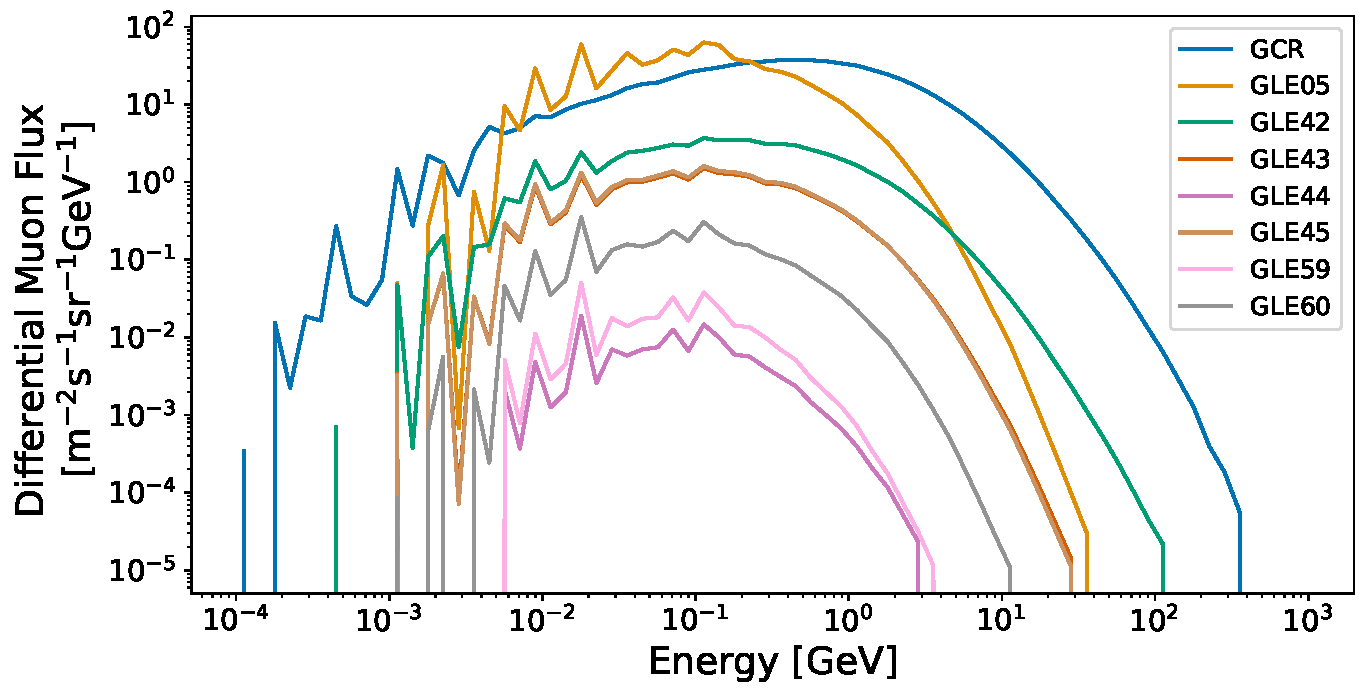
\includegraphics[width=\columnwidth]{MAIRE_Muon_Diff_Flux.pdf}
%	\caption{Muon spectrum for the typical GCR flux and during GLEs, calculated using the MAIRE tool.}
%	\label{fig:MAIRE_muon_spectra}
%\end{figure}


\begin{figure}[ht!]
	\centering
	\subfloat[...]{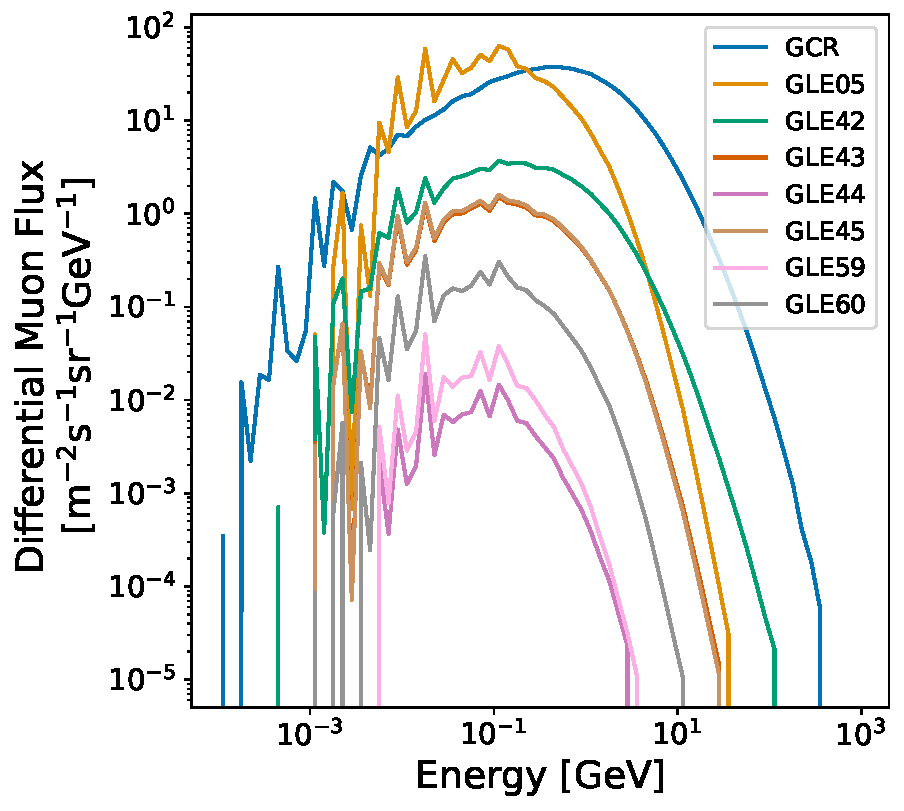
\includegraphics[width=0.47\columnwidth]{Muon_Diff_Flux.pdf}} 
	\qquad
	\subfloat[...]{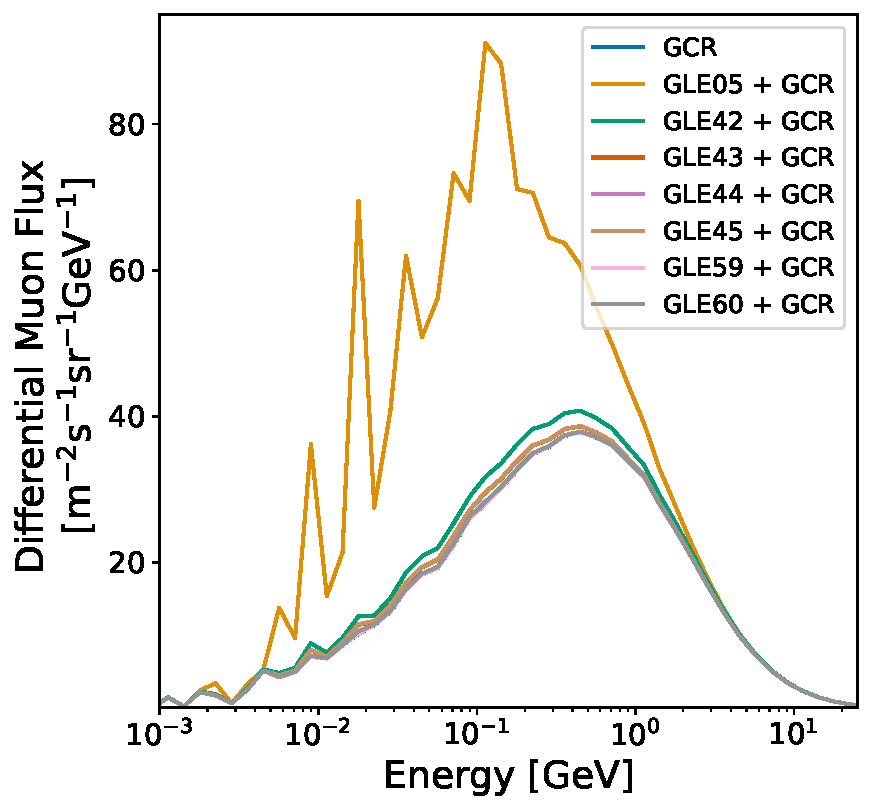
\includegraphics[width=0.47\columnwidth]{Muon_Diff_Flux_Additive.pdf}}
	\caption{...}
	\label{fig:MAIRE_muon_spectra}
\end{figure}



We can see that the \gls{gcr}-induced muon spectrum in Figure~\ref{fig:MAIRE_muon_spectra} roughly agrees with that computed using \gls{corsika}, which provides confidence in the results of both simulations. We can see that the effect on the muon spectrum drastically varies for the seven \glspl{gle}. The increase in the muon count rate was calculated based on the integrated flux compared to the background, \gls{gcr} flux, and these are also shown in Table~\ref{tab:MAIRE_GLEs}. To provide a good comparison, the approximate, maximum increase in the \gls{nm} count rate for each of the \glspl{gle} is also summarised in Table~\ref{tab:MAIRE_GLEs}. 


\begin{table}
	\begin{center}
		\caption{The increase in the predicted muon flux through a HiSPARC detector and measured neutron monitor count rate compared to the background GCR flux for the seven GLEs whereby the MAIRE muon spectra was available.}
		\label{tab:MAIRE_GLEs}
		\begin{tabular}{l c c c c c}
			\hline
			 &  & \multicolumn{2}{c}{\bf \% Change} \\
			{\bf GLE} & {\bf Date} & {\bf MAIRE muon rate} & {\bf NM station} \\
			\hline
			5 & 23/02/1956 & 20\% & $\sim 5100\%$ (Leeds) \\
			42 & 29/09/1989 & 4\% & $\sim 240 \pm 40\%$ (McMurdo) \\
			43 & 19/10/1989 & 0.8\% & $\sim 40 \pm 2\%$ (McMurdo) \\
			44  & 22/10/1989 & 0.002\% & $\sim 190 \pm 5\%$ (McMurdo) \\
			45  & 24/10/1989 & 0.8\% & $\sim 110 \pm 5\%$ (McMurdo) \\
			59 & 14/07/2000 & 0.005\% & $\sim 30 \pm 5\%$ (McMurdo) \\
			60 & 15/04/2001 & 0.07\% & $\sim 90 \pm 10\%$ (McMurdo) \\
			\hline
		\end{tabular}
	\end{center}
\end{table}
%5 & 23/02/1956 & 20\% & $\sim 5100\%$ (Leeds) \\
%42 & 29/29/1989 & 4\% & $\sim 340\%$ (Calgary) \\
%43 & 19/10/1989 & 0.8\% & $\sim 90\%$ (South Pole) \\
%44  & 22/10/1989 & 0.002\% & $\sim 190\%$ (McMurdo) \\
%45  & 24/10/1989 & 0.8\% & $\sim 200\%$ (South Pole) \\
%59 & 14/07/2000 & 0.005\% & $\sim 60\%$ (South Pole) \\
%60 & 15/04/2001 & 0.07\% & $\sim 220\%$ (South Pole) \\

The effects of these \glspl{gle} are all very large, and the only modern \gls{gle} (i.e. in Table~\ref{tab:space_weather_events}) that is comparable to any of these is \gls{gle} 70, which is comparable to \gls{gle} 43 and 59. Unfortunately, there are few HiSPARC observations due to the immaturity of the project at the time and we have shown that we do not observe \gls{gle} 70 in the HiSPARC data.

The additional contribution from the \glspl{gle} is small, and for most of the \glspl{gle}, only contributes an increase of $\sim 10 \%$ in the ground-level muon flux. The exception in Figure~\ref{fig:MAIRE_muon_spectra} is for \gls{gle} 5, but this was an exceptionally large event, for which we haven't seen anything similar in over half a decade; such events are rare. We expect that we would have seen this increase in the HiSPARC data, but, of course, this event pre-dated the HiSPARC project.

These simulations, combined with the figures detailed in Table~\ref{tab:space_weather_events} and Table~\ref{tab:MAIRE_GLEs}, show us that we would have expected an increase in the muon spectrum of no more than $\sim 1\%$ (and more likely on the order of $\sim 0.1\%$) for both \gls{gle} 71 and 72, which rules their observation with HiSPARC as extremely unlikely.




%%%%%%%%%%%%%%%%%%%%%%%%%%%%%%%%%%%%%%%%%%%%%%%%%%%%%%%%%%%%%%%%%%%%%
%%%%%%%%%%%%%%%%%%%%%%%%%%%%%%%%%%%%%%%%%%%%%%%%%%%%%%%%%%%%%%%%%%%%%
\section{Standardisation of HiSPARC Data}\label{sec:HS_standardisation}

%%%%%%%%%%%%%%%%%%%%%%%%%%%%%%%%%%%%%%%%%%%%%%%%%%%%%%%%%%%%%%%%%%%%%
\subsection{Motivation}
- HiSPARC stations are individually managed and guidelines aren't stringent

- Variability between stations exists and also apparently between detectors within a station (i.e. see singles during \gls{gle} 72)

- We have seen that the stations are sensitive to their local atmospheric conditions...

%%%%%%%%%%%%%%%%%%%%%%%%%%%%%%%%%%%%%%%%%%%%%%%%%%%%%%%%%%%%%%%%%%%%%
\subsection{Barometric Correction}\label{sec:HS_P_corr}

Observations made by ground-based \gls{cr} detectors are susceptible to atmospheric conditions. Atmospheric pressure effects the \gls{cr} path length due to the expansion and contraction of the atmosphere with varying pressure; hence the \gls{cr} counts are observed to be negatively correlated to atmospheric pressure as shown for both \glspl{nm} and \glspl{md} in Figure~\ref{fig:CR_V_P}. A correction for this barometric effect is routinely applied as part of the data calibration for all \gls{nm} stations within the \gls{nmdb} NEST, but there is no such process routinely applied in the HiSPARC networks data pipeline.


\begin{figure}[ht]
	\centering
	\subfloat[NM Station]{
		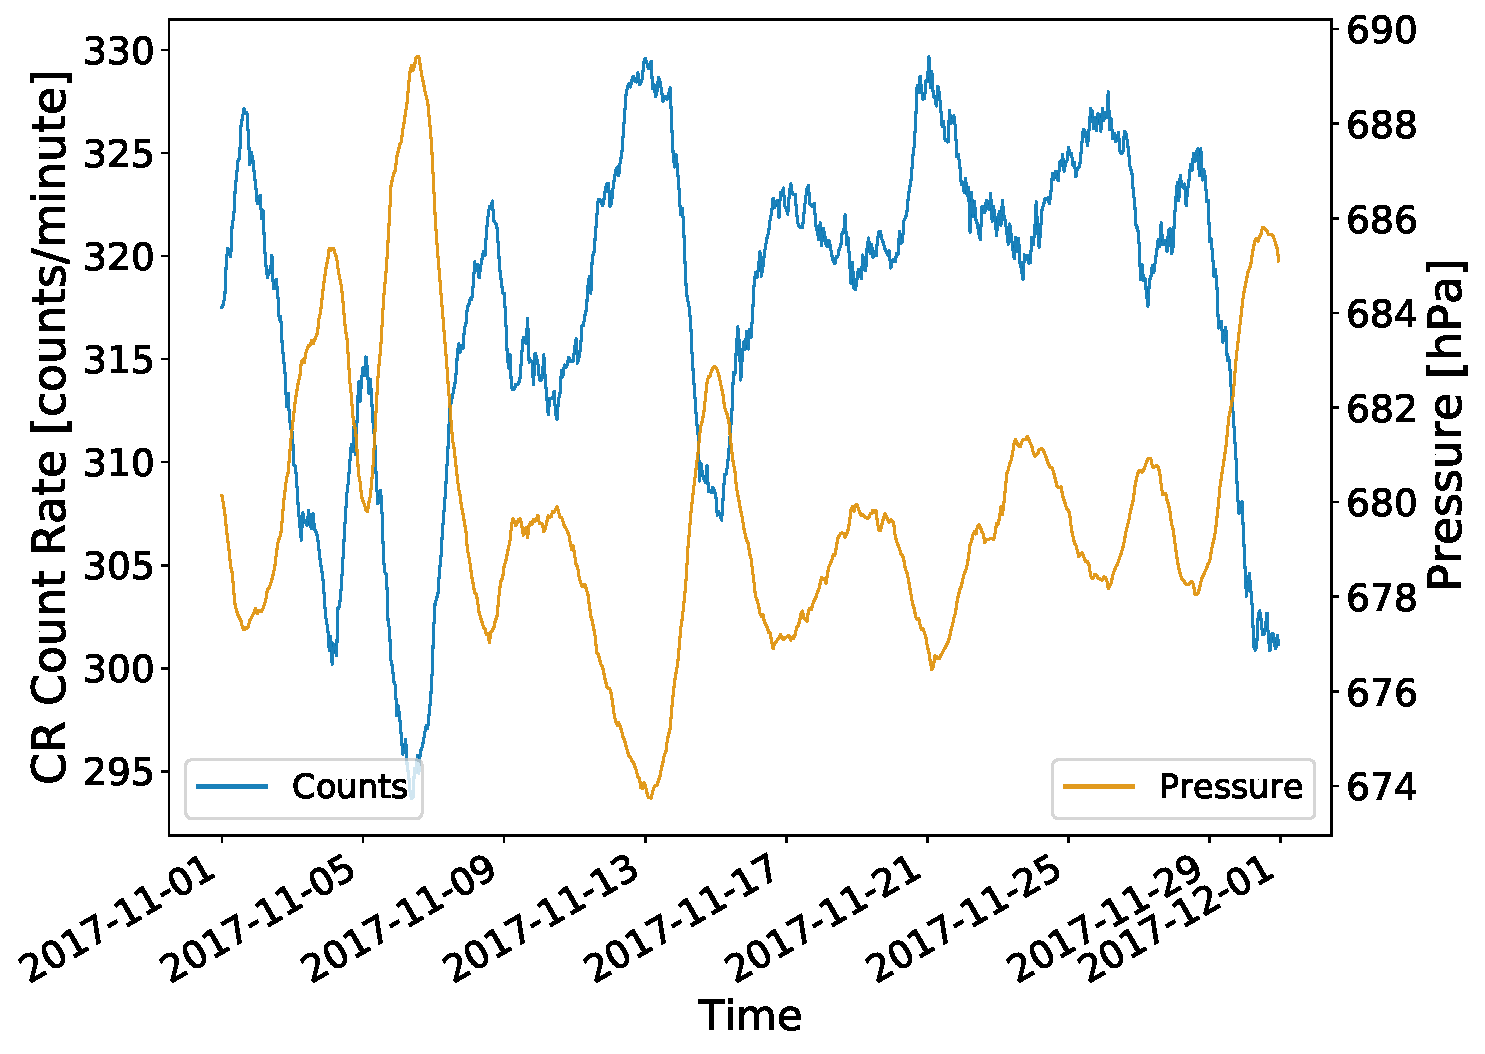
\includegraphics[width=0.48\columnwidth]{SOPO_CRvP.pdf}
		\label{fig:SOPO_CRvP}}
	%\qquad
	\subfloat[HS 501 (Nikhef)]{
		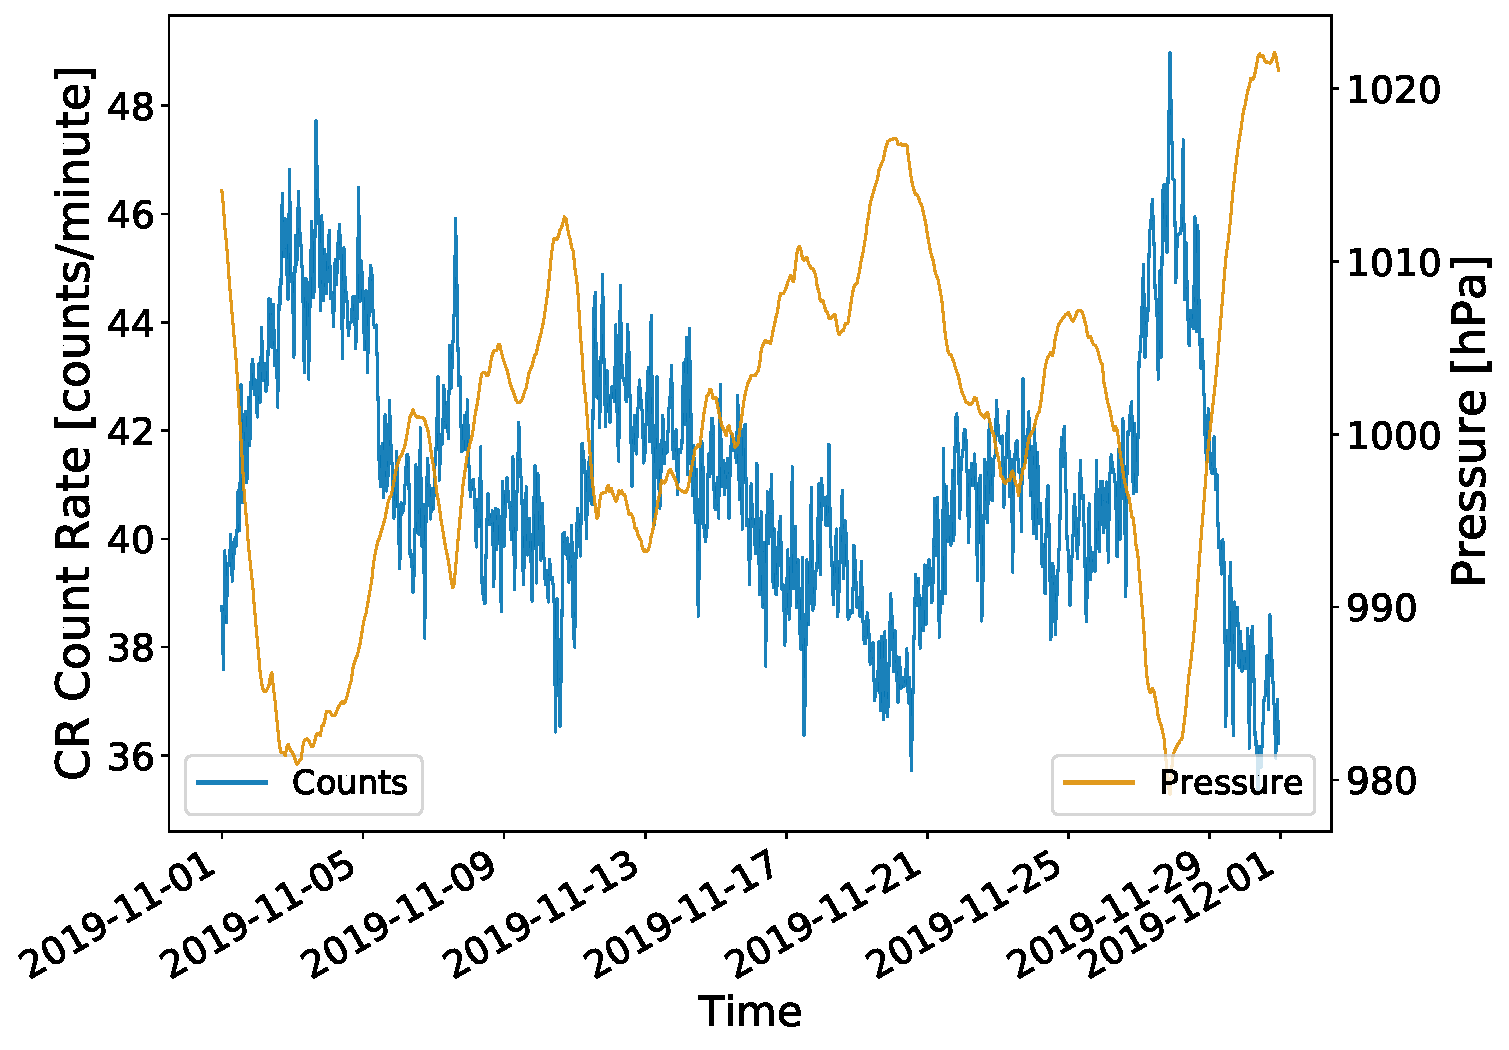
\includegraphics[width=0.48\columnwidth]{501_CRvP.pdf}
		\label{fig:HS_501_CRvP}} \\
	
	\caption{The anti-correlation between CR count rates and the atmospheric pressure. (a) shows the CR and the local atmospheric pressure measured at a NM in the South Pole; (b) shows the CR and pressure measured by HiSPARC station 501.}
	\label{fig:CR_V_P}
\end{figure}


The method of correcting for the barometric effect is discussed widely in the literature regarding \glspl{nm} and is shown to depend on the barometric coefficient. Assuming the cosmic ray flux variation, absent of the atmospheric effects, is reasonably stable, then a simple correction to the counts can be made. The \gls{cr} variations ($N$) that depend on the local atmospheric pressure are described by equation~(\ref{eq:presscorr1}), where $\Delta N$ is the change in count rate, $\beta$ is the barometric coefficient, and $\Delta P = P - P_0$ is the deviation in pressure from the average ($P_0$) in the given time-period \citep{paschalis_online_2013}:

\begin{equation}
\Delta N = - \beta \, N \, \Delta P
\label{eq:presscorr1}
\end{equation}

Through the integration of equation~(\ref{eq:presscorr1}), the solution shows the dependence of cosmic ray intensity on pressure as given in equation~(\ref{eq:presscorr2}). 

\begin{equation}
N = N_{0} \, e^{-\beta \, \Delta P}
\label{eq:presscorr2}
\end{equation}

Therefore by taking the logarithm of equation~(\ref{eq:presscorr2}), one can obtain the barometric coefficient by fitting the straight line given by equation~(\ref{eq:presscorr3}) to the observed data, where $N_0$ may be assumed as the mean count rate over the given time-period of observations considered.

\begin{equation}
\mathrm{ln} \left( \frac{N}{N_0} \right) = - \beta \, \Delta P
\label{eq:presscorr3}
\end{equation}

A demonstration of the barometric correction method of fitting a straight line to the data described by equation~(\ref{eq:presscorr3}) is shown for both a NM and a HiSPARC station in Figure~\ref{fig:barometric_fit}.

\begin{figure}[ht]
	\centering
	\subfloat[SOPO NM Station]{
		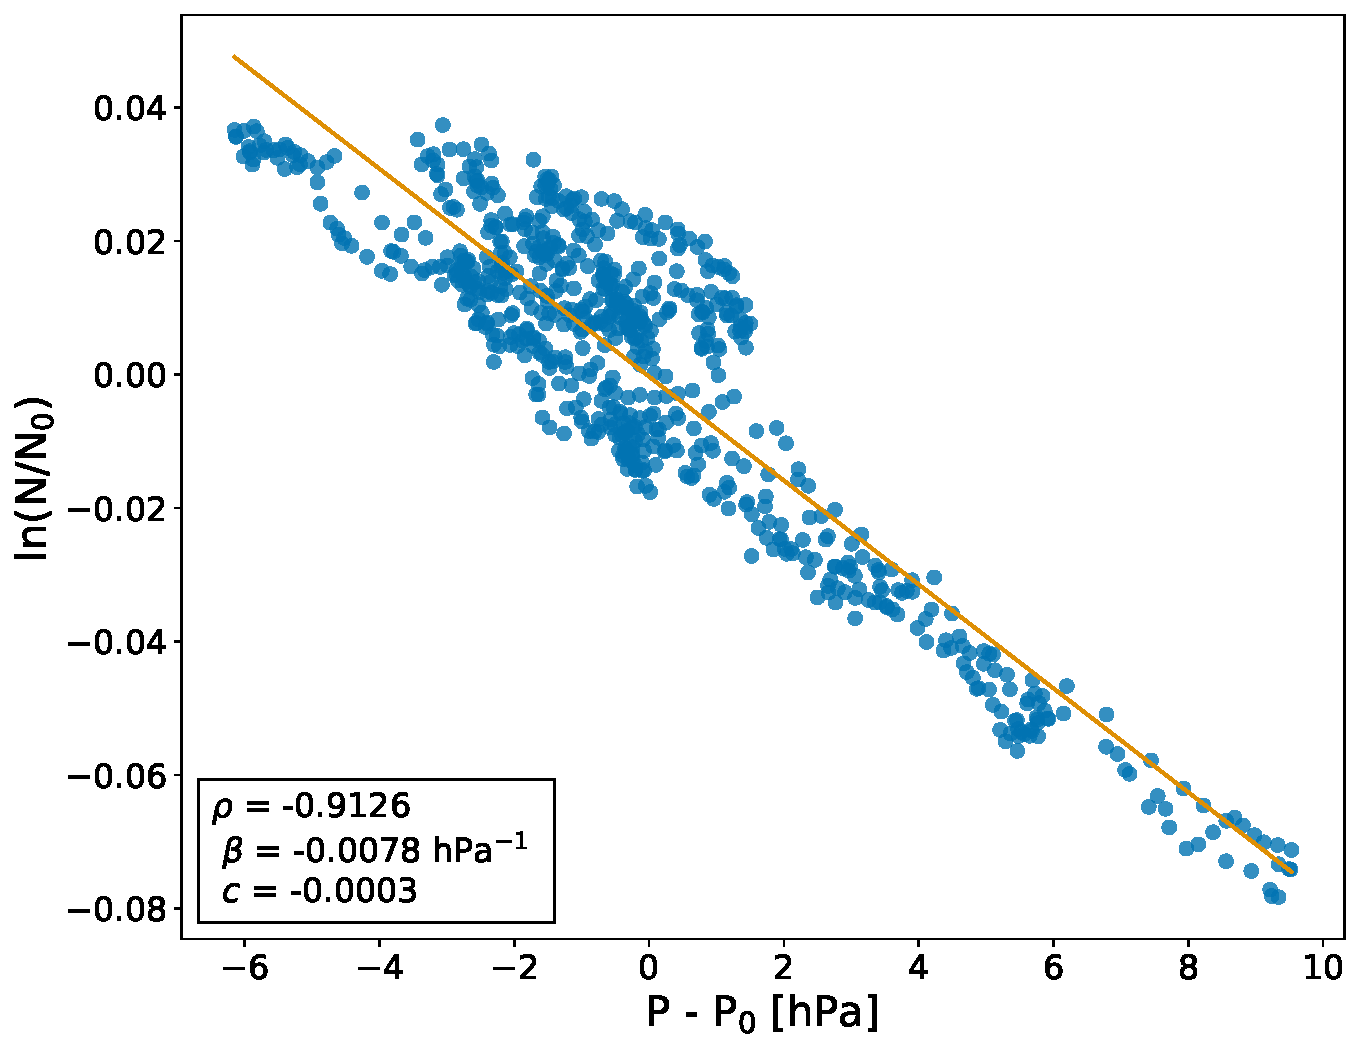
\includegraphics[width=0.48\columnwidth]{SOPO_beta.pdf}
		\label{fig:SOPO_beta}}
	%\qquad
	\subfloat[HS 501 (Nikhef)]{
		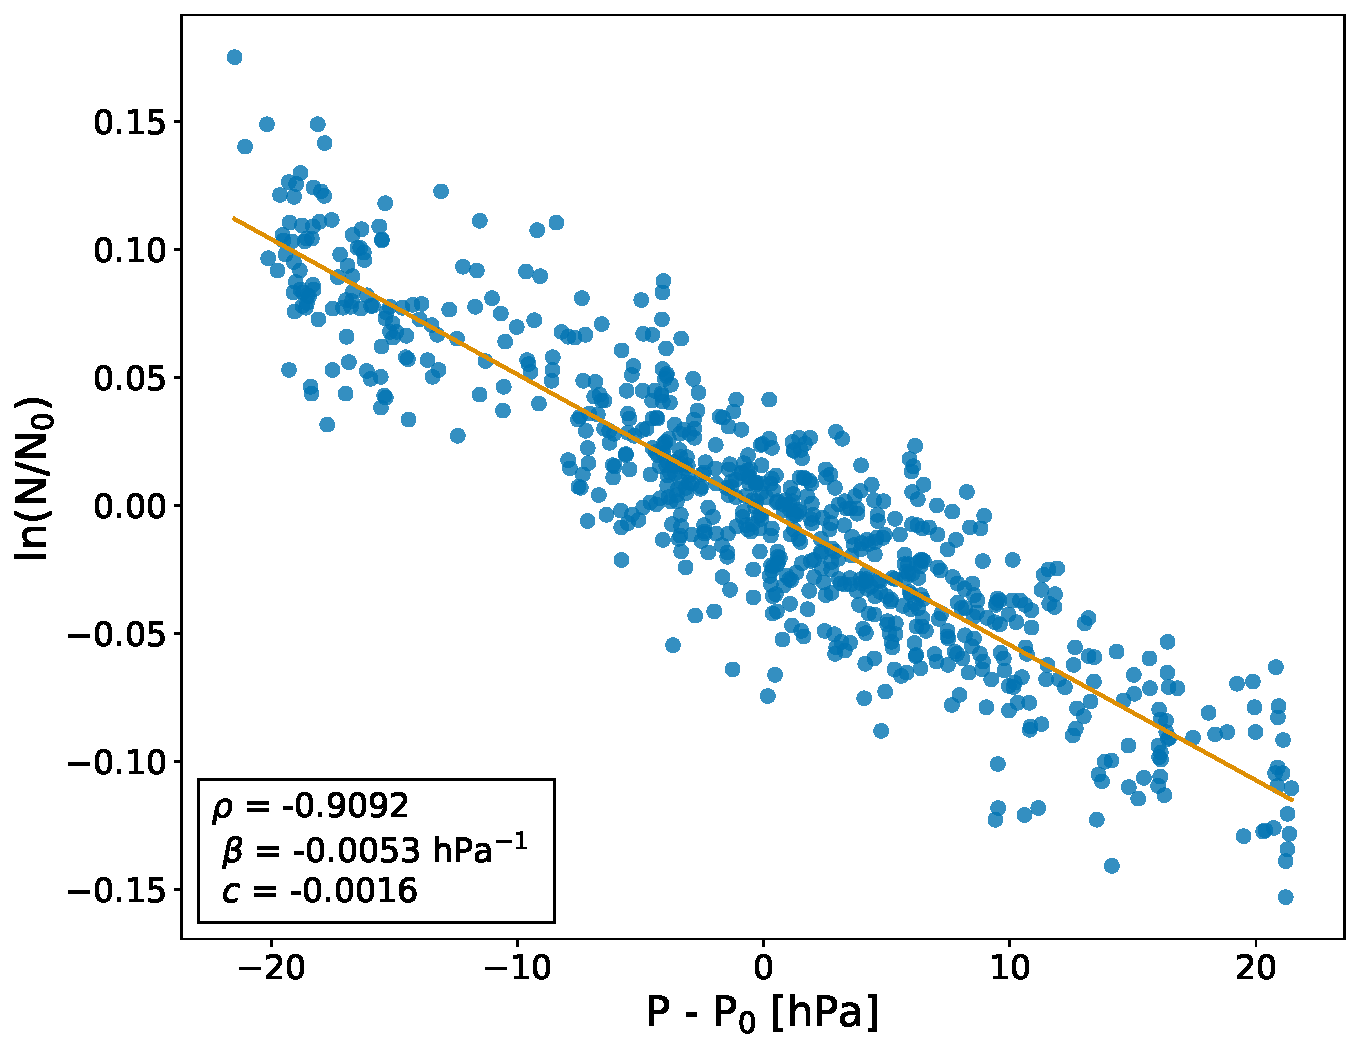
\includegraphics[width=0.48\columnwidth]{501_beta.pdf}
		\label{fig:HS_501_beta}} \\
	
	\caption{The barometric coefficient calculation: (a) during November 2017 for the South Pole (SOPO) NM station, (b) during November 2019 for HiSPARC station 501 at Nikhef.}
	\label{fig:barometric_fit}
\end{figure}


An online barometric coefficient tool\footnote{\url{http://cosray.phys.uoa.gr/index.php/data/nm-barometric-coefficient}} is available for \glspl{nm}, which allows users to perform the barometric correction for a given station over a user-defined epoch \citep{paschalis_online_2013}. Using this tool, it was possible to provide a comparison between the method used in this work to that of the online \gls{nm} barometric correction tool which is used for the correction of the \gls{nmdb} stations. This is provided in Figure~\ref{fig:NM_beta_variation} for monthly corrections throughout 2017 for the \gls{nm} station at the South Pole (SOPO).

\begin{figure}[ht]
	\centering
	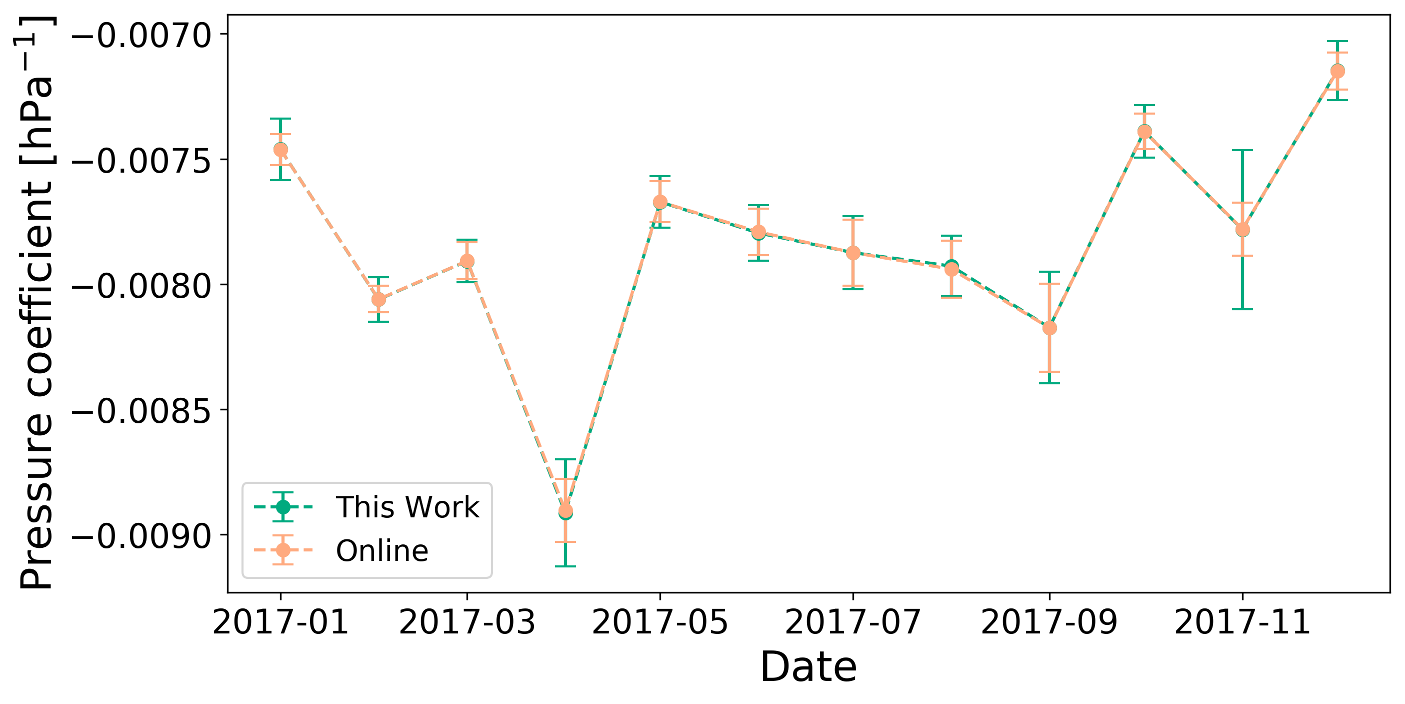
\includegraphics[width=0.65\columnwidth]{SOPO_beta_2017_rescale.png}
	\caption{A comparison between the monthly barometric coefficient computed in this work and using the online barometric coefficient tool throughout the year 2017 for the SOPO NM station.}
	\label{fig:NM_beta_variation}
\end{figure}


Figure~\ref{fig:NM_beta_variation} shows a close agreement between the barometric coefficient calculated in this work and those acquired from the online tool for the SOPO \gls{nm}. This was also true for other stations tested (APTY and ROME), thus providing confidence that the method used in this work was suitable for application on the HiSPARC data. The barometric correction was performed on the stations where sufficient pressure data and count rates exist, and were re-investigated to determine whether the space weather events were observed in the HiSPARC data. These results are provided in Section \ref{sec:HS_obs_Pcorr}.

[include a time series for the variation in the barometric coefficient for HiSPARC (i.e. for station 501)...]



%%%%%%%%%%%%%%%%%%%%%%%%%%%%%%%%%%%%%%%%%%%%%%%%%%%%%%%%%%%%%%%%%%%%%
\subsection{Temperature Correction}\label{sec:HS_T_corr}

It has been discussed in the literature that the effect of atmospheric temperature on muon intensity has to be treated differently to the pressure effect \citep{berkova_temperature_2011}, as the temperature influences both the creation and disintegration processes for muons, such that there is a positive effect and a negative effect on muon intensity as a consequence of temperature variations \citep{mendoncca_temperature_2016}. 

The positive effect is related to pion decay and its dependence on temperature variation. The higher the temperature, the lower the atmospheric pion absorption, which implies a higher generation rate of muons \citep{mendoncca_temperature_2016}.

The negative effect corresponds to the decrease of muon intensity at ground level as the muon average path length varies with temperature. Due to the heating and the expansion of the atmosphere during summer periods muons are produced higher in the atmosphere; hence the muon propagation path increases meaning more atmosphere for muons to traverse before reaching the ground, and an increased decay probability and ionisation losses \citep{savic_pressure_2015, mendoncca_temperature_2016}.

Due to the difference in decay probability, the negative effects dominate for low energy muons (i.e. those detected by ground-level MDs), and the positive effect dominates for high energy muons (i.e. those detected by underground MDs) \citep{berkova_temperature_2011}; therefore it is expected that the negative effect should dominate for the HiSPARC network. Temperature effects are also observed by NMs; however the effect is less significant than for MDs hence temperature corrections are not widely applied for NMs \citep{mendoncca_temperature_2016}.

This is in contradiction with the observations of diurnal variation with the HiSPARC detector, as one can quite clearly see that the HiSPARC stations register higher count rates during local noon.

Several methods of correcting for the negative temperature effect are summarised by \cite{berkova_temperature_2011} which utilise different measures of atmospheric temperature when performing the temperature correction. \cite{mendoncca_temperature_2016} provides a comparative summary of these methods applied to correct for atmospheric temperature variations observed by GMDN detectors. The methods discussed here however are typically applied over long timescales of years with low temporal resolution rather than to account for short timescale variations with periods of less than a day; hence these methods aren't necessarily suitable for this work.

%\cite{mendoncca_temperature_2016} concludes that correcting for temperature using the atmospheric mass weighted temperature is one of the most suitable methods for the GMDN as it allows for the highest correlation between long-term \gls{cr} variations and temperature. The mass weighted method is an approximation for integrating over the vertical atmospheric temperature as is given in Eq. (\ref{eq:tempcorr}):
%
%\begin{equation}
%\left( \frac{\Delta N}{N} \right)_T = \, \bar{\alpha}  \int^{h_0}_{0}  \, \delta \, T(h) \, dh = \sum_{i=0}^{n} \frac{x(h_i) - x(h_{i+1})}{x(h_0)} T(h_i)  = \alpha_{\mathrm{MSS}} \delta T_{\mathrm{MSS}}
%\label{eq:tempcorr}
%\end{equation}
%
%where $h_0$ is the closest to ground altitude; $\delta T_{\mathrm{MSS}}$ is the deviation of the mass weighted atmospheric temperature; $T(h_i)$ is the temperature in degrees kelvin observed at the altitude $h_i$; $x(h_ i)$ is the atmospheric depth at the altitude $h_i$ which is given by Eq. \ref{eq:atmos_depth}:
%
%\begin{equation}
%x(h) = \int^{\infty}_{h}  \, \rho (h) \, dh  \, \rho (h) = \frac{P(h)}{T(h)} \frac{M_{mol}}{R} 
%\label{eq:atmos_depth}
%\end{equation}
%
%where $P(h)$ is the atmospheric pressure profile as a function of depth; $T(h)$ is the atmospheric temperature; $\rho(h)$ is the air density at a given altitude $h$; $M_{mol}$ is the molar mass of air; $R$ is the universal gas constant.
%
%The temperature correction is therefore used in a formalism the same as Eq. (\ref{eq:presscorr3}), replacing replacing $\beta$ for $\alpha$ and $\Delta P$ for $\Delta T$.
%
%In addition it is discussed by \cite{berkova_temperature_2011} and \cite{mendoncca_temperature_2016} that the effective generation level temperature is a suitable assumption for this purpose. This method is based on the assumption that muons are mostly generated at a certain isobaric level, taken as 100 mbar, and therefore the temperature at 100 mbar in the atmospheric pressure profile is used, $T_{\mathrm{100 \, mbar}}$.
%
%As discussed above, \cite{mendoncca_temperature_2016} provide this as a method for correcting for the long-term variation in atmospheric temperature which varies seasonally rather than to correct for diurnal variations; therefore it is unsure how relevant this method of atmospheric temperature correction will be to the diurnal variations observed in the HiSPARC data.

[finally discuss, in connection with the diurnal effect, that the HiSPARC stations don't really have a suitable measure of temperature. They provide the local outdoor temperature, nearby, and also the temperature in the room where the electronics are (useless...)... so limited capacity to be able to do a good job on the temperature correction...]

 

%%%%%%%%%%%%%%%%%%%%%%%%%%%%%%%%%%%%%%%%%%%%%%%%%%%%%%%%%%%%%%%%%%%%%
%%%%%%%%%%%%%%%%%%%%%%%%%%%%%%%%%%%%%%%%%%%%%%%%%%%%%%%%%%%%%%%%%%%%%
\section{HiSPARC Observations After Pressure Corrections}\label{sec:HS_obs_Pcorr}


%%%%%%%%%%%%%%%%%%%%%%%%%%%%%%%%%%%%%%%%%%%%%%%%%%%%%%%%%%%%%%%%%%%%%
\subsection{Pressure Corrected Observations of Ground Level Enhancements}

Following the pressure correction, the search for evidence of \glspl{gle} was re-conducted, this time within the pressure corrected HiSPARC data. This could only be conducted for \gls{gle} 71 and 72, as the HiSPARC network was not collecting meteorological data during the epoch of \gls{gle} 70. Figure~\ref{fig:GLE_71_Pcorr} and Figure~\ref{fig:GLE_72_Pcorr} shows the pressure-corrected HiSPARC observations around the epochs of \gls{gle} 71 and 72, respectively.

The observations of \gls{gle} 71 show only the HiSPARC events data; however, we also show the singles rates from each of the individual detectors in a station for \gls{gle} 72.

\begin{figure}[ht]
	\centering
	\subfloat[HS 3001 (Leiden)]{
		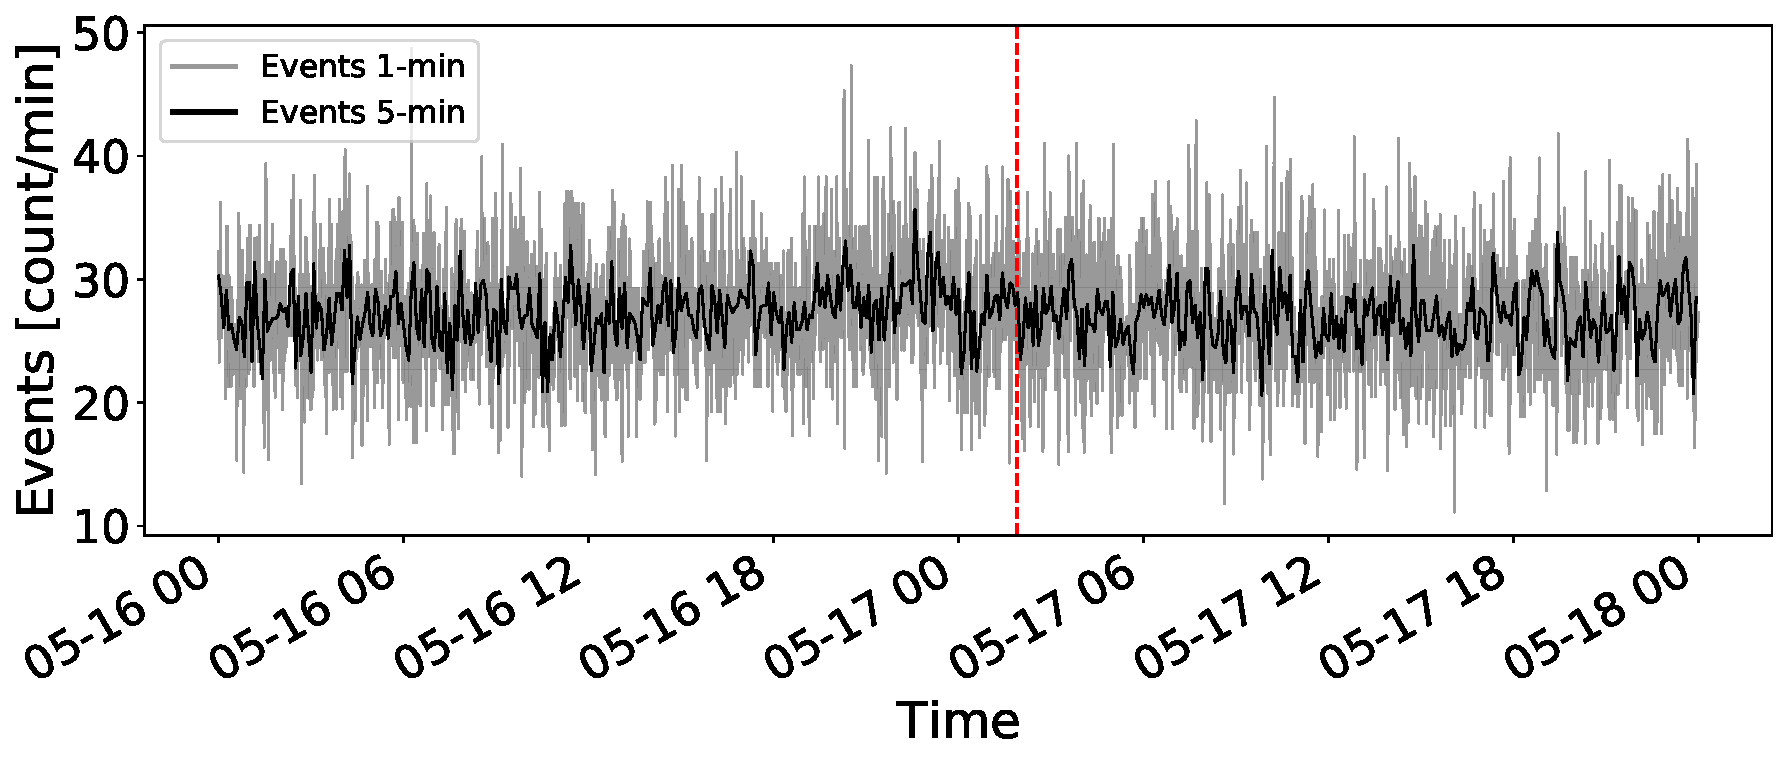
\includegraphics[width=0.48\columnwidth]{GLE71_3001_Pcorr.pdf}
		\label{fig:GLE71_3001_Pcorr}}
	%\qquad
	\subfloat[HS 8001 (Eindhoven)]{
		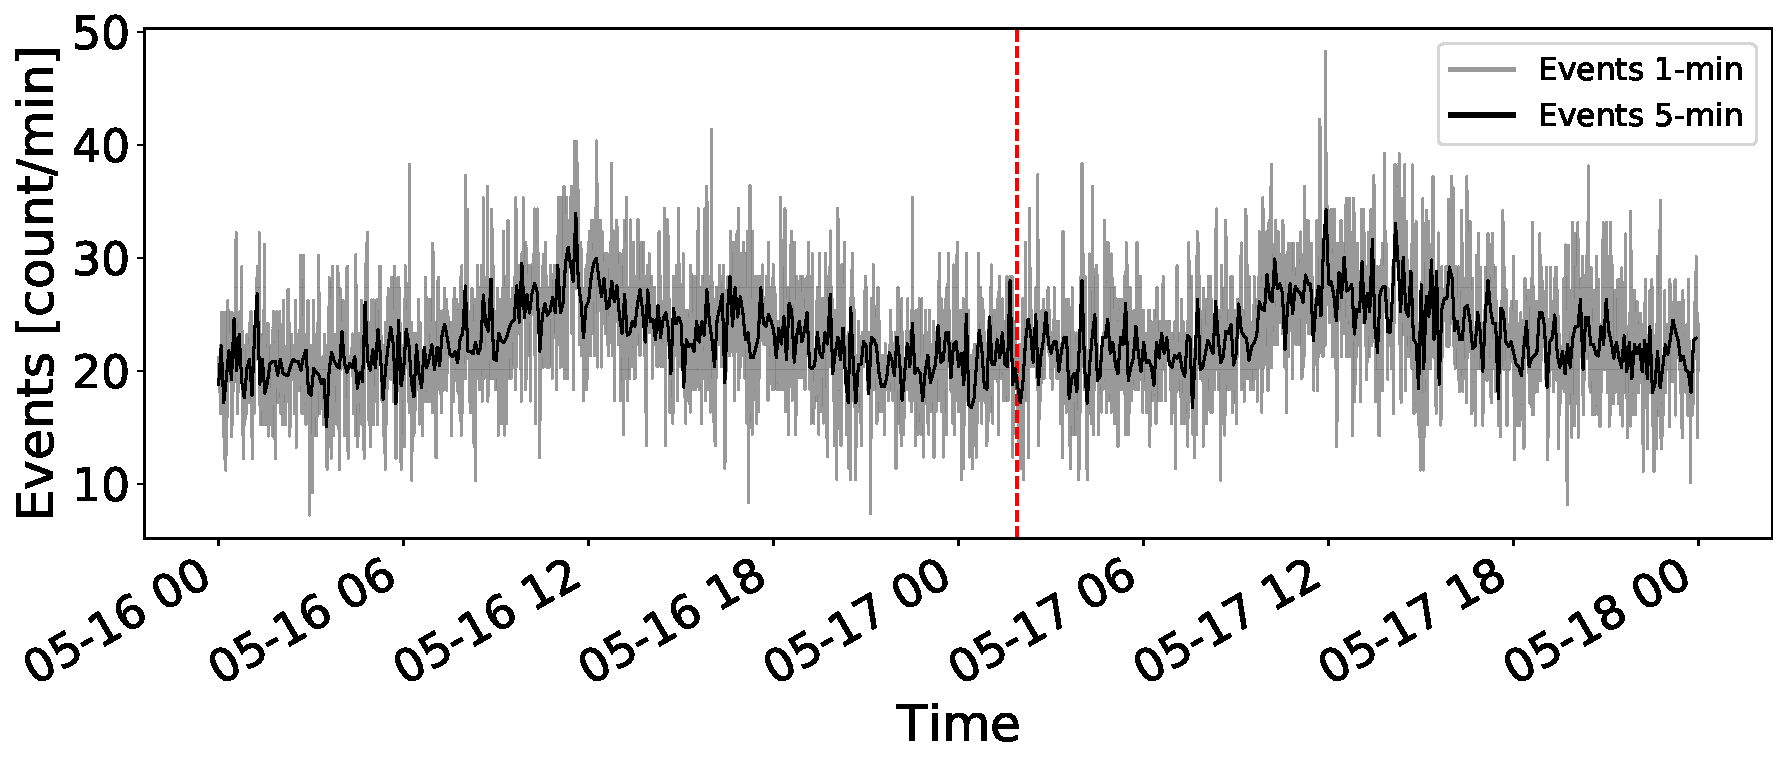
\includegraphics[width=0.48\columnwidth]{GLE71_8001_Pcorr.pdf}
		\label{fig:GLE71_8001_Pcorr}} \\
	
	
	\caption{Pressure corrected HiSPARC data for 2 stations around the epoch of GLE 71. The top panel of each subplot shows the minute-averaged trigger events between detectors within the station, while the bottom panel shows the mean-shifted, minute-averaged counts by each individual detector in the station. The vertical red, dashed line depicts the approximate onset time of the GLE.}
	\label{fig:GLE_71_Pcorr}
\end{figure}


\begin{figure}[ht]
	\centering
	\subfloat[HS 501 (Nikhef)]{
		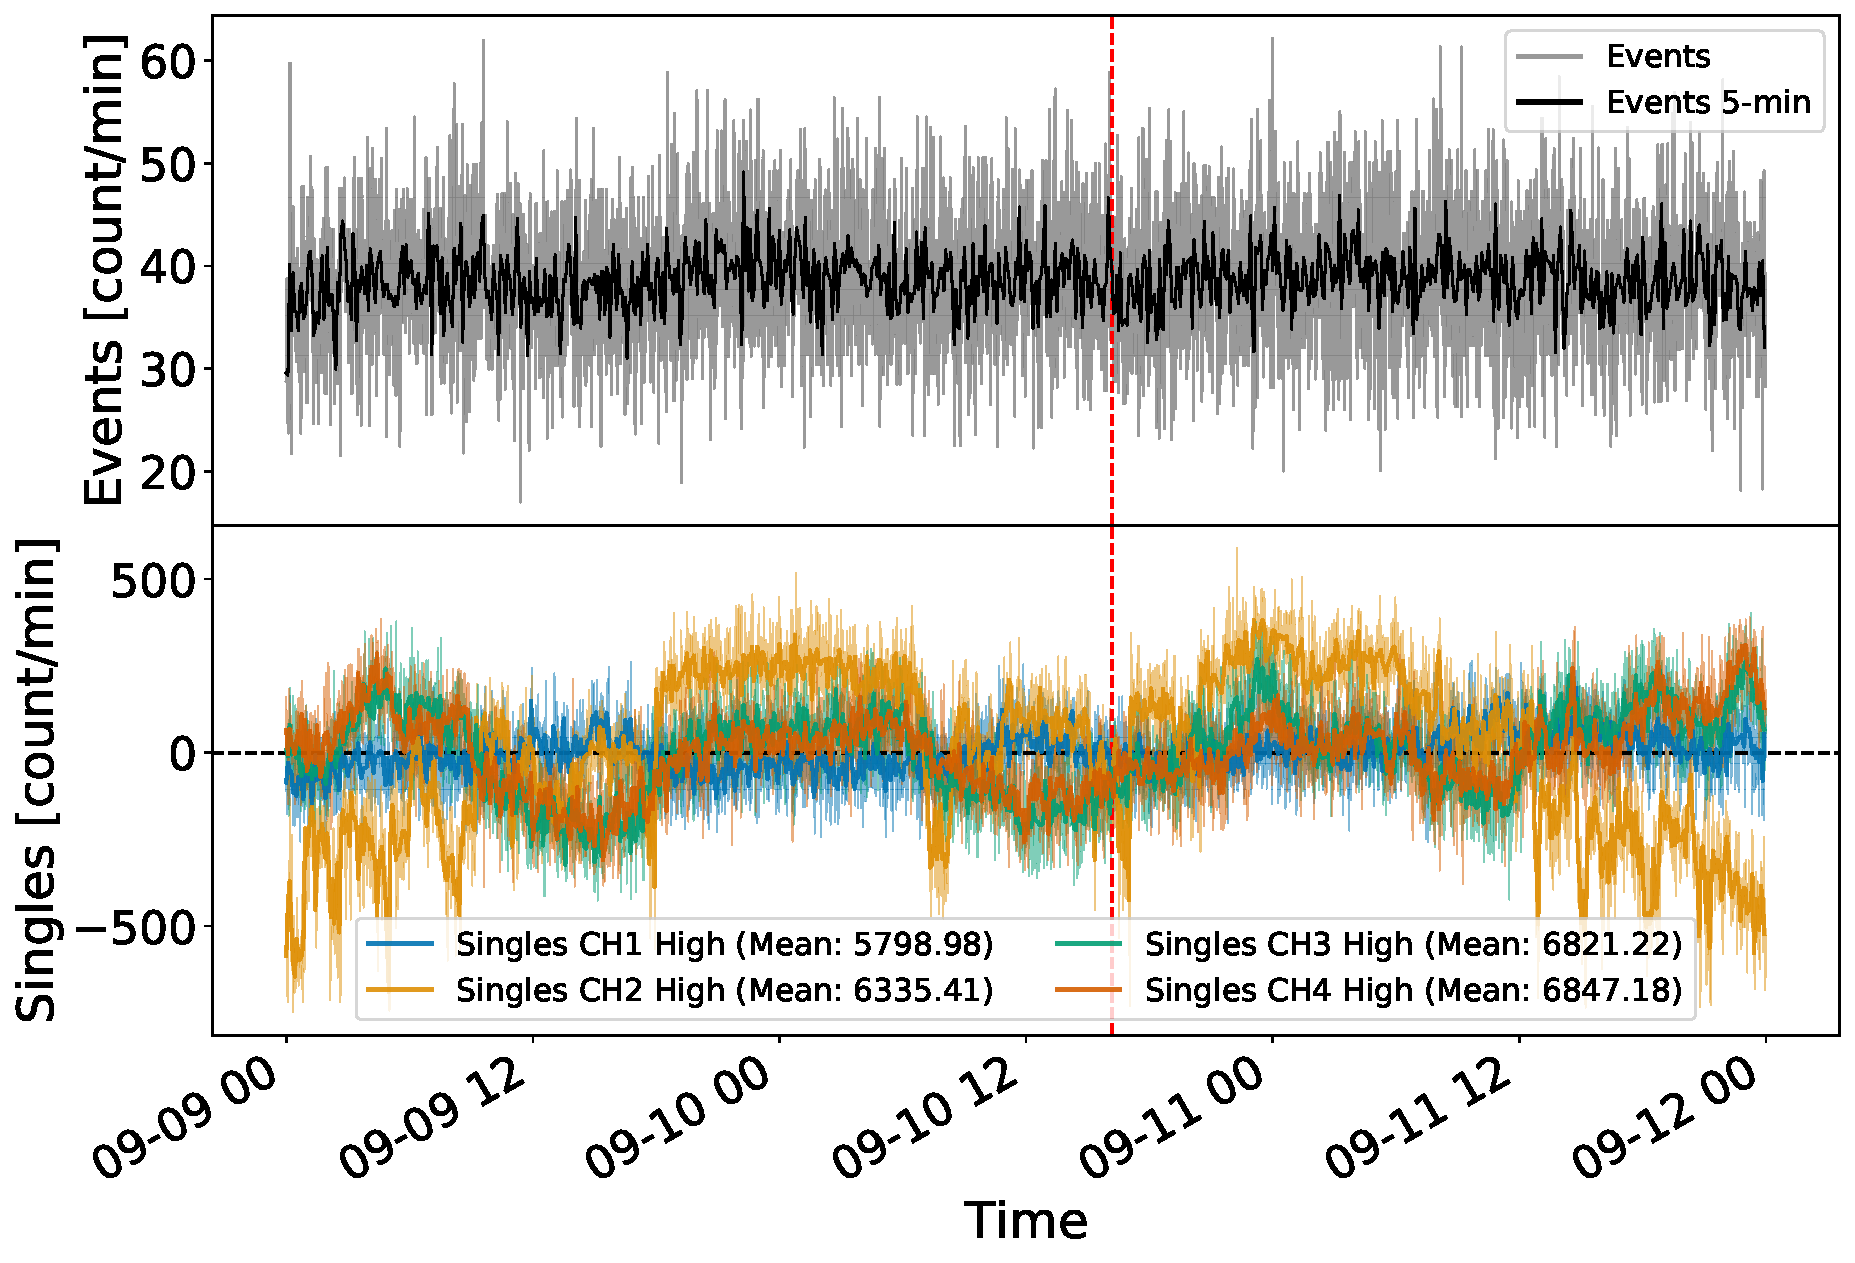
\includegraphics[width=0.48\columnwidth]{GLE72_501_Pcorr.pdf}
		\label{fig:GLE72_501_Pcorr}}
	%\qquad
	\subfloat[HS 203 (College Hageveld)]{
		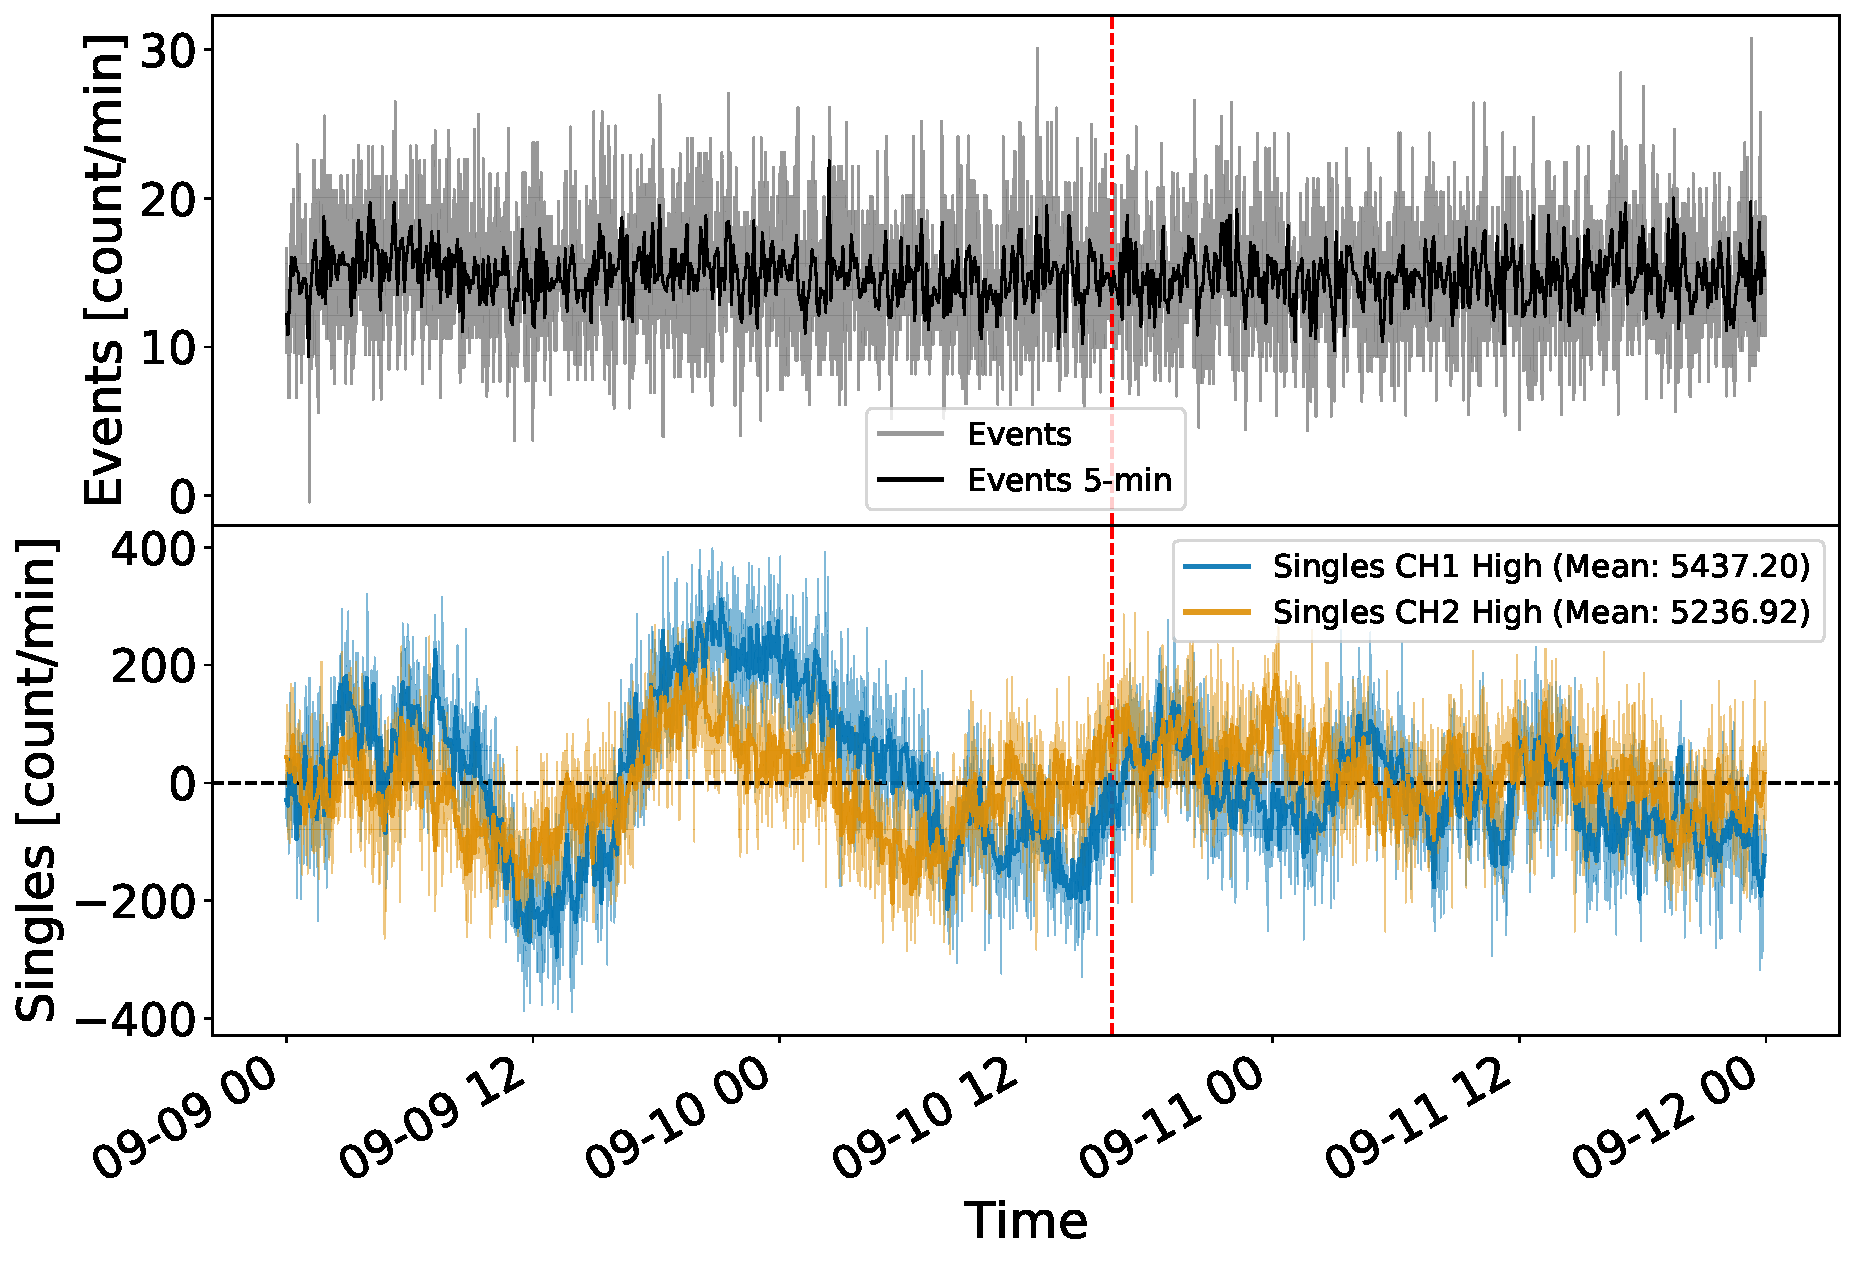
\includegraphics[width=0.48\columnwidth]{GLE72_203_Pcorr.pdf}
		\label{fig:GLE72_203_Pcorr}} \\
	
	
	\caption{Pressure corrected HiSPARC data for 2 stations around the epoch of GLE 72. The top panel of each subplot shows the minute-averaged trigger events between detectors within the station, while the bottom panel shows the mean-shifted, minute-averaged counts by each individual detector in the station. The vertical red, dashed line depicts the approximate onset time of the GLE.}
	\label{fig:GLE_72_Pcorr}
\end{figure}

There are no clear \glspl{gle} observations in the pressure corrected HiSPARC data. We believe this is due to the a mixture of the reasons discussed above: a high rigidity cut-off of the HiSPARC stations as \glspl{gle} are caused by \glspl{sep} with a lower energy, and too few additional muons produced during these most recent \glspl{gle}.


%%%%%%%%%%%%%%%%%%%%%%%%%%%%%%%%%%%%%%%%%%%%%%%%%%%%%%%%%%%%%%%%%%%%%
\subsection{Pressure Corrected Observations of Forbush Decreases}

The search for evidence of \glspl{fd} was re-conducted, this time within the pressure corrected HiSPARC data. Figure~\ref{fig:FD_201207_8001_Pcorr} and Figure~\ref{fig:FD_201412_501_Pcorr} shows the pressure-corrected HiSPARC observations around the epochs of a \gls{fd} in July 2012 and December 2014, respectively.

\begin{figure}[ht]
	\centering
	\includegraphics[width=0.65\columnwidth]{FD_201207_8001_Pcorr.pdf}
	\caption{HS 8001 (Eindhoven)}
	\label{fig:FD_201207_8001_Pcorr}
\end{figure}



\begin{figure}[ht]
	\centering
	\includegraphics[width=0.65\columnwidth]{FD_201412_501_Pcorr.pdf}
	\caption{HS 501 (Nikhef)}
	\label{fig:FD_201412_501_Pcorr}
\end{figure}


There are no clear \glspl{fd} observations in the pressure corrected HiSPARC data shown in Figure~\ref{fig:FD_201207_8001_Pcorr} and Figure~\ref{fig:FD_201412_501_Pcorr}...

[... introduce the last pressure corrected data plots...]

\begin{figure}[ht]
	\centering
	\subfloat[HS 501 (Nikhef)]{
		\includegraphics[width=0.48\columnwidth]{FD_GLE72_501_Pcorr.pdf}
		\label{fig:FD_GLE72_501_Pcorr}}
	%\qquad
	\subfloat[HS 203 (College Hageveld)]{
		\includegraphics[width=0.48\columnwidth]{FD_GLE72_203_Pcorr.pdf}
		\label{fig:FD_GLE72_203_Pcorr}} \\
	
	
	\caption{Pressure corrected HiSPARC data for 2 stations in an epoch where there were two FDs close to the onset of GLE 72. The top panel of each subplot shows the minute-averaged events data, while the bottom panels show the mean-shifted, minute-averaged counts by each individual detector in the stations. The vertical blue-dashed lines show the approximate onset-times of the FDs and the red-dashed line depicts the approximate onset-time of the GLE.}
	\label{fig:FD_GLE72_Pcorr}
\end{figure}

[...insert comments on the lack of clear fds here...]



%%%%%%%%%%%%%%%%%%%%%%%%%%%%%%%%%%%%%%%%%%%%%%%%%%%%%%%%%%%%%%%%%%%%%
%%%%%%%%%%%%%%%%%%%%%%%%%%%%%%%%%%%%%%%%%%%%%%%%%%%%%%%%%%%%%%%%%%%%%
\section{Discussion}\label{sec:HS_discussion}

Throughout this chapter the feasibility of using the HiSPARC network of muon detectors has been analysed. This has involved performing cosmic ray air shower simulations using \gls{corsika} and performing backwards


%%%%%%%%%%%%%%%%%%%%%%%%%%%%%%%%%%%%%%%%%%%%%%%%%%%%%%%%%%%%%%%%%%%%%
%%%%%%%%%%%%%%%%%%%%%%%%%%%%%%%%%%%%%%%%%%%%%%%%%%%%%%%%%%%%%%%%%%%%%
\section{Conclusion}\label{sec:HS_conclusion}

...

... Need to add in that we should suggest to place a HiSPARC detector at a higher latitude (and altitude) to reduce the rigidity cut-off, and increase the muon count rate and lower the pcr energy sensitivity...

We leave the reader with the following points:

\begin{enumerate}
	\item{...}
	\item{...}
	\item{...}
\end{enumerate}